\documentclass[twoside,phd, openright,titlepage]{iitkgp}

\newcommand{\dotrule}[1]{%
\parbox[t]{#1}{\dotfill}}

\newtheorem{problem}{Problem}[chapter]

\newcommand{\remove}[1]{}
\newcommand{\argmax}{\mathop{\mathrm{argmax}}}
\newcommand{\complain}[1]{\textcolor{red}{#1}}

    \newtheorem{theorem}{Theorem}[section]
    \newtheorem{lemma}[theorem]{Lemma}
    \newtheorem{proposition}[theorem]{Proposition}
    \newtheorem{corollary}[theorem]{Corollary}
    \newtheorem{definition}[theorem]{Definition}
    \newtheorem{observation}[theorem]{Observation}

    \newenvironment{proof}[1][Proof]{\begin{trivlist}
    \item[\hskip \labelsep {\bfseries #1}]}{\end{trivlist}}
    %\newenvironment{definition}[1][Definition]{\begin{trivlist}
    %\item[\hskip \labelsep {\bfseries #1}]}{\end{trivlist}}
    \newenvironment{example}[1][Example]{\begin{trivlist}
    \item[\hskip \labelsep {\bfseries #1}]}{\end{trivlist}}
    \newenvironment{remark}[1][Remark]{\begin{trivlist}
    \item[\hskip \labelsep {\bfseries #1}]}{\end{trivlist}}

    \newcommand{\qed}{\nobreak \ifvmode \relax \else
          \ifdim\lastskip<1.5em \hskip-\lastskip
          \hskip1.5em plus0em minus0.5em \fi \nobreak
          \vrule height0.75em width0.5em depth0.25em\fi}


\newcommand{\tuple}[1]{\langle #1\rangle}


%\usepackage{subfigure}
\usepackage{latexsym}
%\usepackage{graphics}
\usepackage{psfig}
%\usepackage{graphicx}
\usepackage{amsmath}
\usepackage{amsfonts}
\usepackage{amssymb}
\usepackage{xpatch}
\usepackage[toc]{appendix}
% \usepackage{eufrak}
%\usepackage{setspace}
\usepackage[english]{babel}
%%%%%%%%%%%%%%%%%%%%%%%%%%%%%%%%%%%%%%%%%%%%%%%%%%%%%%%%%%%%%%%%%%%%%%%%%%%%%%%%%%%%%%%%%%%%%%%%%%%%


\usepackage{verbatim}
\usepackage{multirow}
\usepackage{colortbl}
\definecolor{lgray}{gray}{0.8}

 \usepackage{ifpdf}
 \ifpdf
 \usepackage[pdftex]{graphicx}
 \else
 \usepackage{graphicx}
 \fi

\usepackage{epsfig}
% \usepackage{graphicx}
%%\usepackage{acronym}
\usepackage{fancyhdr}
  \fancyhead{}
  %\fancyhead[LO]{\slshape \rightmark}
  \fancyhead[RO]{\textbf{\rightmark}}

%  \fancyhead[RE]{\slshape \leftmark}
  \fancyhead[LE]{\textbf{\leftmark}}
  \fancyfoot{}
  \fancyfoot[CO,CE]{\textbf{\thepage}}
  \pagestyle{fancy}
  \renewcommand{\chaptermark}[1]{\markboth{\chaptername \ \thechapter \ \ #1}{}}
  \renewcommand{\sectionmark}[1]{\markright{\thesection \ \ #1}}

\newcommand{\captionfonts}{\small}
\usepackage{cite}
%\usepackage[lined,algonl,algochapter,algoruled]{algorithm2e}
\usepackage[linesnumbered,ruled,vlined]{algorithm2e}
% \usepackage{algorithm}
\usepackage{algorithmic}
\usepackage{makeidx}
\makeindex
%\usepackage{amsmath,amssymb}
\usepackage[hyphens]{url}
\urlstyle{rm}
% \usepackage{subfigure}

%\usepackage[cmex10]{amsmath}
\usepackage{ulem} \normalem
\usepackage{amsmath, amssymb}%amsthm, amssymb}
\usepackage[figuresright]{rotating}
\usepackage{tikz}
\usepackage{tikz-dependency}
\usepackage[bookmarks=true,plainpages=false,pdfpagelabels]{hyperref}
\hypersetup{linktocpage}

%\usepackage[colorlinks=true,linkcolor=black,urlcolor=blue]{hyperref}
% \usepackage{dropping}
\usepackage{paralist}
\usepackage{sectsty}
\chapterfont{\LARGE}
\chaptertitlefont{\Huge}
\sectionfont{\Large}
\usepackage{pslatex}
\usepackage{subfig}
\usepackage{float}
% following is for making list of abbreviations
\usepackage{nomencl}
% \makenomenclature
\usepackage{titlesec}
\usepackage{enumitem}
\newcommand{\specialcell}[2][l]{%
  \begin{tabular}[#1]{@{}l@{}}#2\end{tabular}}


%========================================================================
% configure
%========================================================================
\Year{2020}
\Month{May}
\Author{Abhijit Mondal}
\degree{Doctor of Philosophy}

\TitleTop{To Be Decided}
\TitleBottom{}

% Your research advisor
\AdvisorA{Sandip Chakraborty}

\AuthorDeclaration{
	\noindent I certify that 
	\begin{itemize}
		\item[a.]  The work contained in this thesis is original and has been done by myself under the general supervision of my supervisor.
		\item[b.]  The work has not been submitted to any other Institute for any degree or diploma.
		\item[c.]  I have followed the guidelines provided by the Institute in writing the thesis.
		\item[d.]  I have conformed to the norms and guidelines given in the Ethical Code of Conduct of the Institute.
		\item[e.]  Whenever I have used materials (data, theoretical analysis, and text) from other sources, 
		I have given due credit to them by citing them in the text of the thesis and giving their details in 
		the references. 
		\item[f.]  Whenever I have quoted written materials from other sources, I have put them under quotation marks and 
		given due credit to the sources by citing them and giving required details in the references.
	\end{itemize}
}

\DedicatedTo{\bf Dedicated to my parents}

\ApprovalSignatures{
	\begin{table}[ht]
		\begin{tabular}{p{5.4cm}p{4cm}p{5cm}}
			
			&&\\
			&&\\
			\noindent\line(100,0){100} 	 & \line(100,0){100}			& \line(100,0){100}\\
			(Member of DSC) 			 & (Member of DSC)				& (Member of DSC)\\
			Dr. Animesh Mukherjee		 & Dr. Bivas Mitra    			& Dr. Goutam Das \\
			Professor   				 & Professor					& Professor\\
			Department of CSE            & Department of CSE 			& G.S.S School of Telecommunication.  \\
			IIT Kharagpur, India  		 & IIT Kharagpur, India         & IIT Kharagpur, India\\          
			
			
			&&\\
			&&\\
			
			\noindent\line(100,0){100} 			&& \line(100,0){100}\\
			(Supervisor) 				        && (Chairman) \\
			Dr. Sandip Chakraborty				&& Dr. Niloy Ganguly  \\
			Professor 				        	&& Professor \\
			Department of CSE 		            && Department of CSE \\
			IIT Kharagpur, India				&& IIT Kharagpur, India \\    
			
			
			&&\\
			&&\\
			
			
			\noindent\line(100,0){100} 			&& \line(100,0){100}\\
			(Head of the Department) 			&& (External Examiner) \\
			Dr. Dipanwita Roy Chowdhury			&& \\
			Professor							&& \\
			Department of CSE					&& \\
			IIT Kharagpur, India				&& \\    
		\end{tabular}
	\end{table}
}


%================================================================
% ------------------------- Fill in these fields for the preliminary pages ----------------------------
%
 \begin{document}
% \font\Hin=''gargi:script=hin''
\thispagestyle{empty}
\begin{center}

\vspace{4.0in}

\Large{\bf \vspace{0.06in} \TitleFull}

\vspace{7.3in}


\noindent\rule[-1ex]{\textwidth}{1pt}\\[-1.8ex]
\noindent\rule[-1ex]{\textwidth}{5pt}\\[1.5ex]

\end{center}

\begin{flushright}
\large{\textbf{\studname}}
\end{flushright}

\clearemptydoublepage



%%%%%%%%%%%%%%%%%%%%%%%%%%%%%%%%%%%%%%%%%%%
\Acknowledgments{

\addcontentsline{toc}{chapter}{Acknowledgements}
\fontsize{12}{13}\selectfont %\dropping[0cm]{2}
Many people supported me during the journey, and it is my honor to acknowledge them. At first, I like to express my gratitude towards my supervisor Prof. Sandip Chakraborty for his immense help, motivation, guidance to carry out this work. His continuous support in the form of discussions, constructive criticisms, and clear understandings has helped me proceed in the right direction. I am really indebted to him for giving me a wide exposure to the field of computer networks and online video streaming and helping me to contribute constructively to this field. In this entire tenure, he was not only my supervisor but also a friend whom I could always count. It was impossible to complete this work without his support.

I will forever be thankful to Dr. Niloy Ganguly for encouraging me to take up this Ph.D. journey and the support he provided both on the research and career front. I would extend Prof. Animesh Mukherjee, Prof. Bivas Mitra, and Prof. Gautam Das to serve on my doctoral scrutiny committee and for their valuable advice and suggestions. I am privileged to thank Prof. Arobinda Gupta, Prof. Payan Goyel, Prof. Palash Dey for the lessons and experience during several classes and TA sessions. It is an honor to get in touch with Rajeev Shorey, and I thank him for introducing me to the extensive network of researchers. I would like to thank Bappa da, Hoimanti di, Ashokbabu, Swapanbabu, Prasunda, and all other office members for being helpful in sorting out all the official work.

It is my pleasure to thank Ayan da, Subhrangsu da, Soumadip, Snigdha, Soumyajit, Bishakh, Basabdatta di (BD) for the company and support throughout the period and the encouragement to finish the thesis. I am also grateful to Surjya da, Ayan, Bidisha, Satadal, Rohit, Madhumita, Soumajit (halum), Abir da for the inspiration they provided. The campus life would not be memorable without Bijoy, Anupam, Sueet, Alapan, Ashutosh, Suravi. I thank every member of CNeRG for being there whenever I needed some help. My acknowledgment would not complete without saying thanks to Pala for the various insight before and during the period.

My greatest strength comes from my family. My parents and my sister have been my greatest source of inspiration. Without their patience, constant encouragement, support, unparalleled love, prayers, and well wishes, I could never have completed this endeavor. I am what I am because of them. My sister, Dipa, was always there for me and always ready to bring a smile to me.

% {\chancery 
%This thesis would not have seen the light of day without the help and support of many people. I would like to express my gratitude towards my supervisor Prof. Sudeshna Sarkar for her immense help, motivation, and guidance to carry out this work. Her continued support in the form of discussion, constructive criticism, and clear understanding has helped me to proceed in the right direction. I am really indebted to her for giving me a wide exposure to the field of natural language processing and helping me to contribute constructively to this field. Without her invaluable advice and supervision, it would not be possible to complete this work. I am grateful to Prof. Pabitra Mitra, Prof. Jayanta Mukhopadhyay, Prof. Pawan Goyal, and Prof. Shamik Sural for serving on my doctoral scrutiny committee and for their valuable advise and suggestions. Finally, I would like to thank Prof. Sudebkumar Prasant Pal, Prof. Debdeep Mukhopadhyay, Prof. Dipanwita Roy Chowdhury, Prof. Pallab Dasgupta and Prof. Niloy Ganguly for teaching me different subjects that helped me in carrying out my research. I would like to thank Bappada, Ashokda, Swapanbabu, Shibuda, Prasunda, Prasenjitda, Durgada and all other office members for being helpful in sorting out all the official work.
%
%% CHANGE THIS PARA
%I feel blessed to have friends like Rajorshee (Jalu), Subhrangshu (\textit{SM}), Abhijit, Ashutosh, Soumadip, Bijoy, A(-CM)bhik, Rajibda and Arnab. Without their company and support, it would have been difficult to complete my PhD. I would like to acknowledge my gratitude towards my seniors Joyda, Kunalda, Aritrada, Sumantada, Sudakshinadi, Antaradi, Priyankadi and Subhasishda for their unconditional support and valuable advice. I thank Tapas, Bidisha, Kalyani, Anirban, Paheli, Parthada, Devleena, Alapan, Arpita, Anupam, Subhajit, Debasish, Sibendu, Pawan, Aliba, Avik and Anupamda for making my stay at IIT Kharagpur a memorable one.
%
%I would like to take this opportunity to thank Dr. Mandar Mitra and Mr. Niharendu Mukhopadhyay who have always inspired me with their unconditional support and encouragement throughout this journey.
%
%My greatest strength comes from my family. My parents have been my greatest source of inspiration. Without their patience, constant encouragement, support, unparalleled love, prayers and well wishes, I could never have completed this endeavour. I am what I am because of them. I would also like to express my gratitude towards my aunts, brothers and sisters-in-law for their constant support and encouragement. I am grateful towards my niece and nephew for being  constant sources of smile for me.\\\\
\begin{flushright}
\medskip

\studname\\

\end{flushright}

}

%%%%%%%%%%%%%%%%%%%%%%%%%%%%%%%%%%%%%%%%%%%%%%%%%%%%%%%%%%%%%%%%%%%%%%%%%%%%%%%%%%%%%%%%%%%%%%%%%%%%%%%%



\Abstract{
\addcontentsline{toc}{chapter}{Abstract}
\fontsize{12}{13}\selectfont %\dropping[0cm]{2}
\begin{comment}
In the era of low-cost, high-end smartphones, smart TVs, and cheap 4G-LTE data plans, video streaming becomes an essential service on the Internet. Most online video streaming services are adaptive video streaming, and adaptive bitrate algorithms play an important role in maintaining Quality of Experience, data usages, and energy consumption. From the inception in 2009, several researchers proposed different ABR algorithms and changes in the architecture to improve the QoE, energy efficiency. However, there is much to improve in the video streaming system to support more advanced devices, scale to millions, and reduce energy requirements. In this work, we have tried to analyze the existing services and suggested a few improvements.

Video streaming services contribute most of the Internet traffic globally and make every player on the Internet to adapt and improve their technologies to support the growing users. It is so massive that during the COVID'19 pandemic, streaming providers decided to drop their top-quality to relieve Internet service to get paced to support the sudden growth in work-from-home users. It also raises a question to the research community why ABR algorithms are not enough to handle excess bandwidth requirements. Though we do not know the question, it provides perspective regarding this domain's importance and motivates many to dig deep. This type of issue motivates us to understand how the existing system works what can be done to improve it.

YouTube is a major video streaming provider and the pioneer of web-based video streaming service. As per their press release, it serves a billion videos to 30 million users every day. It is interesting the see how YouTube serve adaptive video to users. As the literature lacks the YouTube adaptive streaming system's details, we perform experiments to reveal it. We used our homegrown tools to get request-response pair during video playback in a browser for ~500 YouTube videos and analyzed it. Our analysis finds that YouTube uses an opportunistic upscale and conservative downscale of video quality based on network quality and adapts segment length before changing quality. We also observed that YouTube sometimes tries to download the same segment of different quality, which can cause data wastage. However, our calculation reveals that data wastage is negligible.

By 2017, Google made Quick Internet UDP Connect or QUIC as the default transport protocol for all its services from the Chrome browser. We experiment to find out its impact on the video streaming services, especially on the ABR algorithms. The experiment has two parts. First, we analyzed YouTube and found that the QUIC provides better video quality with lower rebuffering than TCP. In the second part, we compare popular ABR algorithms' performance over QUIC and TCP and found that these ABR algorithms are not well suited for QUIC. When we dig deep, we realized that problem lies in the userspace implementation of QUIC. In this work, we also wanted to know the impact of video streaming during mobility on energy efficiency. We studied power consumption in various commodity smartphones while playing YouTube videos with different mobility states in different cities. In this study, we observed that YouTube does not care about the instantaneous throughput or the radio state, which can cause a severe impact on power consumption.

With last observations, we design the EnDASH ABR algorithm that reduces power consumption during the video streaming by carefully scheduling the segment downloading based on the various device-related parameters, including cellular radio, battery, and device movement. EnDASH divides the entire playback session into slots. At the beginning of each slot, it first estimates the estimate the average throughput and then selects the maximum playback buffer length based on the slot based on the observations last slot. The buffer change in playback buffer length triggers the rescheduling in segment downloading. The EnDASH also has a module that decides the video quality for each segment, which further reduces power consumption. It requires three different learning engines, a) Throughput estimation engine, b) Buffer length prediction engine, and c) quality selection engine. The throughput estimation engine is based on random forest reinforcement learning. The buffer length prediction engine and quality selection engine are designed based on an actor-critic based recurrence neural network. We find that EnDASH provides better energy efficiency during evaluation than the existing ABR algorithm with a slight compromise in the QoE.

After saving energy, we decided to save some data usages. So, we developed FLiDASH, a federated adaptive live streaming system that exploits players' locality by forming coalitions. We observed that mega-event live streamers are localized, and most of the cases are connected via a local network. However, the current setup does not exploit the local network. Instead, every player downloads the segment on their own. FLiDASH utilizes the local network to find out players that can be communicated without involving the Internet. Then it forms a coalition among players that have similar quality targets. Every player in a coalition contributes to QoE's improvement by downloading based quality video it can download. We use the moving leader concept, where the leader is responsible for downloading a segment and deciding the leader for the next segment. These two algorithms work in a way so that a player with the lowest download speed gets to download the furthest segment in the long run. Our evaluation reveals that FLiDASH can improve the QoE for a coalition while reducing the server load and the network load. We also find that every player gains QoE and average quality by using FLiDASH than using any other ABR algorithms.

In the thesis, we analyze YouTube's adaptive streaming behavior and find interesting insights. We also analyzed the energy efficiency of YouTube and ABR's compatibility with different ABR algorithms. With study, we develop EnDASH to save energy in smartphones during video playback. Later we save data usages and server load by sharing segments among video players. In the future, we have to find an ABR algorithm for better compatibility with QUIC and TCP. It is also important to find a way to deploy a machine learning-based ABR algorithm, which is difficult now due to resource and technology requirements.

\end{comment}

\textbf{Keywords:}
}

%%%%%%%%%%%%%%%%%%%%%%%%%%%%%%%%%%%%%%%%%%%%%%%%%


\fussy %\makenomenclature
%\begin{document}

 % Start page counting in roman numerals
 \frontmatter

 \makepreliminarypages
 %\singlespace

%\listoffigures
 \clearemptydoublepage

% \listoftables
 \clearemptydoublepage
%\listofacronyms[acrodefs][u]

%\listofsymbols
%\clearemptydoublepage
%\thispagestyle{empty}
% to print list of nomenclature :
% open command prompt in winedt and write: makeindex thesis.nlo -s nomencl.ist -o thesis.nls
\fontsize{12}{13.2}\selectfont
%

%\printnomenclature[1in]
%\thispagestyle{empty}

%\thispagestyle{empty}
%
 \fancyhead[RO]{\textbf{\rightmark}}

%  \fancyhead[RE]{\slshape \leftmark}
  \fancyhead[LE]{\textbf{\leftmark}}
  \fancyfoot{}
  \fancyfoot[CO,CE]{\textbf{\thepage}}
  \pagestyle{fancy}
  \renewcommand{\chaptermark}[1]{\markboth{\chaptername \ \thechapter \ \ #1}{}}
  \renewcommand{\sectionmark}[1]{\markright{\thesection \ \ #1}}

%%%%%%%%%%%%%%%%%%%%%%%%%%%%%% Abstract %%%%%%%%%%%%%%%%%%
% \clearemptydoublepage
% \addcontentsline{toc}{chapter}{Abstract}
% \include{HeadTail/abstract}
% \thispagestyle{empty}

%%%%%%%%%%%%%%%%%%%%%%%%%%%%%%%%%%%%%%%%%%%%%%%%%%%%%%%%%

\fontsize{12}{13.5}\selectfont

\tableofcontents


%%%%%%%%%%%%%%%%%%%%%%%%%%%%%% Abbreviation %%%%%%%%%%%%%%%%%%
% \fontsize{12}{14.5}
% 
% \clearemptydoublepage
% 
% \addcontentsline{toc}{chapter}{Symbols and Abbreviations}
% \include{abbr}
% \thispagestyle{empty}

%%%%%%%%%%%%%%%%%%%%%%%%%%%%%%%%%%%%%%%%%%%%%%%%%%%%%%%%%%%%%%%
\clearemptydoublepage
    \listoffigures  
\thispagestyle{empty}
\clearemptydoublepage



% \addcontentsline{toc}{chapter}{List Of Algorithms}
%  \chapter*{List of Algorithms} 
\fontsize{12}{14.5}\selectfont
\noindent
\def\arraystretch{1.6}
 \begin{tabular}{llr}
 3.1 & Algorithm for Finding Maximal Chunks \dotrule{0.41\textwidth}   &   43\\ 
 7.2 & Distributed Offline Algorithm for the Dist-MaxProfitMaxEVCharging Pro-    &     \\
     & blem                                                                 \dotrule{0.79\textwidth}   &   164\\
 \end{tabular}
\def\arraystretch{1} 

% \clearemptydoublepage

\fontsize{12}{14.5}\selectfont
 \mainmatter

\abovedisplayskip=5pt \belowdisplayskip=5pt
\renewcommand{\baselinestretch}{1.37}\small\normalsize
\parskip 7pt
%
\makeatletter
\newlength{\mySpaceUnder}
\newlength{\mySpaceOver}
\setlength{\mySpaceUnder}{.15cm plus .2ex}  % 4cm as an example ;-)
\setlength{\mySpaceOver}{.4cm plus -1ex minus-.2ex}   % 3cm as an example
\renewcommand\section{\@startsection {section}{1}{\z@}%
                                   {\mySpaceOver}%
                                   {\mySpaceUnder}%
                                   {\normalfont\Large\bfseries}}
%
\newlength{\mySpaceUndera}
\newlength{\mySpaceOvera}
\setlength{\mySpaceUndera}{.1cm plus .1ex}  % 4cm as an example ;-)
\setlength{\mySpaceOvera}{.3cm plus -1ex minus-.1ex}   % 3cm as an example
\renewcommand\subsection{%
 \def\@seccntformat##1{\csname the##1\endcsname\hspace{.25in}}
 \@startsection{subsection}{1}{\z@}{\mySpaceOvera}%
                                   {\mySpaceUndera}%
                                   {\normalfont\large\bfseries}
}
%
%
\renewcommand\subsubsection{%
 \def\@seccntformat##1{\csname the##1\endcsname\hspace{.25in}}
 \@startsection{subsubsection}{1}{\z@}{.2cm}%
                                   {.01cm}%
                                   {\normalfont\em\bfseries}
}
%
\makeatother
%
\newenvironment{my_item}{
\begin{enumerate}
  \setlength{\itemsep}{2pt}
  \setlength{\parskip}{0pt}
  \setlength{\parsep}{0pt}
}{\end{enumerate}}
%
%
\fontsize{12}{14.5}\selectfont

\chapter[Introduction]
{Introduction}
\label{chapter:intro}
\noindent

\graphicspath{{Chapters/02.Background/}}

%\section{Introduction}
Online video streaming is the most popular service on the Internet. The pervasive penetration of smartphone and availability of cheap LTE network make it even easier for reach to millions of users.
%The introduction of the video streaming system over the HTTP and in build player in HTML5 makes it easier to start a new video streaming service on the one hand. On the other hand, the LTE network's pervasive penetration makes it easier for smartphone users to watch online videos. On top of HTTP and HTML5, dynamic adaptation of the audio-video quality allows stream providers to make the service tolerant to frequent network change. These technologies gain the attention of researchers all around the globe. In this work, we discuss the technological advancement for video streaming using HTTP.
Video streaming can be primarily categorized into three categories: i) static video or video-on-demand (VoD) streaming, ii) live video streaming, and iii) interactive video streaming. Video streaming services like YouTube, NetFlix, Prime videos fall into the video-on-demand category. Here the videos are prerecorded and preprocessed. YouTube-Live, Periscope, Twitch provide live video streaming Category. The only difference between VoD and live video streaming is that videos are not preprocessed in live streaming as it is not ready yet. The services like video conferencing, webinars are fall in the third category, the interactive video. The interactive online videos are not only bidirectional but also extremely delay-sensitive. Unlike VoD or live streaming, it is okay for interactive video streaming to drop several frames than stall for data. So, the technology required for the interactive video is very different in every aspect. In our work, we concentrated on the VoD and live video streaming over HTTP only.

HTTP is a widely accepted protocol as it serves the World-Wide-Web (WWW). Most of the firewalls, proxies, and NAT-boxes allow HTTP protocol. HTTPS, the secure version of HTTP, is equally acceptable for the network administrator of different organizations. So, the HTTP(S) based video streaming services also allowed by those firewalls, proxies, and NAT boxes. This one feature favored HTTP(S) based video streaming over the existing video streaming system.

On top of the HTTP-based video streaming system, service providers can now adapt video quality according to the available network quality. It reduces the rebuffering significantly. Currently, most online video services support adaptive video streaming as it provides a better quality of experience to the viewers. Several technologies like MPEG-DASH (dynamic adaptive streaming over HTTP), Apple's HLS, and SmoothStream by Microsoft developed to provide dynamic adaptive streaming. Although different organizations develop these technologies, they work almost identically. In our work, we concentrate on the DASH only as it is a guideline than a product and the open-source implementation of DASH is available.

DASH or DASH-like video streaming systems changes video quality on the fly running a special algorithm call adaptive bitrate algorithm (ABR). The selection of ABR is crucial as the overall quality of experience is dependent on this algorithm. It is the ABR algorithms' job to provide minimal rebuffering while maintaining better video quality. In our survey, we first discuss the details of the DASH and different components of DASH. We then discuss DASH's application on YouTube, a major video streaming provider, and the latest research on the ABR to provide better QoE for both VoD and live streaming in different scenarios.

%\subsection{DASH}
%
%%
%Dynamic Adaptive Streaming over HTTP (DASH), also referred to as MPEG-DASH, is an adaptive bit-rate solution for video streaming, which enables client-operated video delivery over HTTP.
%%
%DASH is implemented by breaking down the video content into small segments, each worth a short duration of playback time.
%%
%For every segment of playback time, alternative versions at various bit-rates are available at the server.
%%
%The client typically requests for the highest quality segment possible under current network conditions, such that it is received (downloaded) in time for playback, without causing stalling or re-buffering. 
%%
%However, DASH is not a protocol -- it only specifies an architecture (Fig.~\ref{fig:dash}) to enable adaptive video streaming over HTTP.
%%
%Every video streaming service (e.g., YouTube, Netflix, etc.) is free to define its own implementation of the DASH modules.
%
%\subsection{ABR}
%Adaptive bitrate algorithm or ABR algorithm is the heart of the DASH. ABR decide when and which quality to download based on network quality and other parameter. Primary job of any ABR algorithm is improve user experience by selecting appropriate video quality for the a segment. As the online video streaming become one of the most popular service in the Internet, it become more prevalent to improve ABR algorithm to provide better QoE in different. The problem attract researcher from academic as well as the industries. Researcher start exploiting different areas of video streaming with a common goal, i.e. improving QoE for end user.
%
%\subsection{QoE}
%Quality of Experience is a important parameter in any field which involves end users. In case of the video streaming, QoE is metric to measure whether user have enjoyed the video or not. QoE is mostly a user perspective and it depends on several factor such as startup delay, quality flactuation, overall quality, rebuffering, audio/video device, video content. Although all this parameters are important, it is difficult to measure user dependent parameter and video content. Several researcher tried to to find best measurable metric to calculate QoE which can be acceptable. Mok \etal \cite{5990550} tried to calculate QoE from the network QoS. Infact they suggested that user QoS (or QoS of HTTP) is the QoE. 
%
%\blue{TODO: More about QoE}


\section{Motivation}
\subsection{ABR algorithms and interplay with computer networks}
ABR algorithms are an essential part of any adaptive video streaming system, as discussed in the last section. It is assumed that ABR algorithms are fair among themselves and the other type of traffic in most cases. However, during the COVID-19 pandemic, various video streaming services started dropping the highest quality of video from their service to preserve bandwidth available to the ISP as many people started working from home. At that time, the research community started questioning whether it was a fault of the video streaming system? Whether or not the existing ABR algorithms adjust themselves to lower bitrate when the load is high, or there is something wrong with the deployment of those streaming services. While we do not really know the answer, it is clear that the ABR algorithms are very important. The video streaming system needs to adapt to various network conditions. Questions like this motivate us to research the video streaming system.

Google's YouTube is one of the pioneers of video streaming over HTTP(S) and a major online video streaming player. It serves a billion videos to 30 million users daily\footnote{\url{https://blog.youtube/press/}}. To scale the service to support these huge user bases, YouTube has developed several improvements that involve content delivery networks, transport protocol and the adaptation algorithm. No doubt, YouTube gained the attention of the research community to understand the system. In the past, there were several researchers studied YouTube for better understanding. However, most of the work either explore the traffic pattern and QoE properties of YouTube\cite{gill2007youtube,krishnappa2013dashing,wamser2016modeling,wamser2015poster,6757893ieeeexp,7129790ieeeexp} or explore the trade-off between video quality and data wastage\cite{sieber2015cost,seufert2015youtube,sieber2016sacrificing}. Although these studies give an important aspect of YouTube, they failed to explore the internal parameter and streaming strategies. It is crucial to know the adaptation strategies and internal parameters of YouTube to improve the DASH-based system.

Web being Google's primary busyness, it started a project called `Make the Web Faster`\footnote{\url{https://developers.google.com/speed}}. It developed several tools and optimization to load a web page faster. Quick UDP Internet Protocol (QUIC)\cite{langley2017quic} is a product of this project where Google ditched the underlying TCP protocol and provide a new transport protocol based on the UDP. From the release of QUIC, researchers have studied the performance of it in various scenarios, including DASH based video streaming. As the QUIC work differently than TCP, and most of the ABR algorithms used in various video streaming platform are designed for TCP as the transport protocol, those ABR algorithms might not work well with QUIC. Research works like \cite{bhat2018improving,van2018empirical}, studied QUIC performance on ABR algorithm, found that buffer-based ABR algorithms are not well suited for QUIC. However, those works are performed using very old ABR algorithms, and studies are mostly simulation-based. Also, these works do not provide any insight into the root cause of the differences.

\subsection{Energy efficiency in online video streaming}
As per YouTube's report, users love to play online videos on a smartphone. It is also true for other streaming platforms. While most of the smartphone one-a-days have a huge battery capacity, it is still not enough to play videos for a long duration as video streaming is inherently energy-consuming. The uneven distribution of LTE networks, clustered crowds, and non-optimized video app can make these things even worse. Research in \cite{10.1145/2910018.2910656} shows that there is plenty of places to save energy by optimally configuring the streaming parameters like segment length, maximum buffer length, and segment download scheduling. These researches indicate that the interplay between the cellular network and the device's radio controller plays are a significant role in the energy efficiency of online adaptive video. It is important to learn various cellular network parameters and make informed adaptive decisions based on the learned parameters to make the adaptation more energy efficient.

\subsection{Live Streaming}
Live streaming is becoming an alternative to TV as the live broadcasts of most mega-events are broadcasted over the Internet using online live streaming. As more users are shifting towards online live streaming, it is becoming difficult to scale the mega-events' live streaming system. The existing literature proposes solutions by using Peer-to-Peer (P2P) networks to scale the live video streaming as players are in sync. However, P2P based live streaming suffers as most of the ISP allocate very less uplink bandwidth than downlink bandwidth to their subscriber. 
When a P2P network span over the Internet, traffic needs to go through the Internet, and this traffic will count towards the user's data connection. So, users may not take it lightly. However, in the case of mega-events, many users stay in clusters and share a common Internet backbone. One service can try to exploit the internal network to extend the service and provide better quality with lower overhead to the server and the ISP.

\section{Objective}
In this section, we discuss the objective of this thesis.

\subsection{Adaptive Bitrate Streaming over Today's Internet: A Case Study of YouTube}
The primary objective of this work is to understand the adaptive streaming mechanism of YouTube. Although the adaptation mechanism is based on DASH, we want to find the difference between DASH and YouTube, whether YouTube sends feedback to the server, whether the server takes any decision, and how it adapts the quality? We primarily focused on the triggering point of the quality switch. As YouTube is a closed source and proprietary service, the only way to understand it by reverse engineering it. To achieve the primary objective, we have to find a way to reverse engineer YouTube. Many works in the recent literature talk about the data wastage by YouTube video player. The data wastage is another parameter of interest. We want to find out the correlation between the adaptation strategies and the data wastage on YouTube.

\subsection{Transport Protocols and Mobility Choices for ABR Streaming: Performance vs. Energy Efficiency}
The performance of the ABR algorithm depends on the observed network quality. However, it highly depends on the underlying transport layer, TCP, until Google developed the QUIC. In this chapter, we like to understand if there is any difference in YouTube's streaming system behavior on both of these protocols. Similarly, we perform a similar study for DASH with DASH.JS implementation. As ABR streaming is very popular with a smartphone, a power constraint device, we want to know the energy efficiency of YouTube. 

\subsection{EnDASH - A Mobility Adapted Energy
	Efficient ABR Video Streaming for
	Cellular Networks}
Power management in a smartphone is very crucial that includes video streaming, especially when users are moving. So, we aim to develop an ABR algorithm, especially for smartphone base video streaming, to reduce battery consumption while maintaining reasonable QoE. We utilize the radio-related information available in a smartphone. Also, other information might be useful, such as GPS location, device speed, battery information. We want to find a correlation between these parameters in network condition and schedule the segment downloading in such a way so that it download most of the segments with the least energy consumption. The primary objectives can be summarized as follows:\\
a) Find the correlation between radio, battery, and other physical parameters of a device with the network quality.\\
b) Utilize these parameters to develop an ABR algorithm to reduce energy consumption while video streaming.\\
c) The ABR should provide reasonable QoE, although it might sacrifice the finest QoE to preserve energy.

\subsection{Federated Adaptive Bitrate Live
	Streaming over Locality Sensitive
	Playback Coalitions}
This work aims to reduce Internet and server load while maintaining high QoE during live streaming by exploiting the feature of synchronous playback and locality information. We want a player to find and share segments with other players in the locality during live streaming. We do not want any players to upload segments through the Internet as most users have very poor uplink and uploaded data count towards their data usage. Also, upload through the Internet means other users have to download segments from the Internet, which is equivalent if not worse than download from the CDN as per the players' perspective. It is also important that all the players contribute toward the segment downloading from CDN. It ensures fairness among players, even if they have different data plans. The primary objectives are as follows: \\
a) Exploit synchronous playback mechanism of live streaming and share segments among the player.\\
b) No data should be uploaded to the Internet during sharing.\\
c) Every player which are getting segments from other players should also share segment by downloading it directly from the CDN. \\
d) Every player should work towards improving QoE for every other player.

\section{Contribution}
This thesis consists of four contributory chapters. The significant contributions of the individual chapters are given below. 

\subsection{Adaptive Bitrate Streaming over Today's Internet: A Case Study of YouTube}
In this chapter, we perform reverse engineering over the YouTube ABR streaming algorithm to find out how it works and what are the parameters that impact the performance of ABR streaming over a large-scale Internet scenario. The contributions in this chapter are as follows. 
\begin{itemize}
	\item We illustrate a methodology to study YouTube's adaptive streaming behavior in-depth -- we identify and closely study the interplay among important parameters enabling this streaming algorithm.
	\item Our experiments reveal that YouTube adapts the {\it segment length} parameter before attempting to adjust video resolution -- a phenomenon not reported in the literature.
	\item We observe that segment length adaptation leads to much lower data wastage values on average than the ones reported by prior studies.
	\item We propose an analytical model, augmented with a machine learning-based classifier, which enables prediction of data consumption for an initial playback video quality when it is possible to estimate the network conditions a priori using existing mechanism like~\cite{Zou2015}.
\end{itemize}

\subsection{Transport Protocols and Mobility Choices for ABR Streaming: Performance vs. Energy Efficiency}
In the second contributory chapter of the thesis, we analyze various state-of-the-art ABR techniques under different transport protocols and mobility choices. This analysis gives us an idea about how ABR algorithms work in diverse scenarios, evident over today's Internet. The contributions in this chapter are summarized below. 
\begin{itemize}
	\item Like the previous chapter, we first conduct a study over YouTube to analyze YouTube ABR performance over two different transport protocols -- TCP and QUIC.
	\item We then perform a study over a controlled environment, to explore how different modern ABR algorithms like BOLA~\cite{Spiteri2016}, MPC~\cite{yin2015control}, Pensieve~\cite{mao2017neural}, etc. work over QUIC in comparison to TCP.
	\item Finally, to understand the impact of ABR streaming over the energy consumption of a mobile device, we conduct a thorough experiment using commodity smartphones and commercial cellular network connections under different mobility scenarios. We observed that arbitrary data download through ABR may impact the smartphone's energy consumption behavior when some OTT media application runs for streaming a video. 
\end{itemize}

\subsection{EnDASH - A Mobility Adapted Energy Efficient ABR Video Streaming for Cellular Networks}
This chapter develops an energy-efficient video streaming algorithm while preserving the QoE performance of the ABR mechanism. The salient contributions of this chapter are as follows. 
\begin{itemize}
	\item With the observation from previous chapters, we developed a throughput prediction engine to predict average throughput for a short future.
	\item We design an ABR algorithm based on the throughput prediction algorithms and instantaneous parameters to reduce the power consumption by optimally adjust the playback buffer lengths.
	\item We performed thorough experiments in an emulated environment to show the performance of the proposed mechanism, called \textit{EnDASH}. We observe that the proposed mechanism significantly saves energy consumption during video streaming with marginal compromise in the overall QoE. 
\end{itemize}

\subsection{Federated Adaptive Bitrate Live Streaming over Locality Sensitive Playback Coalitions}
In the final contributory chapter of the thesis, we focus on ABR for the live streaming of videos and develop an architecture to support efficient adaptive live streaming over the Internet. The contributions of this chapter are as follows. 
\begin{itemize}
	\item In this chapter, we have identified the possibility of exploiting the local network to reduce server load during live streaming, which improves the QoE for the streaming application.
	\item The work proposes a novel way to share segments among users reasonably and efficiently by forming a coalition among nearby and similar types of video players.
	\item It also proposes a novel algorithm to select bitrates adaptively to increase the QoE of the entire coalition simultaneously, instead of individual QoE only.
	\item We have evaluated the proposed system over an emulation environment, and we observe that our system can significantly improve the live streaming QoE compared to other baselines. 
\end{itemize}
\clearemptydoublepage
%\section{TCP vs QUIC for YouTube ABR Streaming}
\label{chap03s2:sec:quic}
%\renewcommand{\relpath}[1]{Chapters/03.DASH/Sec02/ytquic}
\graphicspath{{Chapters/033.QUIC/ytquic/}}


%\section{Introduction}
%During the last decade, social video streaming for targeted audiences have seen a huge boom with applications like Twitch.tv, Periscope, Meerkat along with the traditional YouTube \& Facebook live and similar other personalized live streaming services~\cite{wang2016anatomy}. Live broadcasts over such platforms have increased many-folds during the recent COVID-19 pandemic due to over-the-top (OTT) services like online live broadcast of classroom lectures to the students\footnote{\url{https://www.nokia.com/blog/network-traffic-insights-time-covid-19-march-23-29-update/} (Accessed: \today)}. Many existing studies indicate that live streaming of popular events, such as a live cricket or football match, creates multiple traffic bottlenecks in the network, particularly at the Internet gateways of private organizational networks or Internet Service Providers (ISP)~\cite{yan2018understanding}. Consequently, a question arises -- how can we prevent traffic bottlenecks in the Internet while allowing high definition video streaming to millions of users? 

In the previous chapters, we have analyzed the online video streaming systems and developed a way to reduce the energy consumption while streaming online videos. In this chapter, we consider a class of live but non-interactive streaming applications, where the video is broadcast to a set of targeted audiences over social streaming applications. Social streaming applications many-a-times form communities which are localized, forming one or more geographical clusters~\cite{wang2016anatomy}. We utilize this localized community formations among live streaming viewers to construct one or more playback coalitions, as shown in \fig\ref{fig:chap06:flsd}. The coalition members share a common network gateway (such as an organizational local network gateway or the service gateway for a cellular core network) to connect to the Internet, however, there are direct high-speed local connections among the coalition members (like \acr{LAN} connections or cellular device-to-device connections). It can be noted that such a coalition can be formed based on the principles of \ac{ALTO}, where an \ac{ALTO} server can provide the locality information of video players without requiring any explicit network or device firmware change. The coalition members collectively download the video from the content provider based on an \ac{ABR} streaming strategy, such as \ac{DASH}. The clients in a coalition collectively decide the adaptive playback rate and share data-download loads among themselves maintaining the playback synchronization. 
\begin{figure}[!ht]
    \centering
    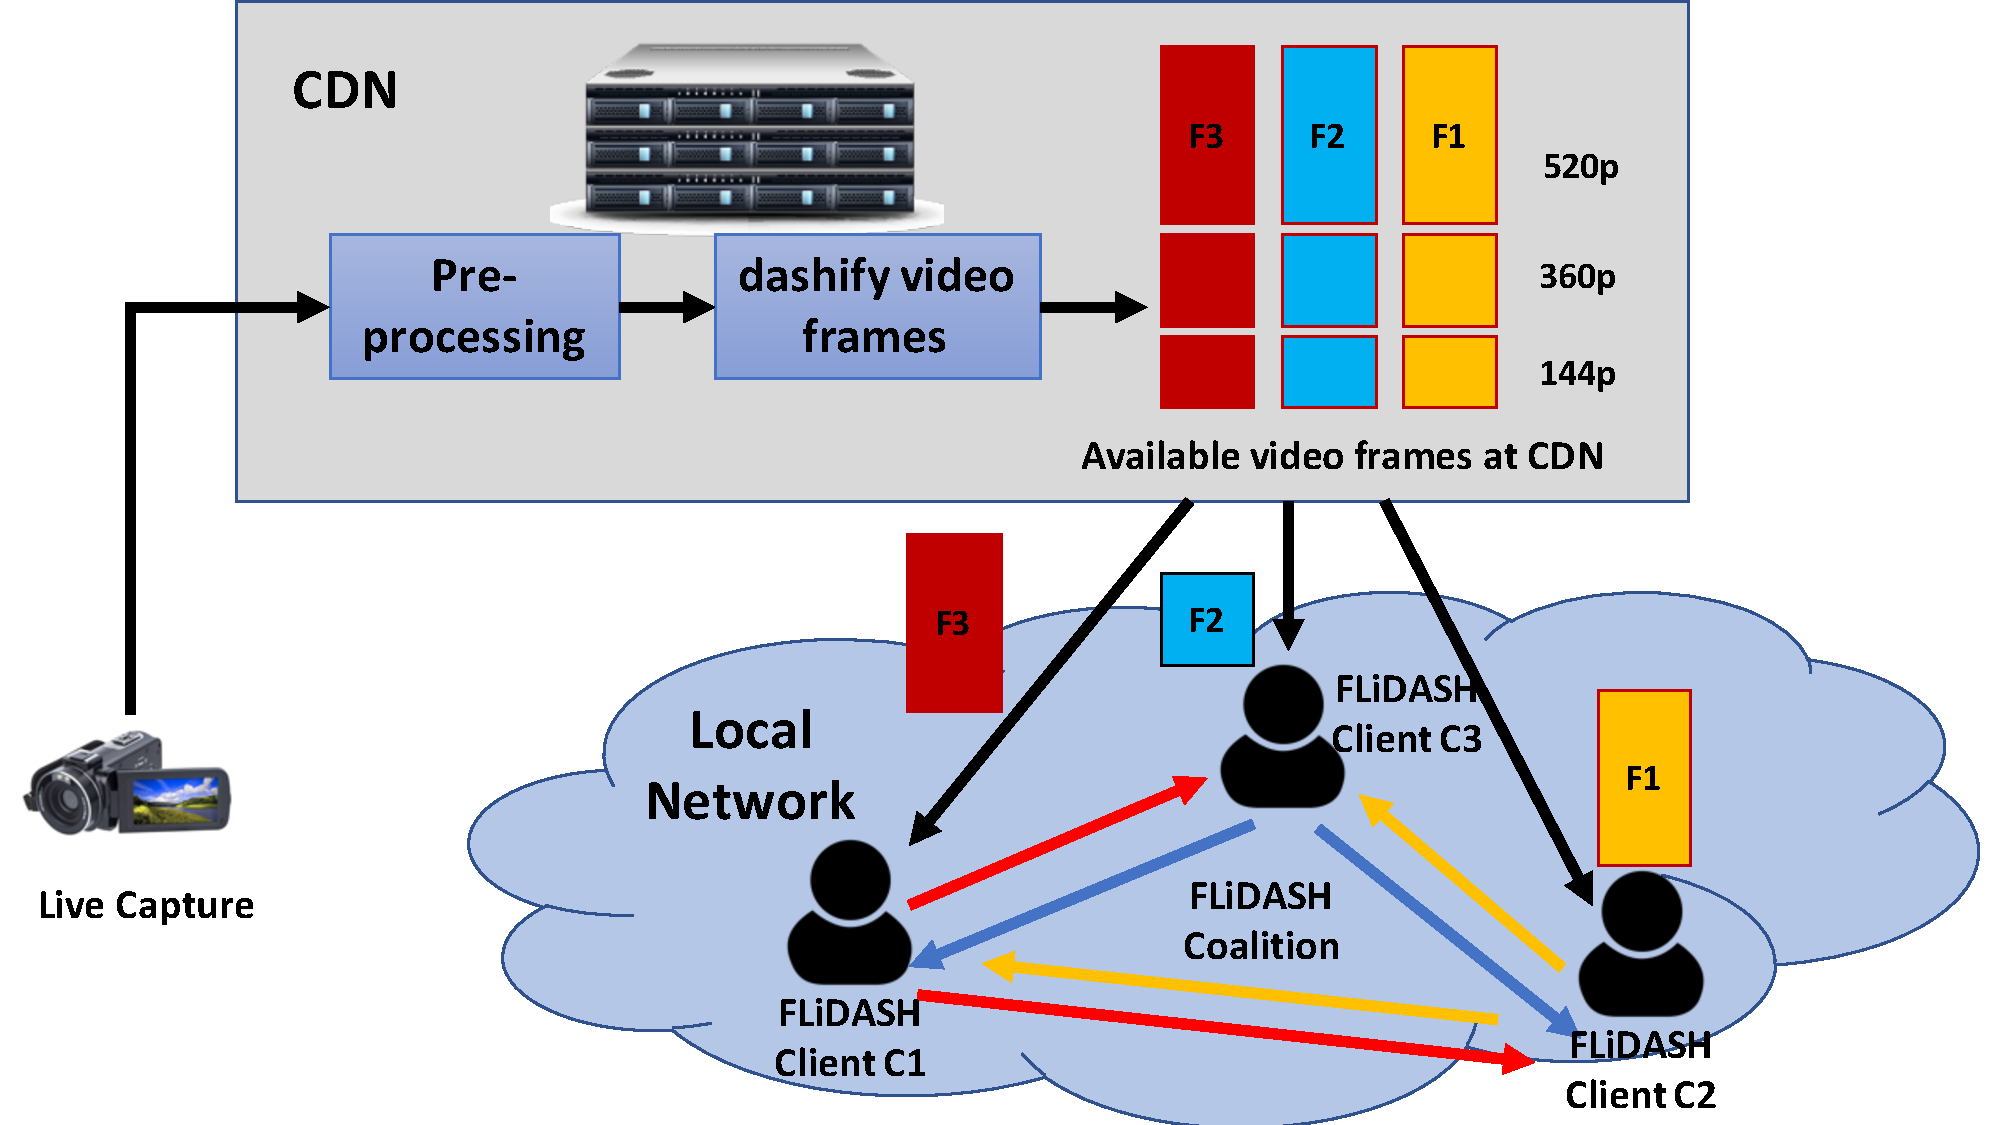
\includegraphics[width=0.8\linewidth]{img/flsd.pdf}
    \caption{Overview of \our: The clients under a local network create a coalition, every members of the coalition share the total download load.}
    \label{fig:chap06:flsd}
\end{figure}

However, developing such a system has multiple challenges. First, the coalition needs to be designed in a way such that downloading data directly from the content provider is costlier than sharing the data over the local network. Second, there should be a proper distribution of segment-wise data-download scheduling among the coalition members such that playback synchronization is not violated. A proper playback synchronization ensures that every player in the coalition should acquire the video segment $s_{i}$, either downloaded by itself or fetched from another coalition player through the direct local link, by the time it completes playing the previous video segment $s_{i-1}$; otherwise, there might be a rebuffering delay affecting the \ac{QoE}. Third, the Internet bandwidth of individual players may vary over time; therefore, the coalition as a whole should schedule the video segment downloads among its members as well as decide the bitrate of every video segment based on the \ac{ABR} principle.

Owing to the above challenges, we develop a coalition-based adaptive live streaming  called \textit{Federated Live Streaming over \ac{DASH}} (\our) where the streaming clients or players form a dynamic coalition based on the network quality parameters and collectively stream a live video. We use the playback buffer statistics at individual streaming clients to develop a distributed mechanism for coalition formation with the help from a proximity server (which can be an \ac{ALTO} server). The members of a coalition use a low-overhead gossip-based protocol for playback synchronization and takes following two decisions -- (1) scheduling the downloads of video segments among the coalition members based on their individual instantaneous network condition and the overall fairness criteria, and (2) bitrate of each video segments to optimize the overall \ac{QoE} of the coalition. We use the following \ac{QoE} objectives while making the above decisions -- (a) improve the overall video quality level, (b) improve the playback smoothness by reducing the quality fluctuations, (c) reduce rebuffering, and (d) improve fairness  among the coalition members in terms of the downloaded data share. We have implemented {\our} over an emulated environment and have thoroughly compared its performance with various other baselines. We observe that {\our} improves the overall \ac{QoE} with less traffic overhead at the backbone network.

The rest of the chapter is organized as follows. 

\subsection{Background of QUIC}

\begin{comment}
\subsection{Dynamic adaptive streaming over HTTP(DASH)}
DASH provides a standard solution for the efficient and easy streaming of multimedia using existing available HTTP infrastructure (particularly servers and CDNs, but also proxies, caches, etc.). DASH specification provides a full set of HTTP adaptive bitrate streaming features for delivering multimedia over Internet.The features include the following:\footnote{\url{https://www.wowza.com/forums/content.php?508-How-to-do-MPEG-DASH-streaming} (\lastaccessedtoday)}
\begin{itemize}
	\item Frame-synchronized adaptive bitrate switching.
	\item Codec-agnostic.
	\item DRM-agnostic. It specifically supports the Common Encryption (CENC) system.
	\item Evolving support for closed-captions and subtitles.
	\item Support for multiple file container formats.
	\item Support for multiple manifest formats for VOD and live streaming.
	\item Fast-growing industry support.
\end{itemize}

A DASH server provides client players with a list of the available media chunk URLs in a \textit{Media Presentation Description (MPD)} manifest file.

\end{comment}
%Today, the web is the most widely used service over the Internet where HTTP is used to transfer the content of a web page from the web server to the web client which is typically a browser.
%It serves pages to a client using application layer protocol HTTP.
%HTTP1.1~\cite{RFC2616} uses a request-response method, and almost each request requires a new TCP connection from the client to the server and vice versa.
%However, the current websites may require as many as $100$ objects to be fetched to render a page properly. If every HTTP request requires a new TCP connection,
%Therefore, a significant amount of time needs to be spent only on  TCP connection establishment. Further, most of the today's secure web-servers uses the TCP+TLS protocol stack (as shown in \fig\ref{fig:quic-protocolstack}), where {\em Transport Layer Security} (TLS) is used to establish the end-to-end secure tunnel between the server and the client. TLS needs one additional round trip time (RTT) for the server-client handshaking for security parameter exchange.
To solve the problems of connection setup and \ac{TLS} handshaking delay for every \ac{HTTP} request-response flow, Google introduced a new protocol in 2012, called  \acsu{SPDY}~\cite{SPDYingupweb,Erman} that can multiplex more than one \ac{HTTP} requests/responses into one \ac{TCP} connection. Although \acsu{SPDY} reduces the connection establishment time, however, due to \ac{TCP}'s in-order packet delivery, all the \ac{HTTP} streams in a multiplexed \ac{TCP} connection get blocked with \ac{SPDY} even for a single packet drop event from any one of the \ac{HTTP} streams, which is known as \ac{HoL} blocking problem. To address \ac{HoL} blocking, Google has introduced another new experimental protocol called \ac{QUIC}~\cite{roskind2015quic,Cui2017,Megyesi2016} that uses \ac{UDP} based multiplexed streaming to provide low latency connections for web access. As shown in \fig\ref{fig:quic-protocolstack}, \ac{QUIC} uses \ac{UDP} as the underlying transport layer protocol to solve the \ac{HoL} blocking issue with \acsu{SPDY}, and therefore it has its own congestion control and flow control mechanisms~\cite{Cui2017,roskind2015quic}. The key benefits of \ac{QUIC} over \ac{TCP}+\ac{TLS} are as follows -- (a) reduction in connection establishment latency, (b) multiplexing of multiple application flows without head-of-line blocking, (c) improved congestion control over multiplexed application flows, (d) forward error correction for low latency communication, and (e) connection migration to support seamless mobility in the network.

\begin{figure}[!t]
	\centering
	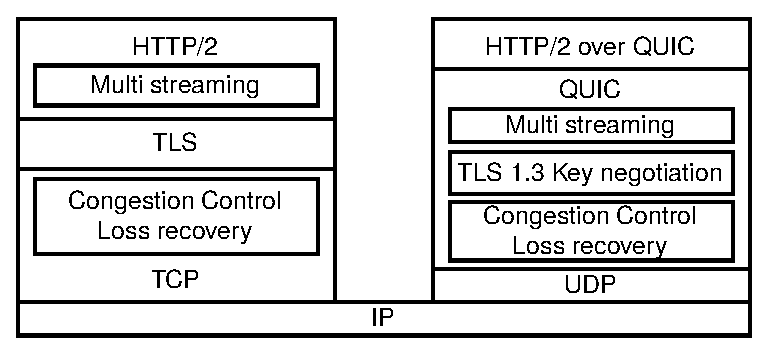
\includegraphics[width=0.7\linewidth]{img/quic-protocolstack}
	\caption{\acs{QUIC} Protocol Stack}
	\label{fig:quic-protocolstack}
\end{figure}

%\subsection{Quick UDP Internet Connections (QUIC):}

%It does not suffer from HoL blocking as it uses UDP as the transport protocol.
%As shown in \fig\ref{fig:quic-protocolstack}, unlike current TCP+TLS stack, QUIC does not require any separate TLS handshaking~\cite{Cui2017,roskind2015quic}. It can perform security handshaking during connection establishment only~\cite{Cui2017,Megyesi2016}. QUIC uses a congestion control algorithm similar to TCP, which are either TCP Reno, TCP New-Reno or TCP Cubic~\cite{Cui2017,roskind2015quic}.
%QUIC also uses a {\em forward error correction} (FEC) technique to reconstruct a lost packet in the network through redundant data transmission over multiple packets.
%This reconstruction is required to maintain QUIC philosophy of low latency connection. QUIC has been deployed in Google Chrome browser and Chromium browser.

Recent studies~\cite{Megyesi2016, Carlucci,Lychev2015,Biswal2016} on the performance of \ac{QUIC} have revealed that \ac{QUIC} can improve the web performance by reducing page load time even at poor network conditions.
%Next, we give a summary of the related works that have studied the performance of QUIC under various scenarios.
%Modern web run on top of TCP+TLS stack (\fig\ref{fig:quic-protocolstack}). This two stack have their own connection establishment time. As web need a lot of short-lived HTTP connections, this establishment time is huge part of their overall life time. To mitigate these problems, Google has developed QUIC.
%
%QUIC solves a number of transport-layer and application-layer problems including the one we mentioned earlier, experienced by modern web applications, while requiring little or no change from application writers. QUIC is very similar to TCP+TLS+HTTP2, but implemented on top of UDP. Having QUIC as a self-contained protocol allows innovations which are not possible with existing protocols as they are hampered by legacy clients and middleboxes.\footnote{\url{https://www.chromium.org/quic} (\lastaccessedtoday)}\\\\
%\noindent
%Key advantages of QUIC over TCP+TLS+HTTP2 include:
%\begin{itemize}
%	\item Connection establishment latency
%	\item Improved congestion control
%	\item Multiplexing without head-of-line blocking
%	\item Forward error correction
%	\item Connection migration
%\end{itemize}
%\begin{figure}
%    \centering
%    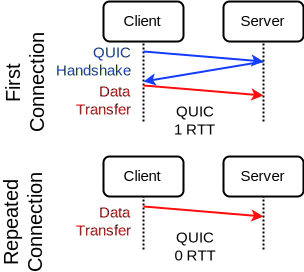
\includegraphics[width=0.7\linewidth]{img/quicrtt}
%    \caption{}
%    \label{fig:quicrtt}
%\end{figure}
%\subsection{Related Works}
%Most of the previous works in QUIC compare its performance with HTTP1.1 and SPDY~\cite{qian2015toward,Megyesi2016, Carlucci,Lychev2015,Biswal2016,bakri2015http}.
In \cite{Cui2017}, Cui \textit{et. al.} have shown that \ac{QUIC} has the potential to change the web and make it faster and more secure.
%as they have shown the improved performance of QUIC compared to various other end-to-end protocols.
Megyesi \textit{et al.}~\cite{Megyesi2016} have compared \ac{QUIC} with \acsu{SPDY} and \ac{HTTP} and found that \ac{QUIC} outperforms those protocols for web access under low network bandwidth availability. However, they have also noted that \ac{QUIC} does not work well with the large objects, such as large file transfer. In \cite{Biswal2016}, Biswal \textit{et al.} have found that \ac{QUIC} can load web pages much faster than HTTP2.0. They have also shown that \ac{QUIC}'s performance increases with increasing size of object and number of objects on a page, which is little contrary to the observation given by \cite{Megyesi2016}. Lychev \textit{et al.}~\cite{Lychev2015} have analyzed security aspects of QUIC and have presented the first security model for \ac{QUIC}. They have found that simple bit-flipping and replay attack can prevent \ac{QUIC} from achieving its goal of low latency. They have also claimed that this weakness is there because of the goal of low-latency. In~\cite{bakri2015http}, the authors have developed a service for multi-user virtual world by exploring the low latency features of HTTP2.0 and \ac{QUIC}.

In summary, most of these works claim that \ac{QUIC} has the proficiency to improve the performance of web access.
% As most of today's streaming services work on top of HTTP, like YouTube, NetFlix and so on,
Therefore, it would be interesting to see how web based video streaming services perform when the underlying \ac{TCP}+\ac{TLS} stack is replaced by \ac{QUIC}. However, to the best of our knowledge, no recent work has looked into web based adaptive streaming performance over \ac{QUIC}.
%In this paper, we investigate this performance issues by looking into a widely used streaming service, YouTube.

%Most of the work done on QUIC was how QUIC performs with respect to TCP and SPDY in terms of page load time. In \cite{citation-1-name-here} they studied about the performance of QUIC, SPDY and HTTP particularly about how they affect page load time. They found that none of these protocols is clearly better than the other two and the actual network conditions determine which protocol performs the best. Similarly in \cite{citation-6-name-here} they found out that QUIC reduces the overall page retrieval time with respect to HTTP in case of a channel without induced random losses and outperforms SPDY in the case of a lossy channel. The FEC module, when enabled, worsens the performance of QUIC.
%Almost all the research was concentrated on how QUIC performs in terms of page load time, the number of RTT's required and how it deals when there is packet loss so basically they were concerned about object transfers or static elements transfer and there were no major publications on how QUIC performs if it used for video streaming services like YouTube.

	
\subsection{Experiment Setup}
\label{sec:experiments}

In this subsection, we describe the testbed for monitoring video streaming traffic under various network conditions.
%Next, we describe the process for collecting video traffic data.

\subsubsection{Testbed}
Similar to the previous chapter, we have designed our testbed to observe streaming video traffic from YouTube. 
The monitoring is performed at the client end, where the video is played out in a browser.
Since we want to study the adaptation behavior when bandwidth changes, it is important that we can control the bandwidth available.
We do not have control over the available bandwidth to the YouTube server over the Internet, but we could place a bandwidth throttler that can restrict the bandwidth available to the client below what is actually available.
The complete testbed architecture is shown in \fig\ref{fig:experimentalSetup}.

\begin{figure}[!t]
	\centering
	
\includegraphics[width=0.7\linewidth]{img/experimentalSetup}
	\caption{Experimental testbed}
	\label{fig:experimentalSetup}
\end{figure}

The bandwidth throttler component is implemented using the {\tt NetFilterQueue} Linux library.
The {\tt iptables} tool, which uses {\tt NetFilterQueue}, is used to manipulate the network bandwidth available for the web browser.
%To simulate a given bandwidth, we delay the network packets before it reaches the application (browser).
Since we are comparing the performance of \ac{QUIC} and \ac{TCP}+\ac{TLS}, we need to play the videos at a browser which has support for both \ac{QUIC} and \ac{TCP}+\ac{TLS}. Google's Chrome browser supports both the protocol stacks that can be configured using {\tt chrome://flags}. We also use the command line tool \texttt{speedtest-cli} to periodically monitor the available network bandwidth at the backbone. If the backbone bandwidth drops more than $10$ Kbps from the current throttler bandwidth, we discard that data and initiate streaming of the corresponding video from the scratch.
%. Under this scenario, the streaming procedure for that video has been initiated again from the scratch.  

\subsubsection{Data Collection Process}
We use the {\tt NetMonitor} tool available as part of the browser developer tools to collect the traffic related information.
We focus on the \ac{HTTP} request-response messages, which are stored as \ac{HAR} file that contain information in \ac{JSON} format. In our data collection process, we start the bandwidth throttler before accessing a video for playback in a browser. We play the video till the end, while collecting the \ac{HAR} file containing the relevant traffic information.
The throttler is designed to switch bandwidth levels from $64$ Kbps to $1424$ Kbps in steps of $340$ Kbps at every $220$ seconds. Once the bandwidth reaches to $1424$ Kbps, the throttler starts decrementing the bandwidth at the same rate. 
%This is indeed a circular procedure that keeps on running at the background during the streaming of every video file. 
%The entire process is automated through a script. 
We use Google Chrome Remote Interface\footnote{\url{https://github.com/cyrus-and/chrome-remote-interface}} plugin to automatically open the browser and load a video.
To capture the \ac{HAR} files, we use \texttt{chrome-har-capturer}\footnote{\url{https://github.com/cyrus-and/chrome-har-capturer}} plugin.
Since \texttt{chrome-har-capturer} is not event driven, and must be configured to store a data for a fixed time window, we specify the video length with few additional minutes as the time to capture data. The length of the video can be found using YouTube video info \ac{API}\footnote{\url{http://www.youtube.com/get_video_info}}.
The additional wait also accounts for any rebuffering events when the video would stall.
%All these features allow in automatically playing large number of videos and capturing the data.

 
\begin{comment}
We want to test how YouTube performs with various network condition from the edge of the Internet. To do this, we set up our testbed as shown in \fig\ref{fig:experimentalSetup}. There are four components in our testbed. They are YouTube server, the Internet, bandwidth throttler and a QUIC supported browser. Although we do not have any control over the YouTube server, it is an essential part of the testbed as we are performing experiments on YouTube only.

To perform various experiment efficiently, we need a high-quality Internet connection. We do not want an Internet connection to be a bottleneck. It should support the speed we needed to perform the experiments. To ensure high-speed and high-quality Internet connection, we perform our experiments on the Institute's Internet backbone. Then again, we monitor the connection quality throughout the experiments.

As we want to perform experiments for various network conditions, we need to emulate those network conditions. To simulate the realistic bandwidth limited setting, we throttle the available link bandwidth. Linux system have a traffic shaper name {\fontfamily{qcr}\selectfont tc}. But there are some issue with {\fontfamily{qcr}\selectfont tc} for ongoing connections. So, we have designed our bandwidth throttler. There is a open Linux library, {\fontfamily{qcr}\selectfont NetFilterQueue}, available to perform various task on network packet from user space with the help of {\fontfamily{qcr}\selectfont iptables}. We took help of this tools to throttle bandwidth. In this tool, we hold packets in a queue and release them according to the required bandwidth.

\begin{figure}[h!]
\centering

\includegraphics[width=\linewidth]{img/experimentalSetup}
\caption{Experimental testbed}
\label{fig:experimentalSetup}
\end{figure}

As we are experimenting YouTube performance for the web, we need a browser. We want to compare YouTube's performance when it is using QUIC as underlying protocol with when it is using TCP+TLS as the underlying protocol. All the browsers support TCP+TLS, but there are only two browsers available which support QUIC as the underlying protocol. These are Chromium browser and Google Chrome browser. Both the browsers developed by Google only and they are almost identical in every aspect. However, Google Chrome is more popular than Chromium browser. So, we choose Google Chrome to perform the experiments. Both the browser have the option for enabling or disabling QUIC using {\fontfamily{qcr}\selectfont chrome://flags}. We perform experiments using both enabling the flag and disabling it for QUIC and TCP+TLS respectively.

Above mentioned details is the primary requirement for the experiments to be performed. However, we need to automate the process and collect relevant data out of these experiments. In following subsections, we discuss the data collection procedure and the automation procedure.


\subsection{Data Collection Procedure}
Almost all the popular browsers have developer tools. In this tool set, a user can perform various experiments on their website to observe a website performance. Among these tool set, one tool call {\fontfamily{qcr}\selectfont NetMonitor} (name of this tool is browser dependent). In this tool, one can see various information regarding HTTP request and response. These pieces of information are request and response headers and body, different time (like DNS lookup, connection establishment, waiting time before response arrives and time requires to receive the response). Most of the network tool have support for storing these pieces of information on the disk. It store those information in a format call HAR (\textbf{H}TTP \textbf{Ar}chive). HAR is JSON format, so it is easy to read by any text editor or programming language. In our experiments, we stored the HARs of each video and analyzed later.

For each experiment, we first run throttler program, then open a browser and loads the desired YouTube video. Then we waited till the video playback finishes. After completion of a video playback, we stored the HAR and closed the browser and throttler program. Throttler program not only throttle the bandwidth, but it also changes the bandwidth level. The bandwidth levels used are from 64 Kbps to 1424 Kbps, in a step of 340Kbps. Each level of bandwidth is kept fixed for 220 seconds. This whole procedure can be done manually. However, to collect data for a large number of videos, manual work can be very cumbersome and a waste of time. So, we automate the entire procedure.

\subsection{Automation procedure}
Automation is the one of the essential requirement to perform experiments. So, we have developed a python script which does all the step mentioned in the last subsection. For us, the major challenge in automation was automation of Google Chrome browser. To start Google Chrome browser and load the required video we use Google Chrome Remote Interface\footnote{\url{https://github.com/cyrus-and/chrome-remote-interface}} plugin. However, this plugin does not have access to the network monitor. So, to store HAR from network monitor of Google Chrome browser, we use chrome-har-capturer\footnote{\url{https://github.com/cyrus-and/chrome-har-capturer}} plugin. However, chrome-har-capture have a limitation. One can not trigger when to store HAR to disk. One has to give a waiting time at the very beginning, and this plugin will wait for that long before saving the HAR in the disk. So, we first find out the duration of the video using YouTube vide info api\footnote{\url{http://www.youtube.com/get_video_info}} then put waiting time as video length + 5 minutes. We have waited 5 minutes extra so the video can finish its playback even if playback stalls for rebuffering in between. We also turned off autoplay next feature of YouTube, so that it does not start playing some other video after completion of the desired video.

After automating all this, it becomes easier to run experiments for multiple videos unattended. In the following section, we discuss the different statistics of the videos and analysis parameters.


%As only Google Chrome browser and Chromium browser support QUIC, we need to perform experiments using one of them. Considering available plugins and APIs, there doesn't have any difference between Google Chrome browser and Chromium browser. So we choose Google Chrome browser to perform our experiment as it is more widely used over Chromium browser. To collect HAR from Google Chrome programmatically we use chrome-har-capturer\footnote{\url{https://github.com/cyrus-and/chrome-har-capturer}} and to automate this experiments we use Google Chrome Remote Interface\footnote{\url{https://github.com/cyrus-and/chrome-remote-interface}}.
%
%In order to simulate the  realistic bandwidth limited setting we throttle the available link bandwidth. Although Chrome support throttling in network monitor, there is no suitable way to change it from script. Therefore we make use of the throttler developed  with the Unix library {\fontfamily{qcr}\selectfont NetFilterQueue} \cite{citation-2-name-here}. It is a user-space library that provides an API to handle packets, which have been queued by the kernel packet filter, as per user requirement. Based on this library, traffic shaper was developed to control link bandwidth. However, we need to continuously monitor and ensure that the backbone network has sufficient bandwidth so that the overall link bandwidth is controlled only by the throttling procedure. We load a YouTube video, wait for the video to finish and then save the HAR and other information to the disk. During video playback, we also control network bandwidth by progressively increasing the bandwidth followed by a sudden decrease and the cycle repeats. The bandwidth levels used are from 64 Kbps to 1424 Kbps, in a step of 340Kbps. Each level of bandwidth is kept fixed for 220 seconds.
%
%\begin{figure}[h]
%	\centering
%	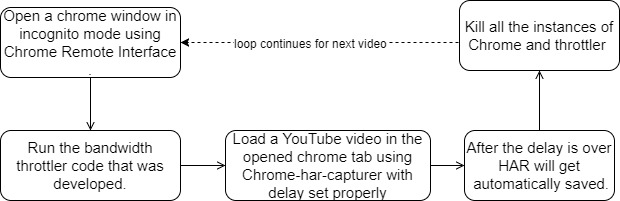
\includegraphics[width=\linewidth]{img/setup}
%	\caption{Experimental Set-up}
%	\label{fig:mesh11}
%\end{figure}
%
%\section{Dataset}
\end{comment}
\begin{comment}
\subsection{Extract Useful Information from the HTTP Headers}

From the HAR traces, we observe that YouTube uses a video playback request to grab the media data from the server. URLs for these video playback requests contain 35 parameters and their values:  \textit{pl, dur, expire, sver, gir, pcm2cms, mime, itag, signature, ipbits, source, keepalive, mt, mv, ms, mm, mn, key, clen, requiressl, lmt, initcwndbps, id, upn, sparams, fexp, ip, cpn, alr, ratebypass, c, cver, range, rn, and rbuf.} By close inspection of these parameters, we observe that the HTTP requests and responses are forwarded separately for the audio channel and the video channel. The value of the parameter \textit{mime} indicates whether the request is for audio channel or for video channel. Then, we figure out that the parameter \textit{itag} actually indicates the video quality for which a DASH request is made. YouTube samples every video under different video quality levels based on its resolution, bit rate and encoding techniques used for sampling, and assigns a numeric level to every quality, which is the itag value. The mapping between a particular \textit{itag} value and the corresponding video resolution, bit-rate and encoding parameters are given in \tbl\ref{table:2}.

\begin{table}[ht!]
	\centering
	\begin{tabular}{||c |c |c||} 
		\hline
		\textbf{Itag} & \textbf{Resolution} & \textbf{Type}  \\ [0.5ex] 
		\hline\hline
		160 & 256x144 & video/mp4 \\ 
		\hline
		278 & 256x144 & video/webm \\ 
		\hline
		133 & 426x240 & video/mp4 \\ 
		\hline
		242 & 426x240 & video/webm \\ 
		\hline
		134 & 640x360 & video/mp4 \\ 
		\hline
		243 & 640x360 & video/webm \\ 
		\hline
		135 & 854x428 & video/mp4 \\ 
		\hline
		244 & 854x428 & video/webm \\ 
		\hline
	\end{tabular}
	\caption{Information about itags}
	\label{table:2}
\end{table}

The behavior of these parameters under different scenarios like {\em Multiple videos multiple sessions, Single video multiple sessions, Single video single session} was observed. When a value does not change over multiple videos multiple sessions, then it indicates that the parameter does not take part in video adaptation procedure, and it basically forwards some static information, like the device and the operating system related information. If the value of a parameter changes for multiple video multiple sessions, but does not change for single video multiple sessions, then we can say that it is a video specific parameter.  If the value of a parameter changes for single video multiple sessions, but does not change for a single video single session even if the network quality changes, then we can say that it is session specific. The parameters that change only in this scenario when we change the link bandwidth, indicate that they possibly take part in the video adaptation process. From here, it was figured out in that  \textit{clen, dur, itag, lmt, mime, rbuf, rn, signature and range} are such parameters. However through close inspection, we find the parameters  \textit{mime} and  \textit{signature} relate to video channels, as we already discussed. Further the parameter  \textit{dur} denotes video duration, and it was observed that it changes only at microsecond order which is due to the change in video encoding technique. Consequently, we go for comparison of the other parameters between QUIC and TCP - \textit{ clen, itag, lmt, range, rbuf and rn.} It was observed that for the single video single session scenario, \textit{rbuf, rn} and \textit{range} change even for a single \textit{itag}. On the other hand, parameters like \textit{clen} change overall, but remain constant for a single \textit{itag} value.

\end{comment}
  
\subsection{Dataset and Parameters}
In this subsection, we give the details of the data collected to analyze YouTube adaptive streaming performance over QUIC. The complete dataset is available at \url{http://imdc.datcat.org/location/1-FWJR-3}. 
%\noteam{test2}

\subsubsection{Dataset}
   
%We wanted the bandwidth cycle to repeat at least once so we selected the videos that are on an average more than $30$ minutes in duration. The following table summaries the statistics about the data.

\begin{table}[t!]
    \centering
    \footnotesize
    \caption{Statistics of YouTube videos used in experiments. `\#' and 'Duration' indicate the number of videos and total playback duration, respectively.}
    \label{table:1}
    \begin{tabular}{| p{3cm} |l |p{2cm}|| p{3cm} |l |p{2cm}|} 
        \hline
        \textbf{Video Length (mins)} & \textbf{\#} & \textbf{Duration} & \textbf{Video Length (mins)} & \textbf{\#} & \textbf{Duration}  \\ [0.5ex] 
        \hline\hline
        $<$ 30 & 13 & 5h 59m & 30--40& 30 & 17h 08m\\ 
        \hline
        40--50 & 90 & 66h 09m & 50--60 & 31 & 27h 56m  \\ 
        \hline
        60--70 & 6 & 6h 29m &  $>$ 70 & 5 & 6h 11m\\ 
        \hline
    \end{tabular}
\end{table}

%\noteam{Other stat is almost done. I shall add it tomorrow evening.}

\begin{table}[!t]
    \centering
    \caption{\label{table:quality}Video categories with available levels and total durations. `fps' indicates frame per second.}
    \footnotesize
    \csvreader[tabular=|p{2cm}|p{1.5cm}|p{1.5cm}|p{3cm}|,
    separator=semicolon,
    %    table head=\hline Max Quality & Number of Video & Total Duration & Number of Quality Levels & Quality Levels\\\hline\hline,
    table head = \hline \textbf{Max Quality} & \textbf{Number of Videos} & \textbf{Total Duration} & \textbf{Number of Quality Levels}  \\\hline\hline,
    late after line=\\\hline]%
    {Chapters/03.DASH/Sec02/ytquic/csv/videocatagories.csv}{}%
    {\csvcoli&\csvcolii&\csvcoliii&\csvcolv}
\end{table}


With the setup described earlier, we have collected the HAR data for a total of $175$ videos for both QUIC and TCP. We have ensured that similar throttling behavior is applied during streaming over QUIC and streaming over TCP. The details of the video HAR data downloaded using this procedure have been summarized in \tbl\ref{table:1}. These videos can be further categorized using the best (maximum) quality and the number of quality levels available on YouTube, as shown in \tbl\ref{table:quality}. However, we do not observe all these different quality levels during the video playback, as it depends on the YouTube streaming quality adaptation algorithm based on available channel condition during the playback as well as on the playback screen resolution. We have performed these experiments with standard definition display without full screen mode. Therefore we observe maximum playback quality of 480p even if the video supports 1080p high definition (HD) rendering. 
%HD streaming requires very hing bandwidth at the network backbone, and it was difficult to get that bandwidth continuously during the experiment phase. However, the observed behaviors are sufficiently generalized, because we can get video bit-rate adaptation with at least $4$ different quality levels for most of the videos.     

%We can categorize the videos we played in our experiments in eight different categories based on the best quality of a video available on YouTube. In \tbl\ref{table:quality} give a detailed view of different categories.

%From \tbl\ref{table:quality}, we can see that we have used broad categories of videos regarding quality and bitrate. A total number of quality levels depend on maximum quality available for a video. In general, frame rate for a video is 30fps (frame per second). However, there are other options for high-definition (HD) videos. HD video can be 60fps or 50fps also. But they always have the 30fps option. In the case of a full HD (1080p) video have a higher frame rate, HD (720p) version also have the higher frame rate.

%Although most of the videos we played in our experiments have higher quality options, actual playback quality depends on the playback screen resolution. As we performed these experiments with standard HD (720p) display without full-screen mode, playback quality never goes beyond 480p. It is a way; YouTube saves viewers' bandwidth. It downloads the quality it can render on the viewing screen.

\subsubsection{Parameters Considered}
Similar to the previous chapter, From the HAR traces, we observe that YouTube uses a video playback request to grab the media data from the server. URLs for these video requests contain several parameters and their values~\cite{mondal2017youtube}. From these parameters, we found that three parameters \textit{itag}, \textit{range} and  \textit{rbuf} provide adaptive streaming performance related information which are useful for our analysis. %The details of these parameters are as follows. 
%We will not discuss how we conclude these parameters are related to DASH for space contraint. \noteam{We can refer our NOSSDAV paper here} We are going to describe each of these parameter here.

%\begin{table}[t!]
%	\centering
%	\footnotesize
%	\caption{Information about \textit{itag} values. The quality parameter indicates the quality level indicator for a resolution.}
%	\label{table:itag}
%	\begin{tabular}{|c|c||c|c||c|c|} 
%		\hline
%		\textbf{Quality} & \textbf{Resolution} & \textbf{Type} & \textbf{itag} & \textbf{Type} & \textbf{itag}  \\ [0.5ex] 
%		\hline\hline 
%		144p & 256x144 & mp4 & 160 & webm & 278\\ 
%		\hline
%		240p & 426x240 & mp4 & 133 & webm & 242\\
%		\hline
%		360p & 640x360 & mp4 & 134 & webm & 243\\
%		\hline
%	    480p & 854x480 & mp4 & 135 & webm & 244\\
%		\hline
%	\end{tabular}
%\end{table}
%
%
%\textbf{\textit{itag}:} It is a numeric value to identify the type of media. It defines codec, resolution, frame rate and type of the media. It can be noted that YouTube uses separate connections for audio and video, and therefore the type of the media can be either audio or video. Here we analyze the video streaming behavior. Although there is a large number of \textit{itag}s\footnote{\url{http://www.genyoutube.net/formats-resolution-youtube-videos.html}} supported by YouTube, we found a handful of them in our experiment which are supported by browsers, as listed in \tbl\ref{table:itag}.
%
%%\subsubsection{\textit{clen}} From our observation, we understand that \textit{clen} is the content length of a specific media with a specific \textit{itag} for a video in the number of bytes. It varies only with video and \textit{itag}.
%
%\textbf{\textit{range:}} The range parameter provides the byte range of the requested video segment. Apart from video quality, YouTube also adapts this parameter based on available channel quality~\cite{mondal2017youtube,anorga2017analysis}. If the channel quality is good, YouTube downloads data at a larger video segment by increasing the range values. 
% The \textit{range} values have two integers separated by a dash (-). The first integer is always smaller than the second one, and therefore we can say that these two integers are the \textit{start} and \textit{end} of the \textit{range} values. It behaves like range parameter in HTTP request header. It was concluded that range defines the byte range of the video for a \textit{itag} value that the client requests from the server. YouTube client adaptively changes this parameter to increase or to decrease the video chunk size to download, based on network conditions.

%\textbf{\textit{rbuf}:} \textit{rbuf} is the receive buffer occupancy at the client side~\cite{anorga2017analysis}. This gives an indication of the streaming performance as well as video quality of experience (QoE) performance in terms of rebuffering counts. When \textit{rbuf} becomes zero, the streaming client initiates a rebuffering of data which reduces the video QoE. A larger value of \textit{rbuf} indicates better video quality for YouTube. 
%The initial observations indicate that \textit{rbuf} grows as the YouTube client fetches more data from the server. However, with a close inspection of the HTTP request messages, we observe that the value of \textit{rbuf} decreases if there is no request from the client to the server. Further, whenever \textit{rbuf} starts decreasing, the client starts fetching data for a different \textit{itag} value (as we observe near lower bandwidth ranges).

%\subsubsection{\textit{rn}} It is a non-decreasing parameter for a session. It does not depend on any other parameter. By observing the sequence of HTTP requests sent by the YouTube client to YouTube server, we can conclude that \textit{rn} is the request number to identify a DASH video playback request uniquely.

%URLs for these video playback requests contain 35 parameters and their values:  \textit{pl, dur, expire, sver, gir, pcm2cms, mime, itag, signature, ipbits, source, keepalive, mt, mv, ms, mm, mn, key, clen, requiressl, lmt, initcwndbps, id, upn, sparams, fexp, ip, cpn, alr, ratebypass, c, cver, range, rn, and rbuf.} By close inspection of these parameters, we observe that the HTTP requests and responses are forwarded separately for the audio channel and the video channel. The value of the parameter \textit{mime} indicates whether the request is for audio channel or for video channel. Then, we figure out that the parameter \textit{itag} actually indicates the video quality for which a DASH request is made. YouTube samples every video under different video quality levels based on its resolution, bit rate and encoding techniques used for sampling, and assigns a numeric level to every quality, which is the itag value. The mapping between a particular \textit{itag} value and the corresponding video resolution, bit-rate and encoding parameters are given in \tbl\ref{table:itag}.

%The behavior of these parameters under different scenarios like {\em Multiple videos multiple sessions, Single video multiple sessions, Single video single session} was observed. When a value does not change over multiple videos multiple sessions, then it indicates that the parameter does not take part in video adaptation procedure, and it basically forwards some static information, like the device and the operating system related information. If the value of a parameter changes for multiple video multiple sessions, but does not change for single video multiple sessions, then we can say that it is a video specific parameter.  If the value of a parameter changes for single video multiple sessions, but does not change for a single video single session even if the network quality changes, then we can say that it is session specific. The parameters that change only in this scenario when we change the link bandwidth, indicate that they possibly take part in the video adaptation process. From here, it was figured out in that  \textit{clen, dur, itag, lmt, mime, rbuf, rn, signature and range} are such parameters. However through close inspection, we find the parameters  \textit{mime} and  \textit{signature} relate to video channels, as we already discussed. Further the parameter  \textit{dur} denotes video duration, and it was observed that it changes only at microsecond order which is due to the change in video encoding technique. Consequently, we go for comparison of the other parameters between QUIC and TCP - \textit{ clen, itag, lmt, range, rbuf and rn.} It was observed that for the single video single session scenario, \textit{rbuf, rn} and \textit{range} change even for a single \textit{itag}. On the other hand, parameters like \textit{clen} change overall, but remain constant for a single \textit{itag} value.

\subsection{Performance Comparison}
%We evaluate QUIC's performance over the standard TCP+TLS stack for adaptive video streaming by playing 175 video clips from YouTube in our testbed. 
For performance comparison between adaptive streaming over \ac{QUIC} and adaptive streaming over \ac{TCP}, we focus on two performance metrics -- (a) video \ac{QoE}, and (b) data download and data wasted due to quality switching. 
%In this section, at first, we evaluate Google's claims about the QUIC by comparing it with normal TCP connection.  After that, we compare data wastage while playing video for the normal TCP based connection and the QUIC based connection.

\subsubsection{Does QUIC Improve Video QoE?}
%Here we compare four different QoE metric of video streaming network standard TCP+TLS stack and QUIC stack. These metrics are i) number of quality switches, ii) overall playback quality (bitrate), iii) rebuffering count and iv) data wastages.
%After playing all the videos in both TCP+TLS stack and QUIC stack, we have first analyzed the following three different performance metrics to check how the streaming performance differs for the two protocol stacks.   
We quantify video quality using three parameters which impact \ac{QoE}~\cite{balachandran2012quest}.
\begin{enumerate}[leftmargin=*]
	\item\textbf{Video Quality Switches:} For adaptive video streaming, the streaming client dynamically adapts the video quality based on the environment (like available channel bandwidth). If the number of quality switching is high, then it negatively impacts the video QoE. 
	\item\textbf{Playback Quality:} We measure what proportion of the video that is played at the highest possible bitrate. 
	\item\textbf{Rebuffering Events:} We measure the number of times the playback buffer is completely used up and triggers rebuffering.
\end{enumerate}
%As mentioned in~\cite{balachandran2012quest}, these three metrics give a good indication of QoE for video streaming applications. 

\subsubsection{Video Quality Switch}
\begin{figure}[!t]
    \captionsetup[subfigure]{}
    \begin{center}
%        \subfloat[\label{fig:reschange_up}Quality Improvements]{
%            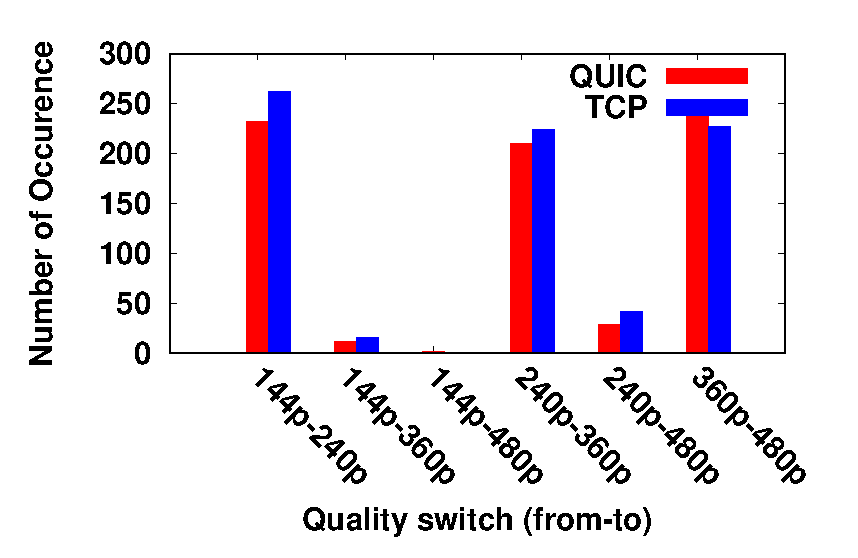
\includegraphics[width=0.48\linewidth]{img/metric/reschange_up}
%        }
%        \subfloat[\label{fig:reschange_down}Quality Drops]{
%            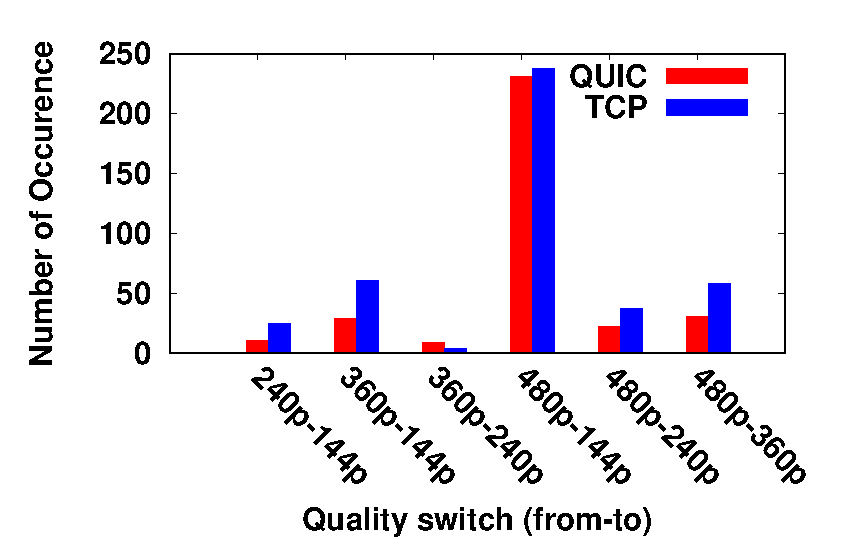
\includegraphics[width=0.48\linewidth]{img/metric/reschange_down}
%        }
        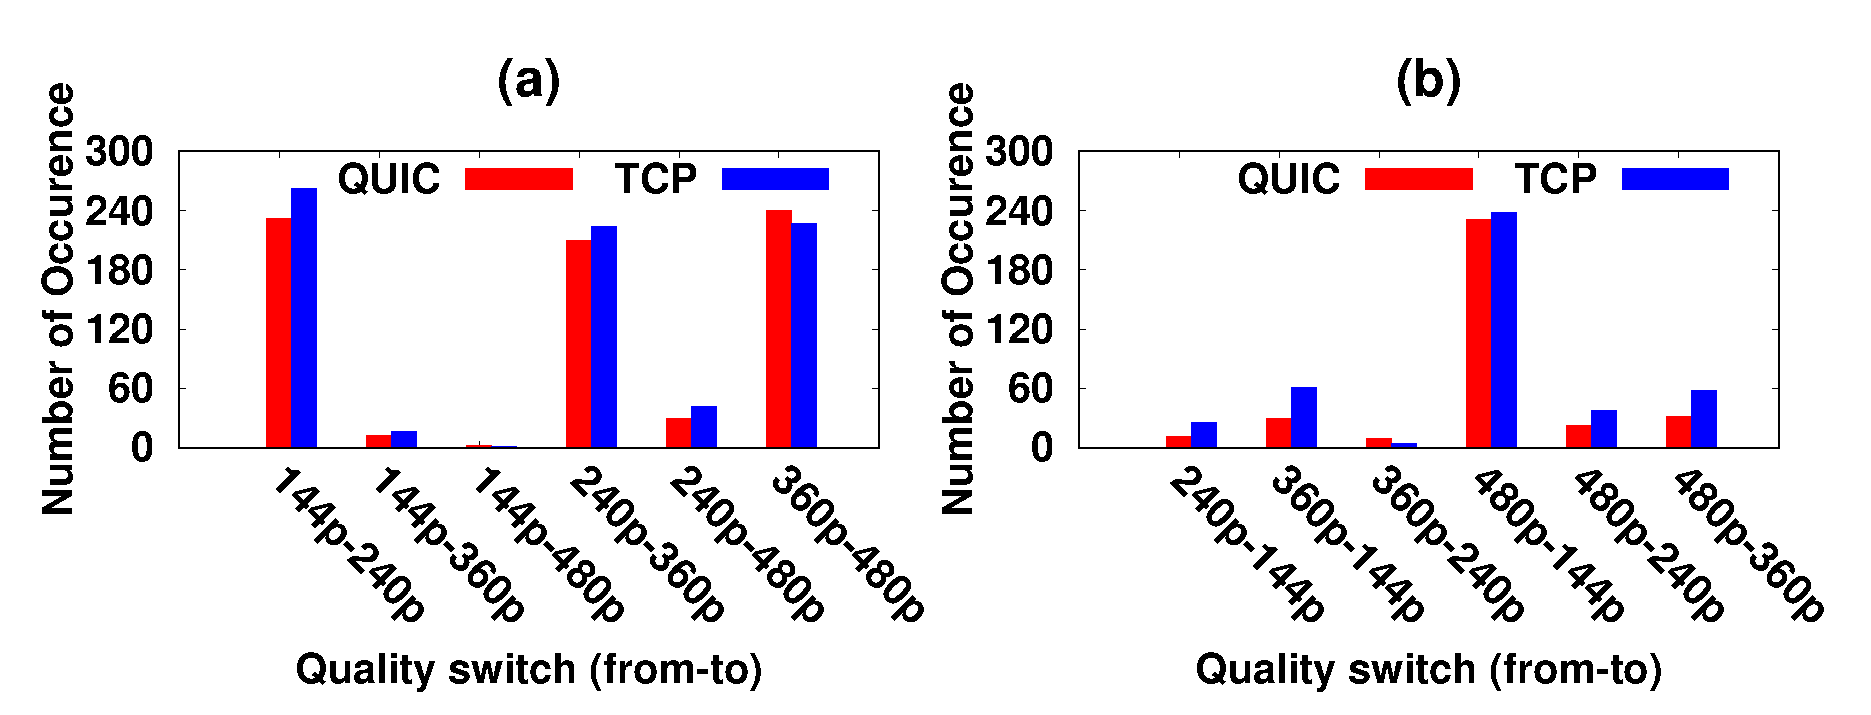
\includegraphics[width=0.9\linewidth]{img/plotdata/metric/reschange_up_down}
        \caption{\label{fig:reschange}Quality switching: (a) Quality upgrade, (b) Quality drop}
    \end{center}
\end{figure}

%\begin{figure}[!t]
%    \captionsetup[subfigure]{}
%    \begin{center}
%%        \subfloat[\label{fig:reschange_up_percent}Quality Improvements]{
%%            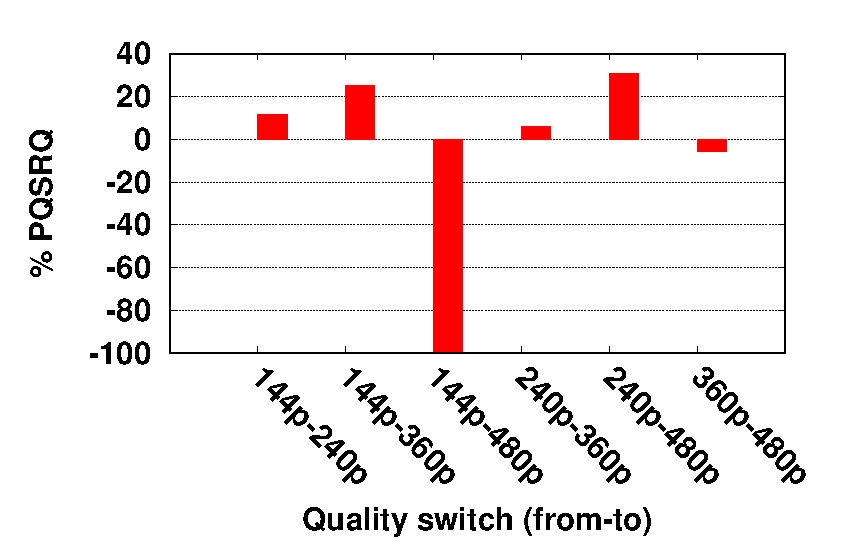
\includegraphics[width=0.48\linewidth]{img/metric/reschange_up_percent}
%%        }
%%        \subfloat[\label{fig:reschange_down_percent}Quality Drops]{
%%            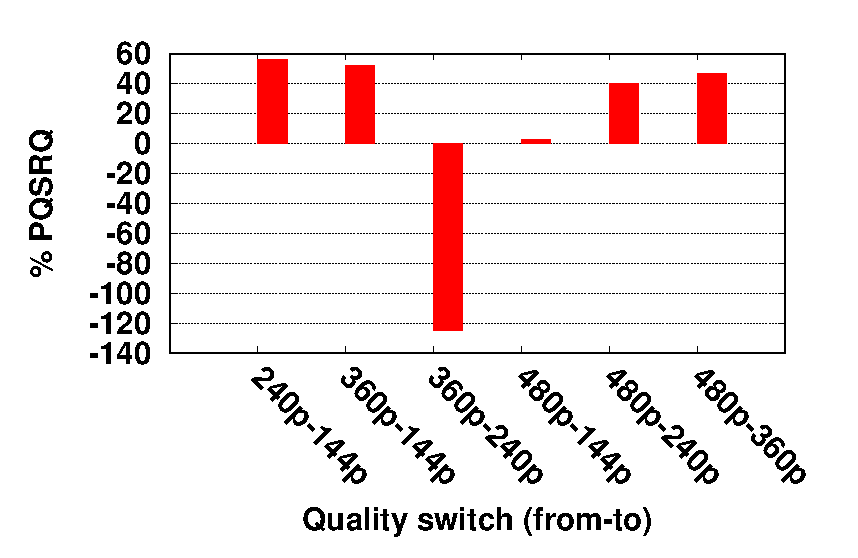
\includegraphics[width=0.48\linewidth]{img/metric/reschange_down_percent}
%%        }
%        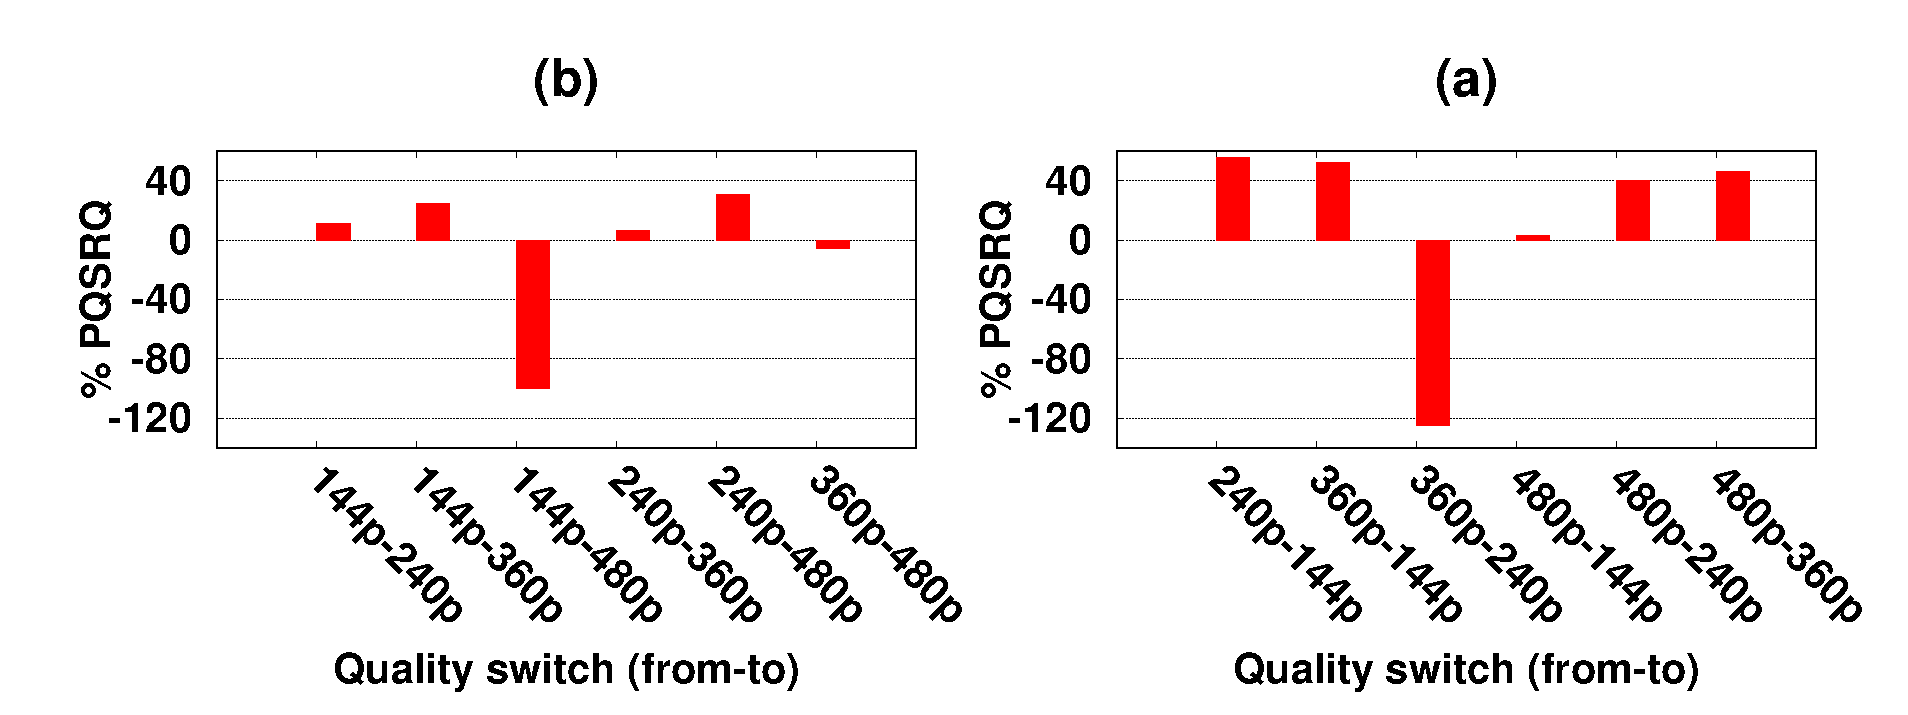
\includegraphics[width=\linewidth]{img/plotdata/metric/reschange_up_down_percent}
%        \caption{\label{fig:reschange_percent}Percentage quality switch reduction with QUIC: (a) Quality upgrade, (b) Quality drop}
%    \end{center}
%\end{figure}

We compare the number of switches in video quality, both in terms of quality upgrades and quality drops, as shown in \fig\ref{fig:reschange}.
We observe that \ac{QUIC} incurs less quality switches than that of \ac{TCP} for almost all the cases. 
%To quantify the improvement in quality switching with QUIC, we define a metric called \textit{Percentage Quality Switch Reduction with QUIC} (PQSRQ) which is defined as follows. For two quality levels $\mathcal{Q}_1$ and $\mathcal{Q}_2$, let $QSQ(\mathcal{Q}_1,\mathcal{Q}_2)$ and and $QST(\mathcal{Q}_1,\mathcal{Q}_2)$ denote the number of quality switch from $\mathcal{Q}_1$ to $\mathcal{Q}_2$ with QUIC and TCP, respectively.  Then, $PQSRQ(\mathcal{Q}_1,\mathcal{Q}_2) = \frac{QSQ(\mathcal{Q}_1,\mathcal{Q}_2)}{QST(\mathcal{Q}_1,\mathcal{Q}_2)} \times 100\%$. \fig\ref{fig:reschange_percent} plots the value of PQSRQ for various quality levels, both during quality improvements and quality drops. We observe that 
It is evident from the figure that for some quality levels, the percentage reduction in quality switches is more than $20\%$ during quality upgrades, and more than $40\%$ during quality drops. For the few cases when \ac{QUIC} performs worse than \ac{TCP}, we actually note that the number of data points for those quality levels is less in our collected dataset. Interestingly, in terms of percentage quality switch reduction, \ac{QUIC} outperforms \ac{TCP}  more during quality drops compared to quality upgrades, which is an indication of good \ac{QoE}.  Nevertheless, it is expected that the overall playback quality should be biased towards the high quality video segments for supporting better viewing experiences to the end users, which we explore next. 

\subsubsection{Video Quality During Playback}
%\begin{figure}[!t]
%    \centering
%    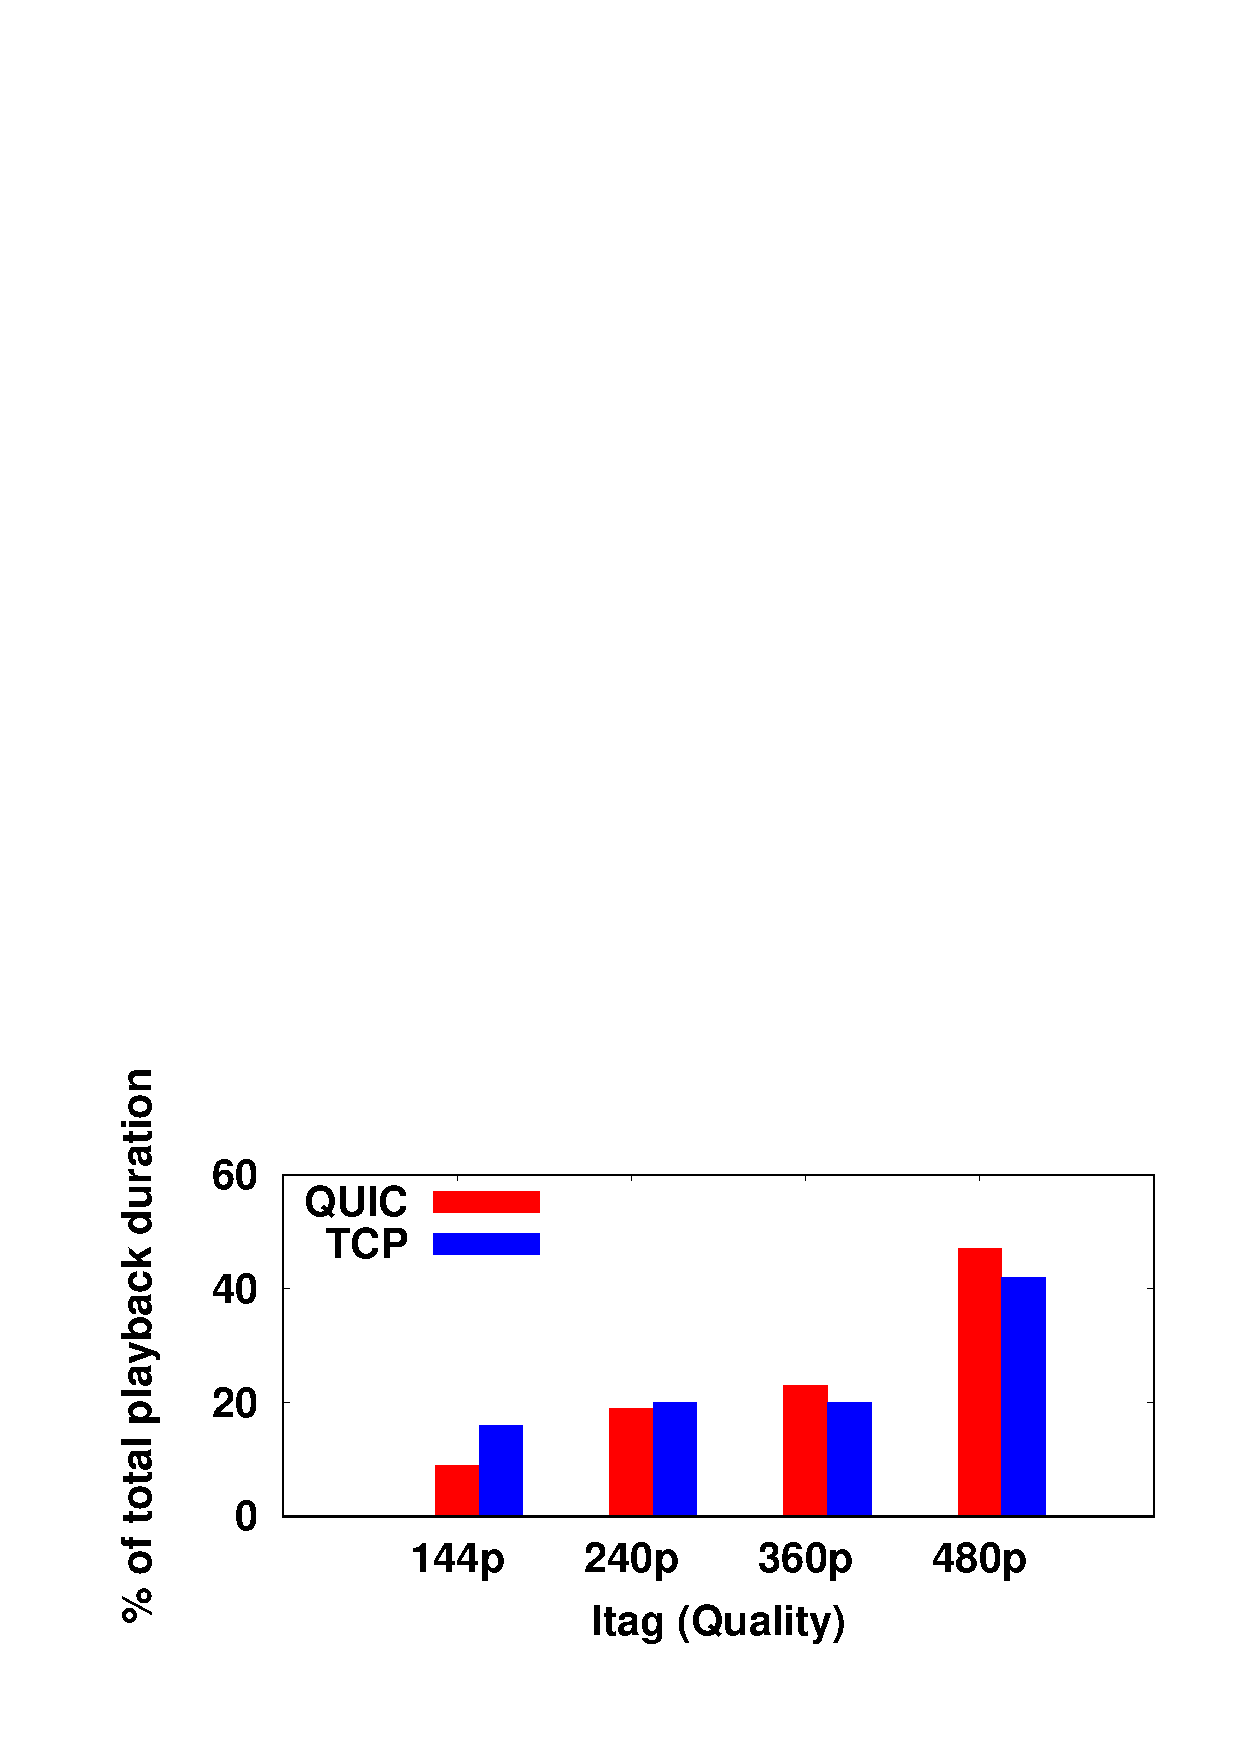
\includegraphics[width=\linewidth]{img/metric/time_duration_percent}
%    \caption{Overall playback Time of Each Quality \notesc{convert this to percentage - (data downloaded for a particular quality / total data downloaded for all the qualities) x 100\%} \noteam{Done.}}
%    \label{fig:avg_bitrate}
%\end{figure}

\begin{figure}[!t]
	\captionsetup[subfigure]{}
	\begin{center}
%		\subfloat[\label{fig:avg_bitrate}\% Playback Time]{
%			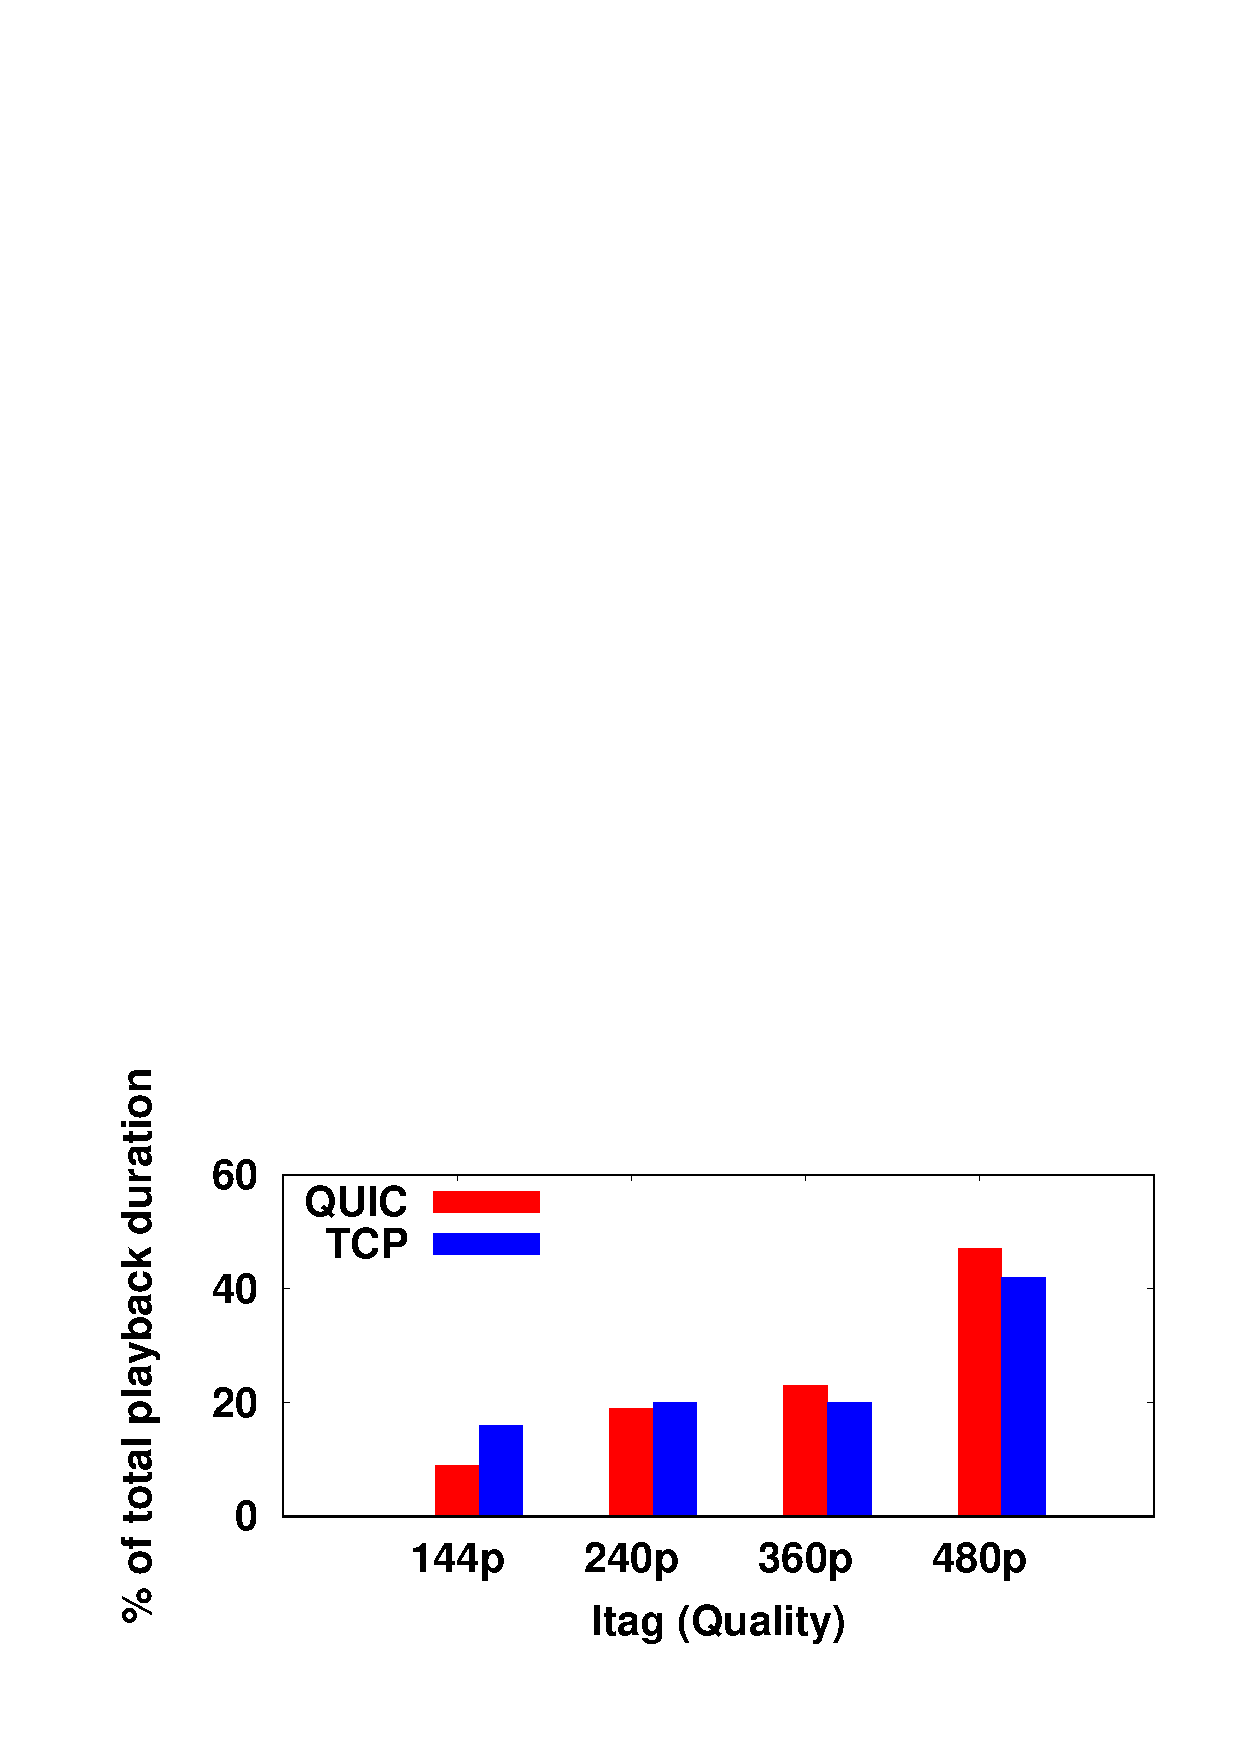
\includegraphics[width=0.48\linewidth]{img/metric/time_duration_percent}
%		}
%		\subfloat[\label{fig:rebuffering}Rebuffering Count]{
%			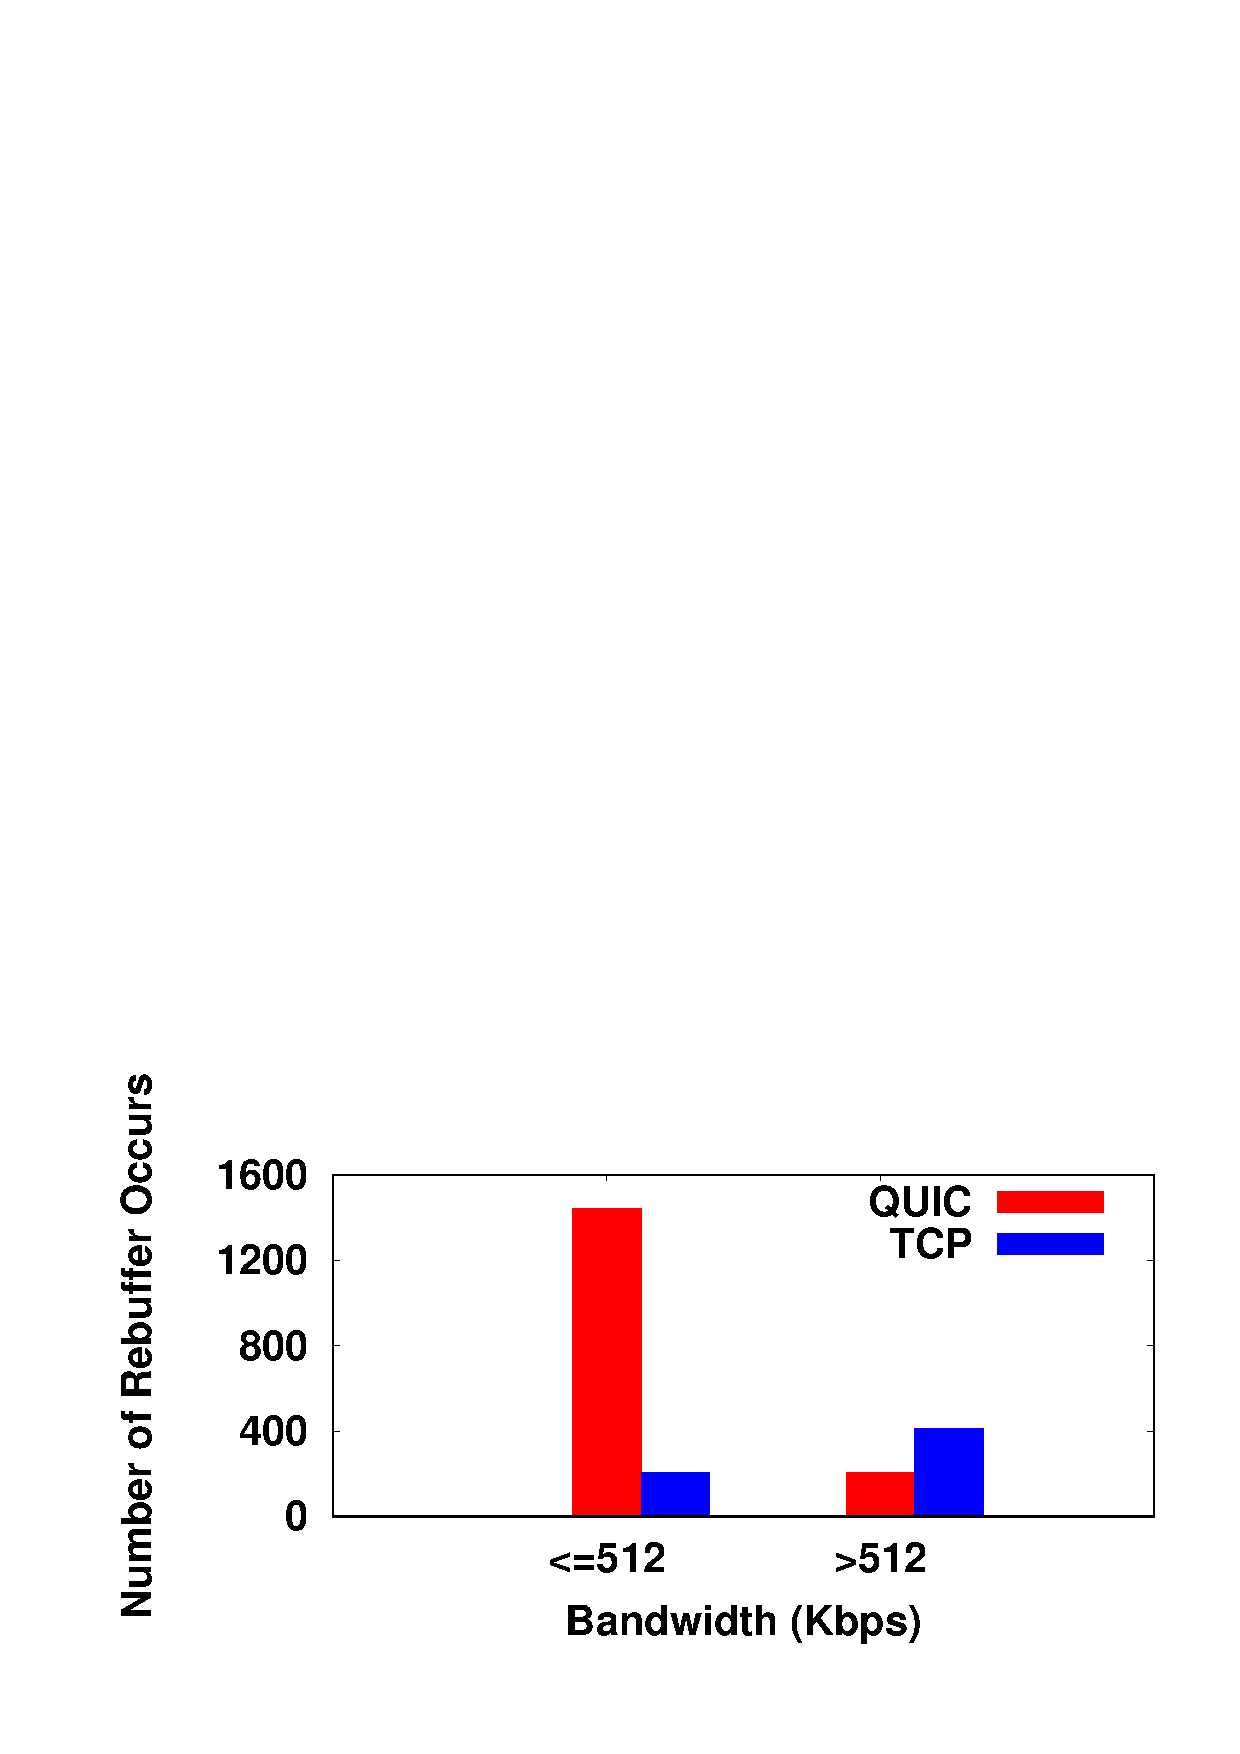
\includegraphics[width=0.48\linewidth]{img/metric/rebuffering}
%		}
        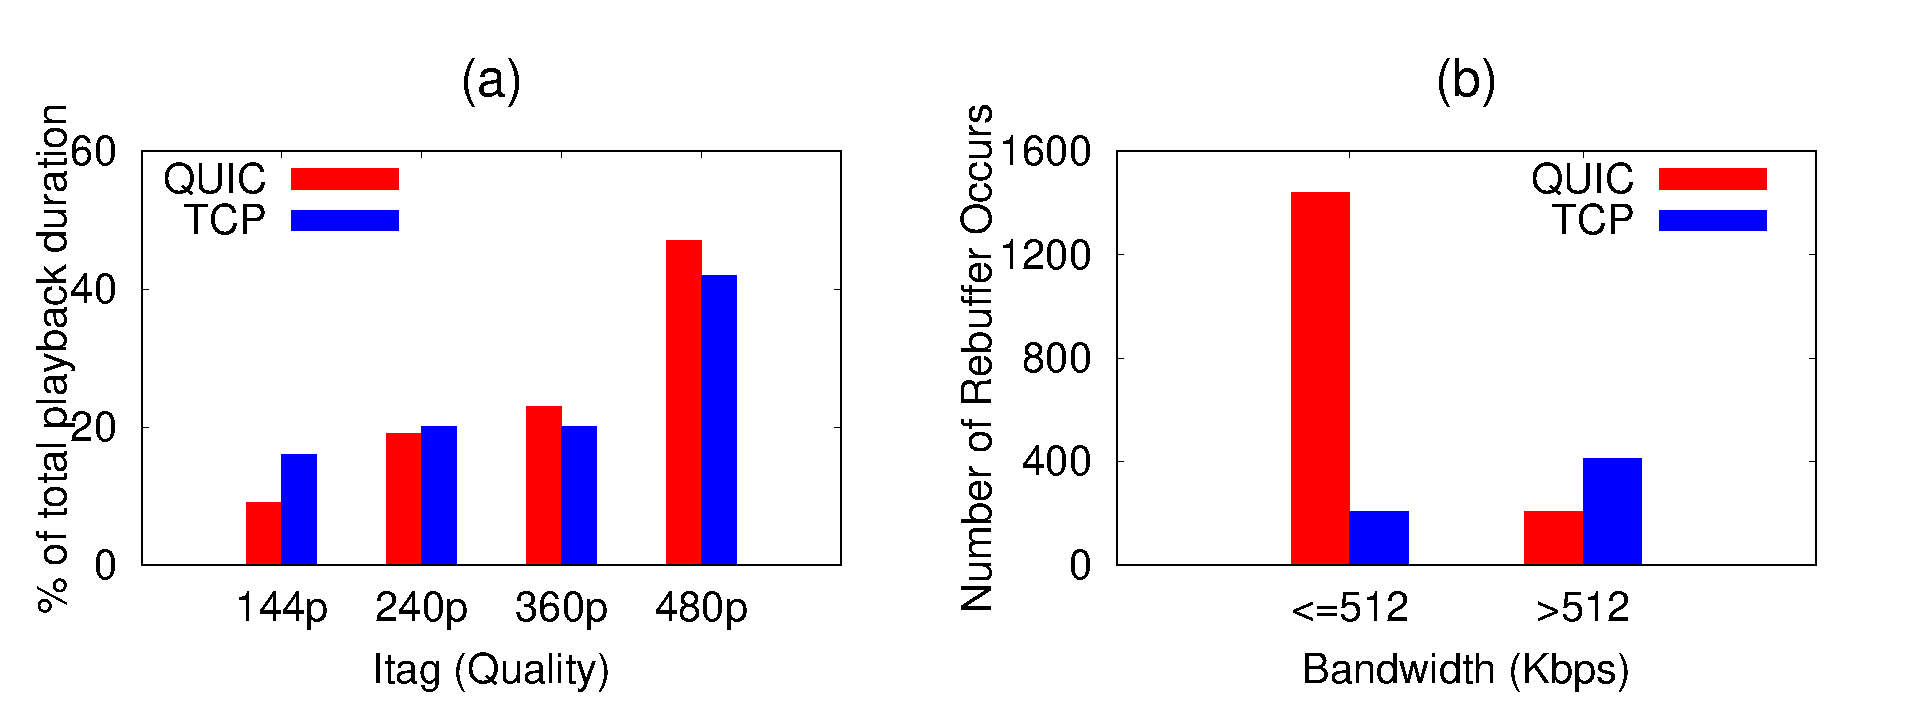
\includegraphics[width=0.9\linewidth]{img/plotdata/metric/time_duration_percent_rebuffering}
		\caption{\label{fig:bitrate_rebuffering}(a) Overall playback time,  (b) Rebuffering}
	\end{center}
\end{figure}

We investigate how long does a video play at a different video quality levels.
\fig\ref{fig:bitrate_rebuffering}(a) shows the percentage of total playback time at each video quality. 
Note that under similar experiment conditions, \ac{QUIC} enabled player plays the video at higher resolution compared to \ac{TCP}. Therefore, it provides better \ac{QoE} compared to \ac{TCP} for adaptive streaming in terms of quality switching and overall playback quality. 

%We compare the total playback time for streaming over QUIC and streaming over TCP, and we observe that QUIC is biased towards the high quality video segments. It can be noted here that during the data collection phase, we have ensured that a video should experience similar bandwidth throttling with respect to time ($\pm 10 Kbps$ deviation with respect to time, as mentioned earlier), when downloaded through both QUIC and TCP. Therefore, \fig\ref{fig:avg_bitrate} and \fig\ref{fig:reschange} together ensure that while QUIC reduces switching between video qualities, it tends to download video segments with higher quality values under the similar network bandwidth availability. Therefore, it provides better QoE compared to TCP for adaptive streaming in terms of quality switching and overall playback quality. 


\subsubsection{Rebuffering}
%\begin{figure}[h!]
%\centering
%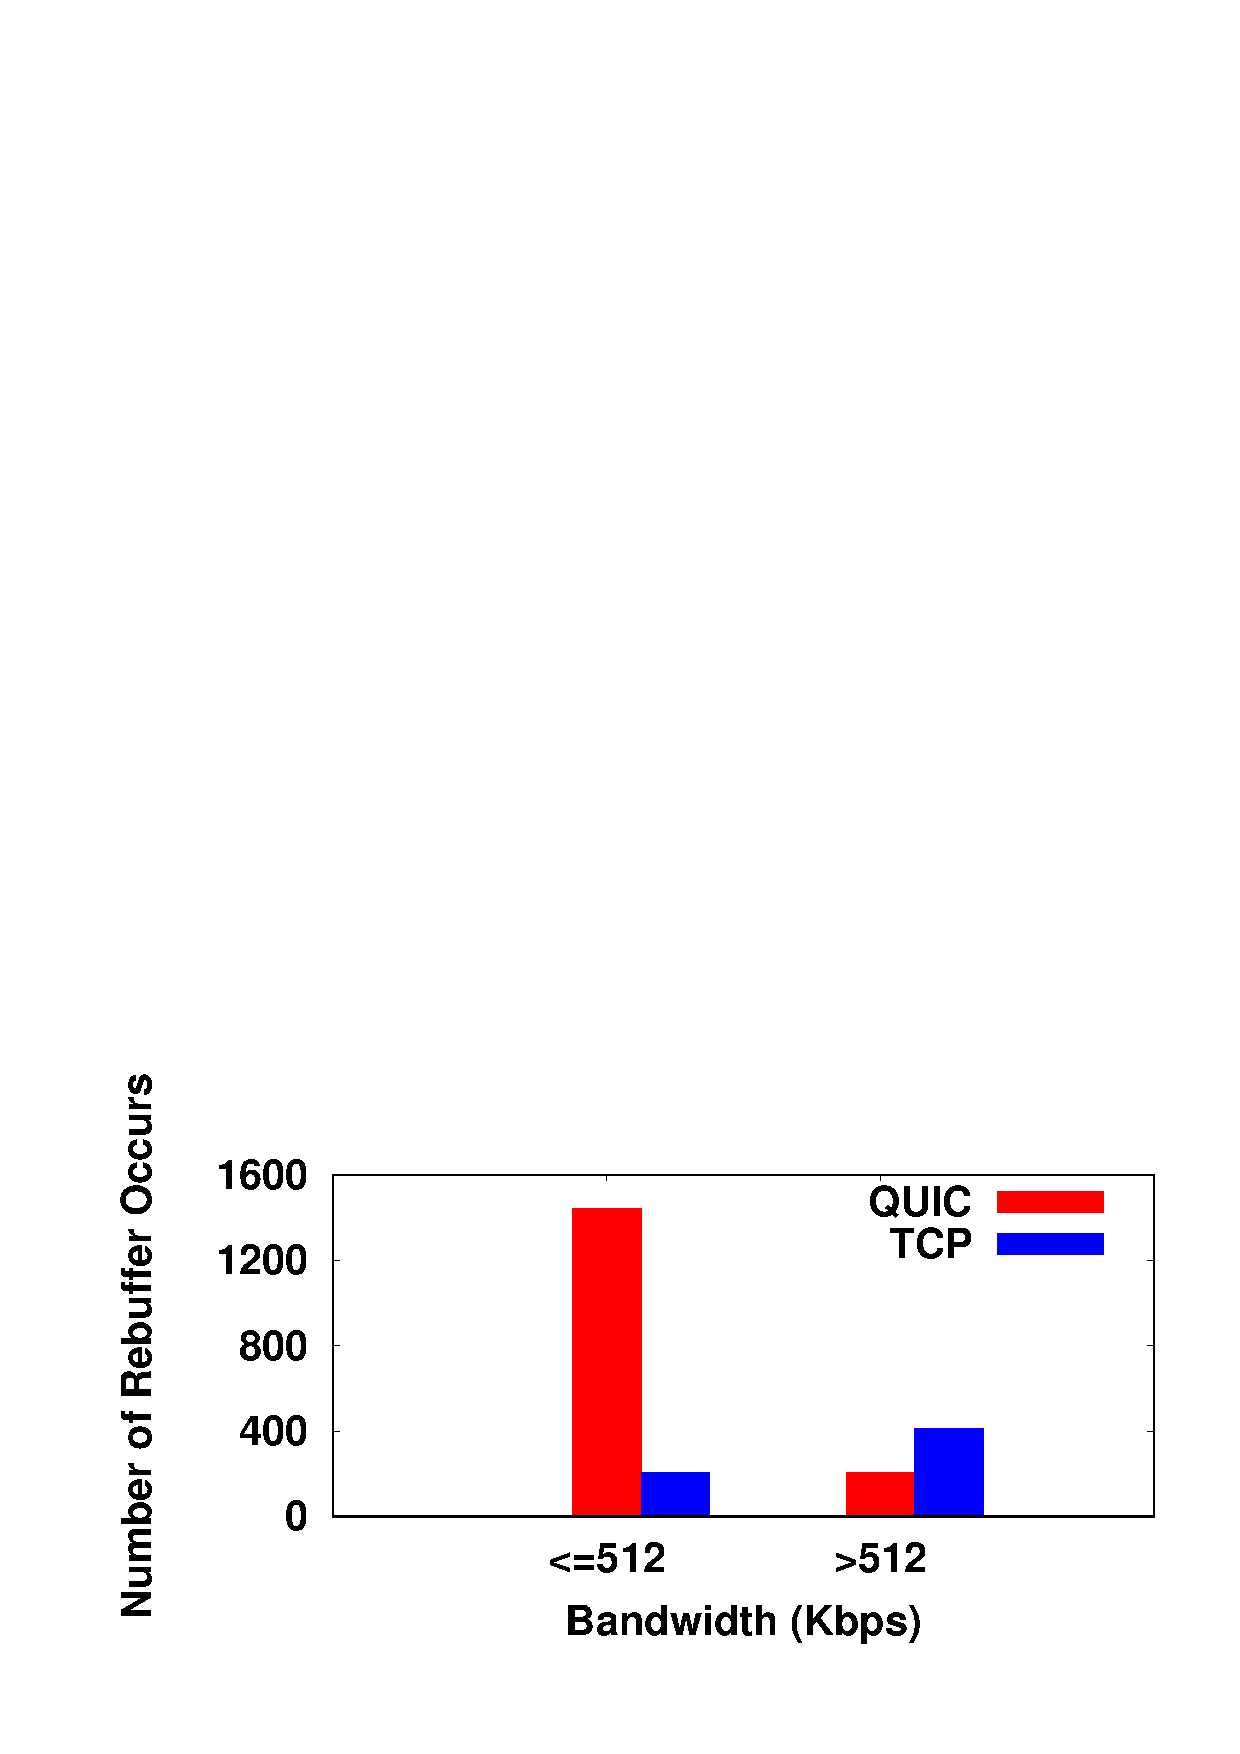
\includegraphics[width=\linewidth]{img/metric/rebuffering}
%\caption{Rebuffering Count in Different Bandwidth Levels \notesc{Show two scenarios -- (a) bandwidth less than 512 Kbps and (b) bandwidth greater than 512 Kbps}\noteam{Done.}}
%\label{fig:rebuffering}
%\end{figure}

%\begin{table}[h!]
%    \centering
%    \caption{Rebuffering}
%    \label{table:rebuffering}
%    \begin{tabular}{||c|c|c|}
%        \hline
%        Bandwidth & QUIC & TCP \\\hline\hline
%        64 & 1236 & 205 \\\hline
%        404 & 206 & 0 \\\hline
%        744 & 0 & 0 \\\hline
%        1084 & 0 & 0 \\\hline
%        1424 & 206 & 410 \\\hline
%        Total & 1648 & 615 \\\hline
%    \end{tabular}
%\end{table} 

We counted the number of rebuffering events during playback for both \ac{QUIC} and \ac{TCP} enabled streaming.
We used two bandwidth settings: (a) low bandwidth at less than 512 Kbps, (b) high bandwidth at greater than 512 Kbps.
\fig\ref{fig:bitrate_rebuffering}(b) shows the frequency of rebuffering events.
When the channel bandwidth is less than $512$ Kbps, QUIC shows runs out of buffered data more frequently than TCP. 
Since QUIC tries to maintain a high video quality, therefore, even at low bandwidth it does not quickly switch to a low bitrate leading to buffer depletion and triggers rebuffering.

%Next we observe another important and critical QoE metric, which is rebuffering count. During a rebuffering event, the streaming client's playback buffer becomes zero, and the video rendering halts at this point, resulting in poor QoE. As rebuffering depends on the available channel bandwidth along with current playback quality, we plot total rebuffering counts over all the dataset for two different bandwidth levels -- (a) channel bandwidth less than  $512$ Kbps and (b) channel bandwidth greater than $512$ Kbps. The resultant plot is shown in \fig\ref{fig:rebuffering}. We have interesting observation here. When the channel bandwidth is less than $512$ Kbps, QUIC shows significantly higher numbers of rebuffering events compared to TCP. On contrary, with channel bandwidth more than $512$ Kbps, QUIC performs better than TCP. So, in terms of rebuffering, we can say that QUIC performs poorly compared to TCP when channel quality is bad. Incidentally, we observe that QUIC tries to download high quality videos even at low bandwidth availability, which we presume as one of the reasons for the large number of rebuffering events.  

In summary, we observe that although \ac{QUIC} tries to download high quality videos even at low bandwidth availability and reduces number of quality switches during adaptive streaming, it can significantly increase the rebuffering events when video quality if low. 
If this rebuffering count goes beyond a threshold, \ac{QoE} for the video streaming application may suffer. 
As the rebuffering count during the video streaming over \ac{QUIC} is significantly higher than that of \ac{TCP}, when channel quality is poor, we conclude that \ac{QUIC} may not improve overall video \ac{QoE} under all conditions. 

%
%Rebuffering is the most critical QoE metric for video streaming. Before the age of dynamic adaptation begins, rebuffering was the only QoE metric. So, we also compared rebuffering count in the \fig\ref{fig:rebuffering} and the \tbl\ref{table:rebuffering}. We found that QUIC rebuffers more for lower bandwidth. It happens because QUIC tries to higher quality for longer playback time. However, TCP is more conservative than QUIC. So, QUIC does not perform well enough here.

\subsection{Impact of ABR Streaming over Data Consumption: QUIC vs TCP}

%Adaptive video streaming improves QoE by dynamically adapting video quality levels based on available channel bandwidth, however it has a direct implication of the amount of data that is downloaded at the client side. 
Existing studies on adaptive video streaming has shown that the complete data, which is downloaded by the streaming media client, is not utilized during the actual video playback~\cite{krishnappa2013dashing}. 
%A significant amount of data is wasted during the quality adaptation, as the streaming clients use a conservative approach during quality switching. 
In this section, we discuss the performance of adaptive streaming over \ac{QUIC} and \ac{TCP} in terms of data consumption. 

\begin{figure}[!t]
	\captionsetup[subfigure]{}
	\begin{center}
%		\subfloat[\label{fig:down_quality} At Different Quality]{
%			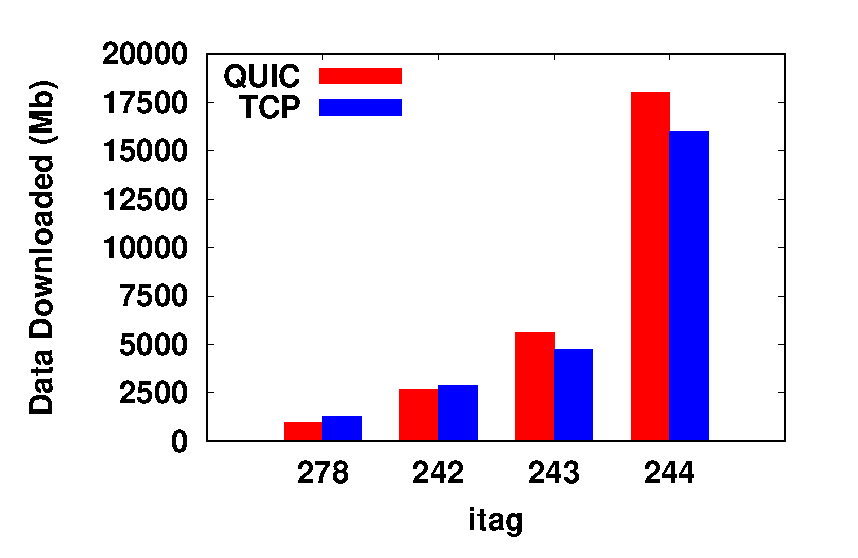
\includegraphics[width=0.48\linewidth]{img/CDF/Data_Dowloaded}
%		}
%		\subfloat[\label{fig:down_band}At Different Bandwidth]{
%			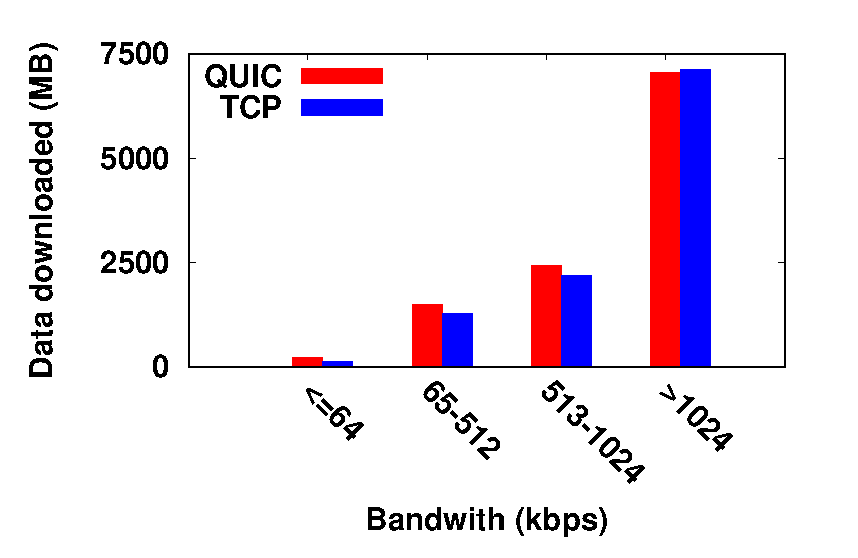
\includegraphics[width=0.48\linewidth]{img/CDF/data_downloaded_bw}
%		}
        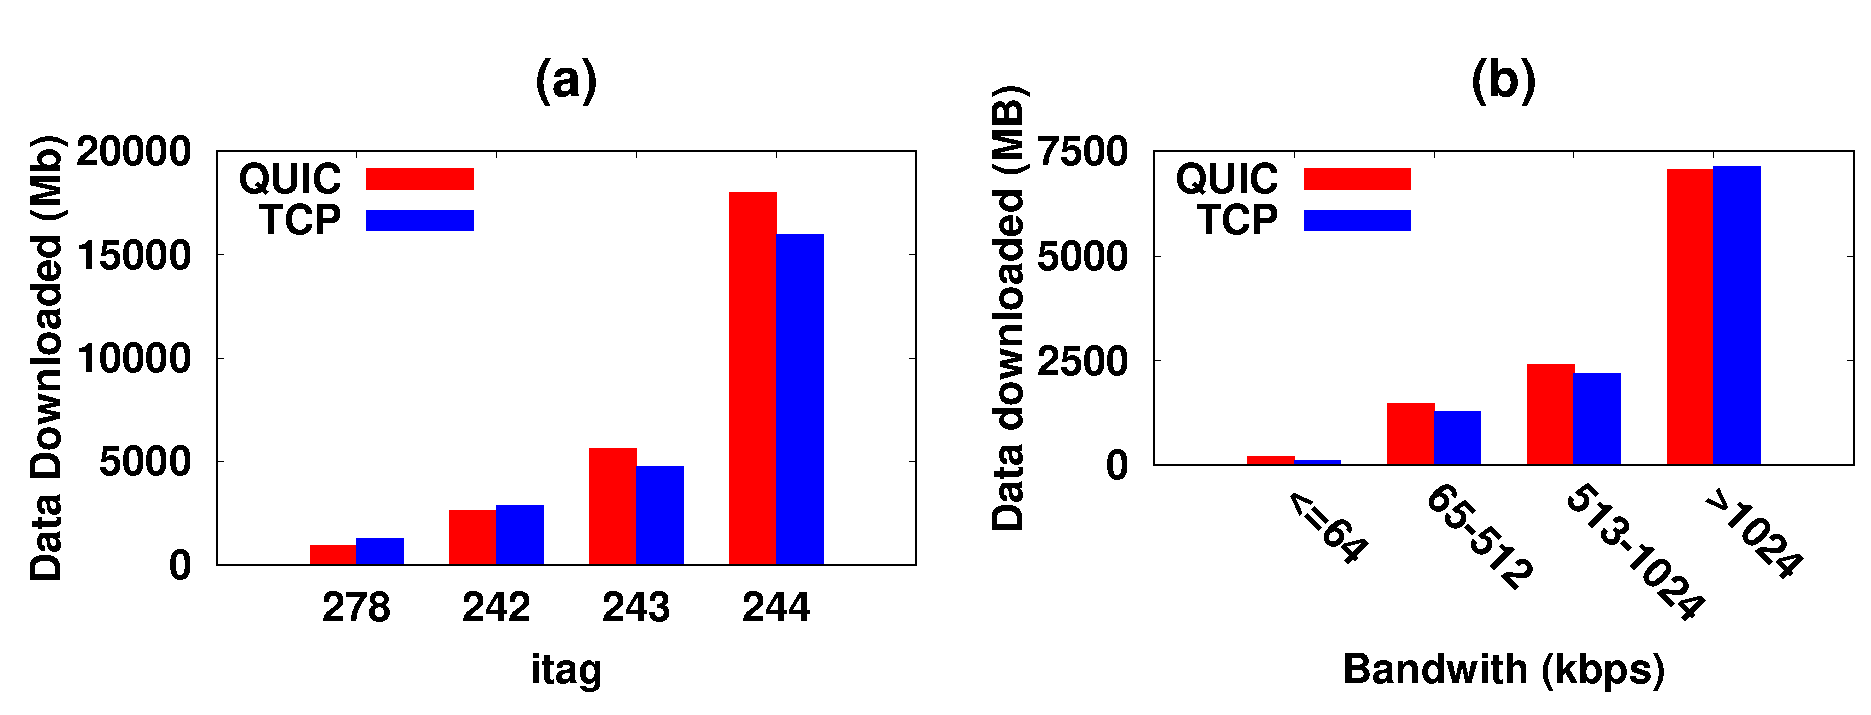
\includegraphics[width=0.9\linewidth]{img/plotdata/CDF/downloaded/data_dowloaded_itag_bw}
		\caption{\label{fig:data_download}Data downloaded: (a) Different quality levels, (b) Different channel bandwidth}
	\end{center}
\end{figure}


\subsubsection{Data Download for Adaptive Video Streaming}
We first look into the total data downloaded with \ac{QUIC} and \ac{TCP} during the playback of same set of videos under similar channel conditions. \fig\ref{fig:data_download}(a) shows the total data downloaded for different quality levels, and \fig\ref{fig:data_download}(b) plots the total data downloaded under various channel conditions in terms of bandwidth availability. We observe that \ac{QUIC} downloads more data under itag value $243$ and $244$ which are the best quality levels observed in the collected data set. 
%We then look into the total data download under various network conditions (channel bandwidth availability). \fig\ref{fig:down_band} plots the total amount of data downloaded over all the sampled videos grouped into four different available bandwidth conditions. 
Further, the figure indicates that the total data downloaded with \ac{QUIC} is high compared to \ac{TCP} when the available channel bandwidth is less than $1$ Mbps. Therefore, we hypothesize that with \ac{QUIC} enabled YouTube streaming can download high quality videos even at the low network quality. 
However, as we mentioned earlier, there is a possibility of data wastage during the quality switching with adaptive video streaming over the web. Next, we first explain the reason for this data wastage, and then we go for a thorough analysis of the data wastage for the two protocols. 

%Let us look at the total data downloaded (\fig\ref{fig:rabuf761856q}) by QUIC and TCP and the data wasted (\fig\ref{fig:rabuf76q1}) by both the protocols. Data wasted is computed by considering the fact that if there is lower resolution data when a higher resolution is being played then the lower resolution data is being wasted. The amount of data downloaded and data wasted has been calculated using the bit rates available for each itag in the HAR files.

%\begin{figure}[ht!]
%	\centering
%	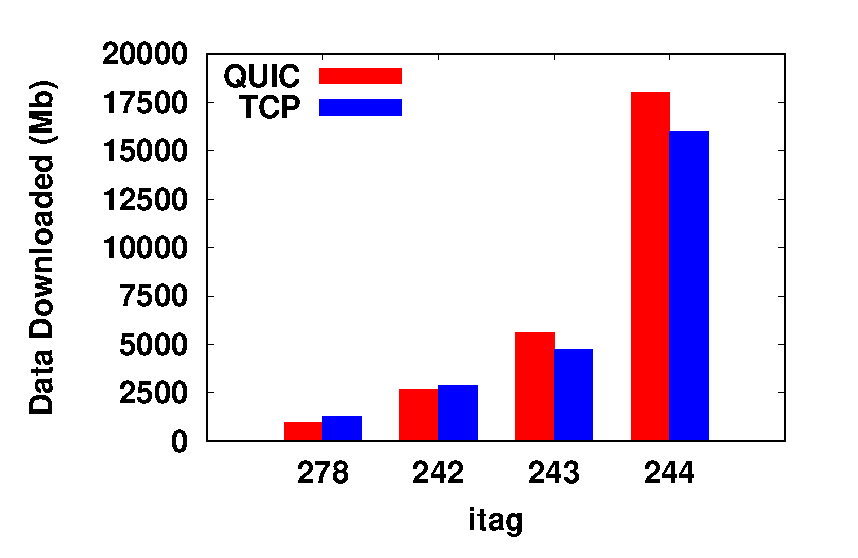
\includegraphics[width=0.9\linewidth]{img/CDF/Data_Dowloaded}
%	\caption{Amount of Data Downloaded}
%	\label{fig:rabuf761856q}
%\end{figure}


%\notesc{Total data downloaded at various bandwidth buckets --  (a) $\leq 64$ Kbps, (b) $65-512$ Kbps, (c) $513-1024$ Kbps, (d) $> 1024$ Kbps}

\subsubsection{Why There is a Possibility of Data Waste During Adaptive Streaming?}


%\begin{figure}[!t]
%	\captionsetup[subfigure]{}
%	\begin{center}
%		\subfloat[\label{fig:rseg1Q}QUIC]{
%			\includegraphics[width=0.48\linewidth]{img/QUICPlots/plot_timerange}
%		}
%		\subfloat[\label{fig:rsegr1T}TCP]{
%			\includegraphics[width=0.48\linewidth]{img/TCPPlots/plot_timerange}
%		}
%		
%		\caption{\label{fig:rserr1}Plot for \textit{Time Range} over time for a YouTube video of id $<$OJZgOOOE1zY$>$ \notesc{The fonts need to be clear}}
%	\end{center}
%\end{figure}
\begin{figure}[!t]
\centering
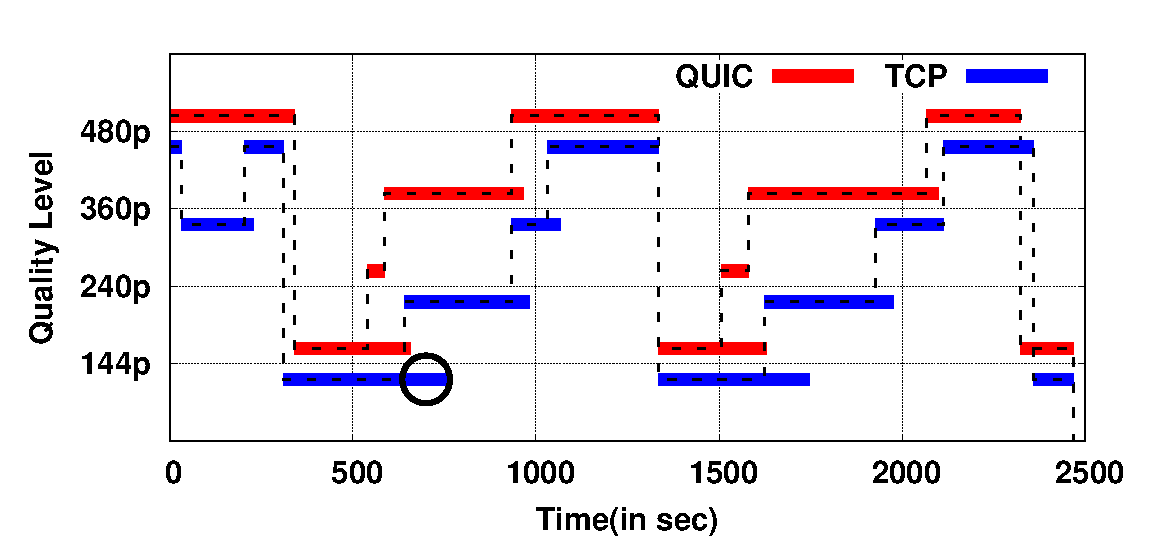
\includegraphics[width=0.7\linewidth]{img/plotdata/video/plot_timerange}
\caption{Segments downloaded at different quality levels for a YouTube video with ID $<$OJZgOOOE1zY$>$}
\label{fig:plot_timerange}
\end{figure}

Here we consider the data from a sample video with YouTube video ID $<$OJZgOOOE1zY$>$  (last accessed on 17th May, 2017) among the videos that we have downloaded during the data collection phase. \fig\ref{fig:plot_timerange} shows the downloaded segments at different video quality for this video with respect to time. 
%We plot the quality switching distribution for both the cases -- when the video was streamed through QUIC (the red line) and when the video was streamed through TCP (the blue line). 
Here we can see that there is a slight overlap between the downloaded segments of two qualities, when the streaming client upgrades the video quality from one to another. During quality upgrade, YouTube streaming client takes an restrictive approach by downloading the video segments of two different qualities simultaneously for some amount of time, so that it can revert back to the low quality immediately in case of request failure for the high quality video segment. %, in case the download request for the high quality video segment is successful. 
However, this results in data waste when the request for high quality video segment is indeed successful. 
%Next we analyze the impact of QUIC and TCP over this data wastage during adaptive streaming over the web.   

\subsubsection{Data Waste Due to Adaptive Streaming: QUIC vs TCP}
%\clearpage
%\begin{figure}[ht!]
%    \centering
%    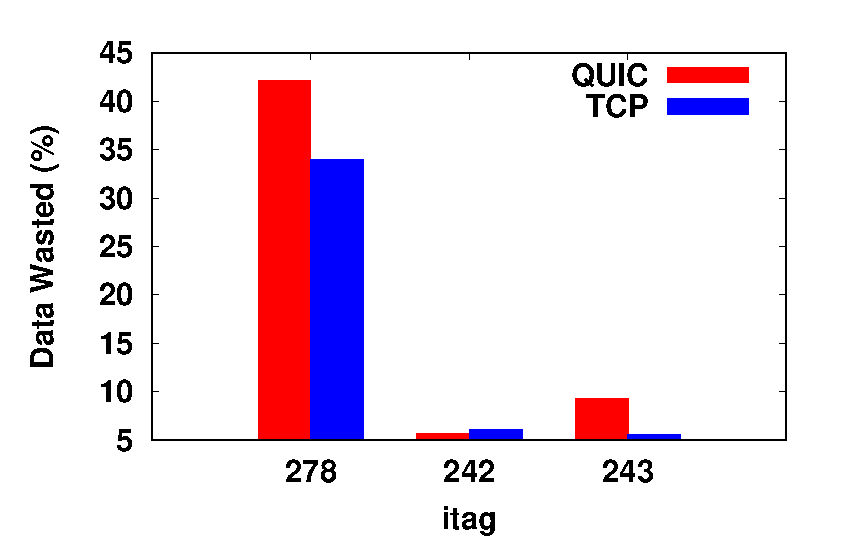
\includegraphics[width=0.9\linewidth]{img/CDF/Data_wasted_percent}
%    \caption{Amount of Data Wasted \notesc{Plot the percentage as given in the table -- then this figure is not required}\noteam{Done}}
%    \label{fig:rabuf76q1}
%\end{figure}

\begin{figure}[!t]
	\captionsetup[subfigure]{}
	\begin{center}
%		\subfloat[\label{fig:wasted_quality} At Different Quality]{
%			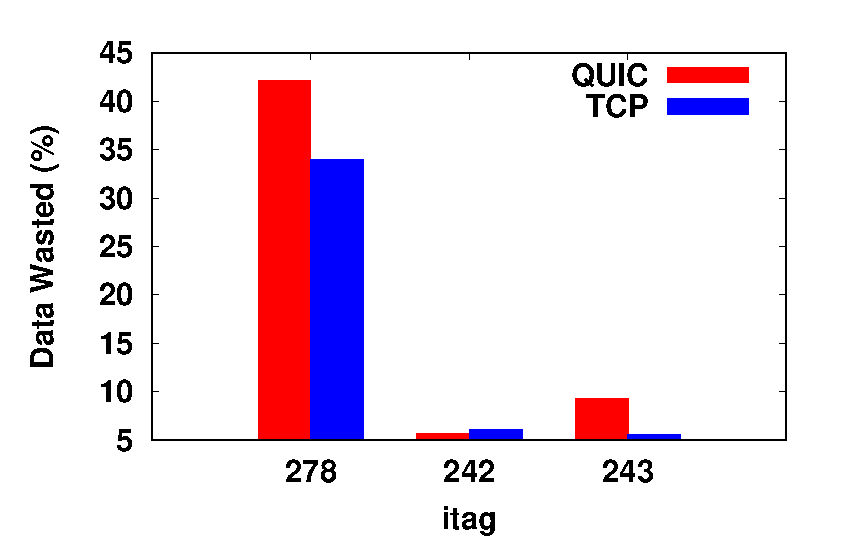
\includegraphics[width=0.48\linewidth]{img/CDF/Data_wasted_percent}
%		}
%		\subfloat[\label{fig:wasted_band}At Different Bandwidth]{
%			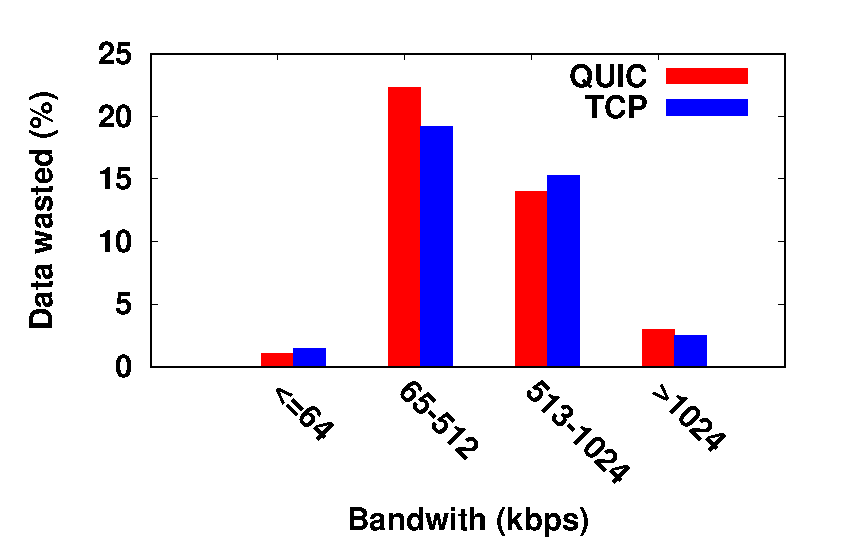
\includegraphics[width=0.48\linewidth]{img/CDF/data_wasted_bw}
%		}
        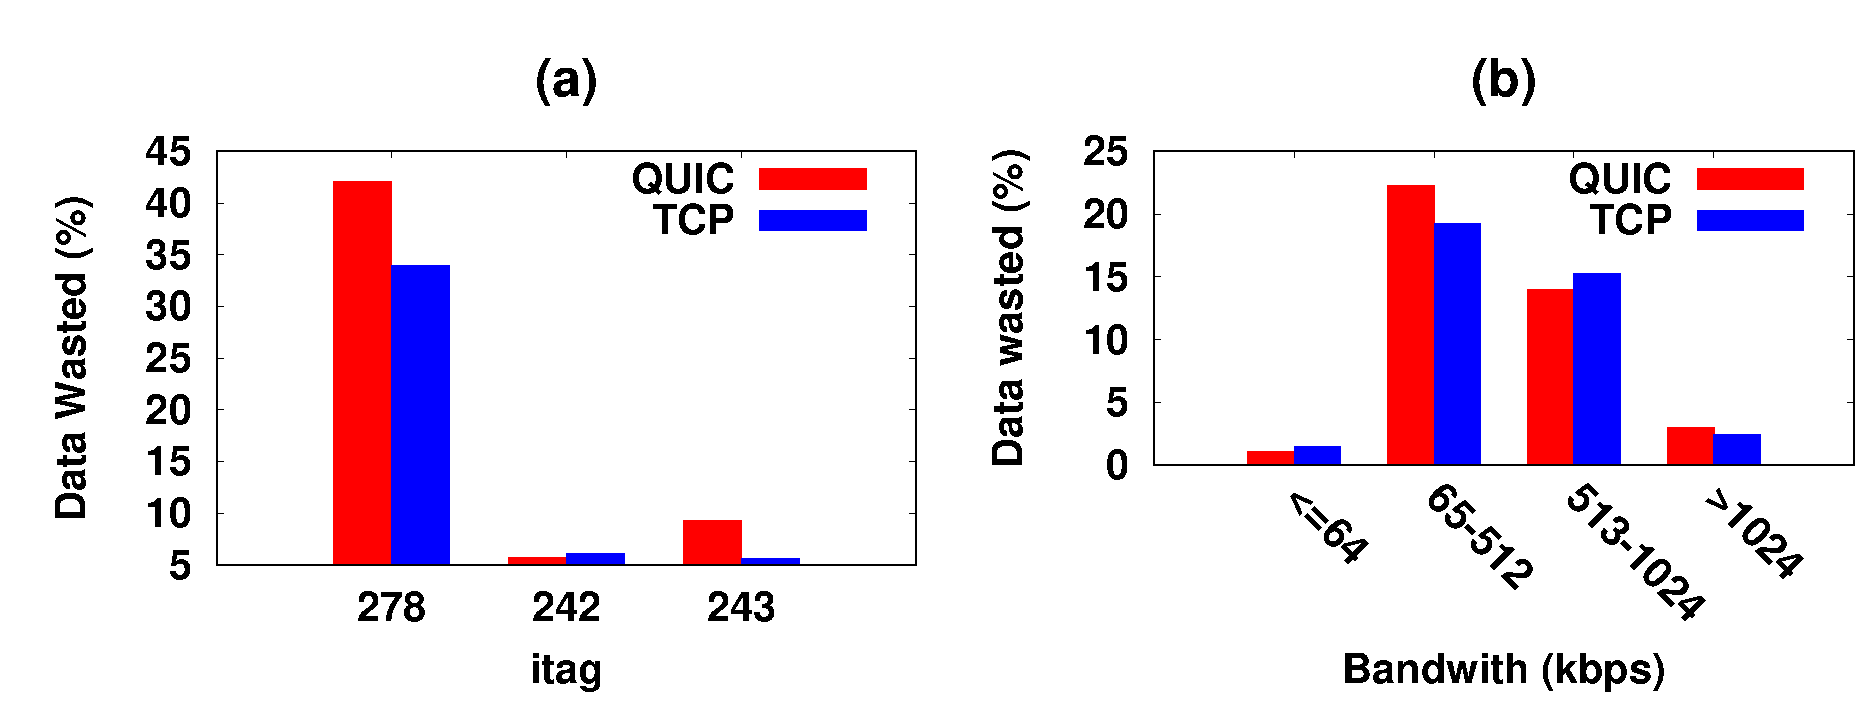
\includegraphics[width=0.9\linewidth]{img/plotdata/CDF/downloaded/data_wasted_itag_bw}
		\caption{\label{fig:data_wasted}Data wasted: (a) Different quality levels, (b) Different channel bandwidth}
	\end{center}
\end{figure}


%\notesc{Percentage of data wasted at various bandwidth buckets -- (a) $\leq 64$ Kbps, (b) $65-512$ Kbps, (c) $513-1024$ Kbps, (d) $> 1024$ Kbps}

%
%\begin{table}[ht!]
%    \centering
%    \small
%    \begin{tabular}{||c |c |c|c|c||} 
%        \hline
%        \textbf{Itag} & \textbf{Resolution} & \textbf{Downloaded}& \textbf{Wasted}& \textbf{\%}  \\ 
%        & & \textbf{(Mb)}& \textbf{(Mb)}& \textbf{Wasted}\\ 
%        \hline\hline
%        278 & 256x144 & 7669 & 3230 & 42.12\%\\ 
%        \hline
%        242 & 426x240 & 21232 & 1219 &5.74\%\\ 
%        \hline
%        243 & 640x360 & 44894 & 4187 &9.33\%\\ 
%        \hline
%        \hline
%        Total &  & 73795 & 8636 &11.7\%\\ 
%        \hline
%    \end{tabular}
%    \caption{Data Wastage for QUIC}
%    \label{table:3}
%\end{table}

%\begin{table}[ht!]
%    \centering
%%    \scriptsize
%    \small
%    \begin{tabular}{||c |c |c|c|c||} 
%        \hline
%        \textbf{Itag} & \textbf{Resolution} & \textbf{Downloaded}& \textbf{Wasted}& \textbf{\%}  \\
%        & & \textbf{(Mb)}& \textbf{(Mb)}& \textbf{Wasted }  \\
%        \hline\hline
%        278 & 256x144 & 10049 & 3412 & 33.95\%\\ 
%        \hline
%        242 & 426x240 & 23028 & 1399 &6.07\%\\ 
%        \hline
%        243 & 640x360 & 37911 & 2134 &5.63\%\\ 
%        \hline
%        \hline
%        Total &  & 70988 & 6945 &9.78\%\\ 
%        \hline
%    \end{tabular}
%    \caption{Data Wastage for TCP}
%    \label{table:4}
%\end{table}
\begin{figure*}[!t]
	\captionsetup[subfigure]{}
	\begin{center}
		%		\subfloat[\label{fig:plot_itag_pdf_bucket1}Bandwidth $\leq 64$ Kbps]{
		%			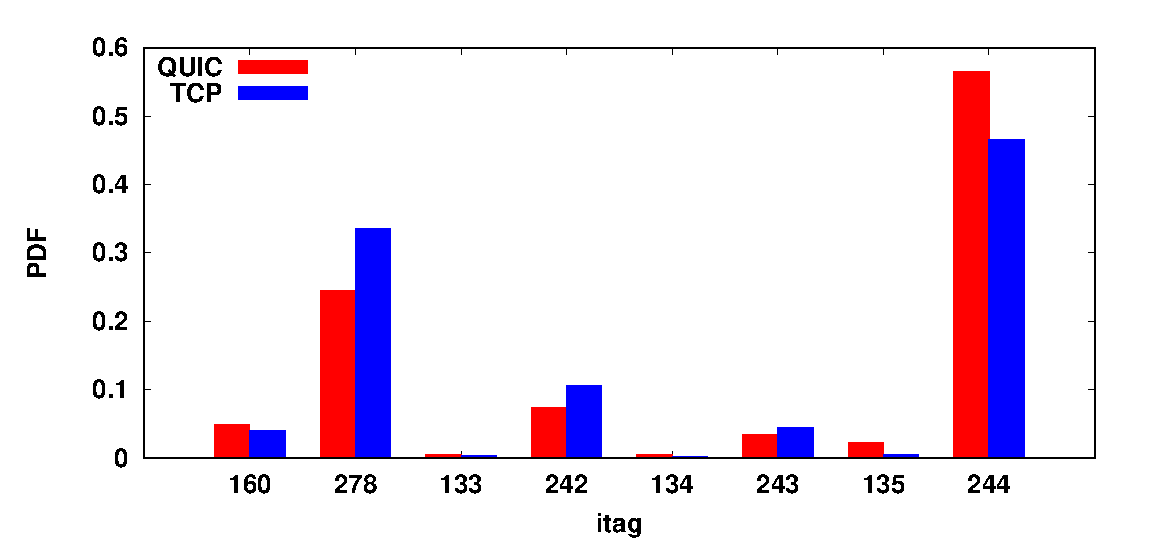
\includegraphics[width=0.32\linewidth]{img/PDF/plot_itag_pdf_bucket1}
		%		}
		%		\subfloat[\label{fig:plot_itag_pdf_bucket2} $64$ Kbps $<$ Bandwidth $ \leq 1024$ Kbps]{
		%			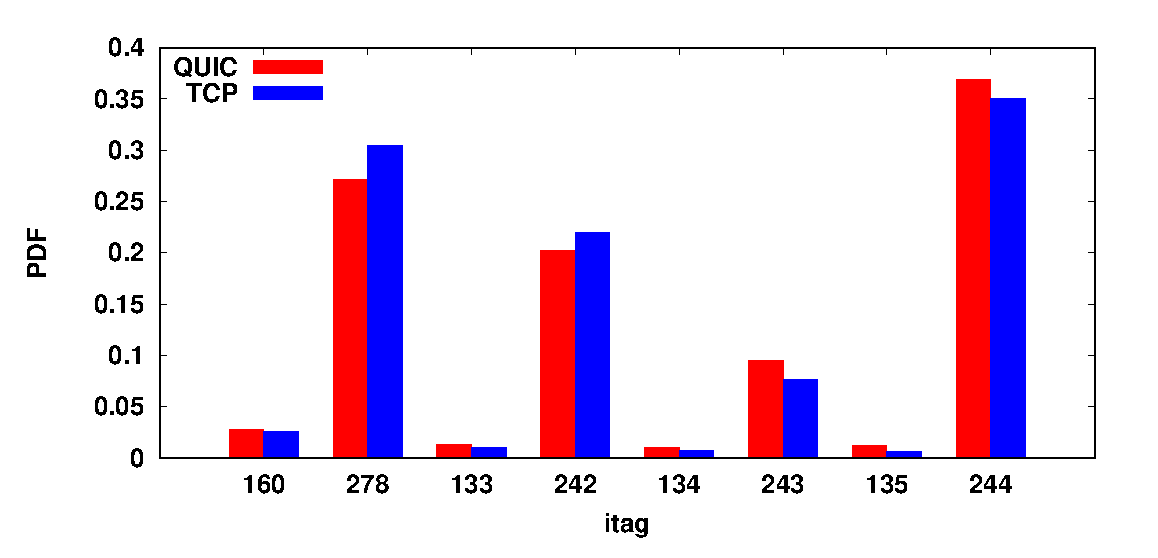
\includegraphics[width=0.32\linewidth]{img/PDF/plot_itag_pdf_bucket2}
		%		}
		%		\subfloat[\label{fig:plot_itag_pdf_bucket3}Bandwidth  $> 1024$ Kbps]{
		%			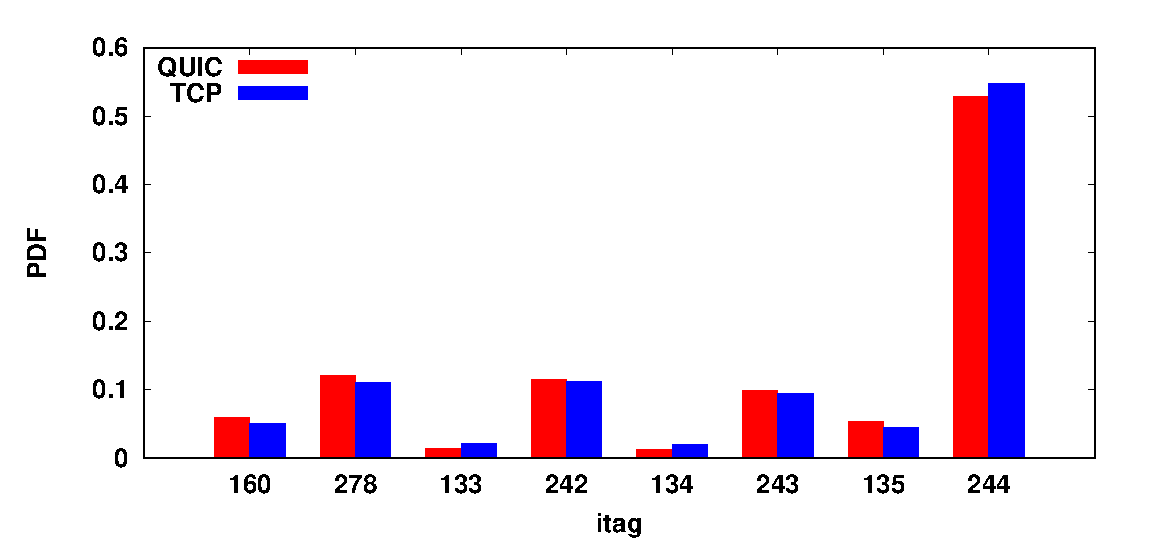
\includegraphics[width=0.32\linewidth]{img/PDF/plot_itag_pdf_bucket3}
		%		}
		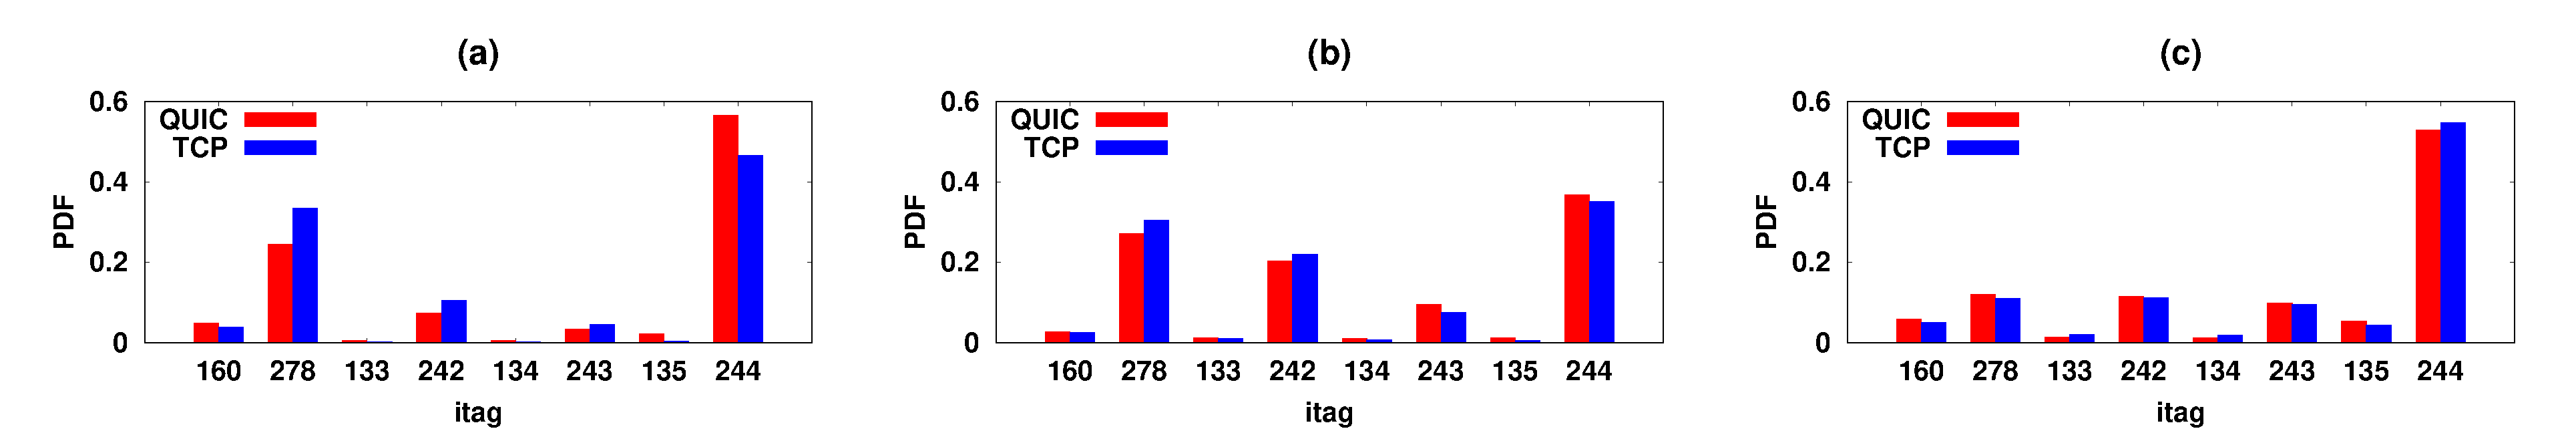
\includegraphics[width=0.8\linewidth]{img/plotdata/PDF/itag/plot_itag_pdf_bucket123}
		\caption{\label{fig:quality_change}Change for quality levels at different bandwidth: (a) $\leq 64$ Kbps, (b)  between $64$ and $1024$ Kbps, (c) $> 1024$ Kbps}
	\end{center}
\end{figure*}

\fig\ref{fig:data_wasted} compares \ac{QUIC} enabled streaming and \ac{TCP} enabled streaming in terms of percentage of data waste during quality upgrades. 
%Here we show the percentage data waste (percentage of total downloaded data that has not been played during the video rendering) for different quality levels, when the YouTube client switches the quality from this level to a higher level. 
We observe that data waste with \ac{QUIC} is more compared to \ac{TCP}. Further, data waste is comparatively high when the available bandwidth is less that $512$ Kbps (\fig\ref{fig:data_wasted}(b)). 
%It can be noted that frequent quality switching increases the amount of data wastage. 
By observing data logs, we have found that for \ac{QUIC} enabled streaming, the YouTube client tries to make more number of quality upgrade attempts at the low bandwidth, which are not successful. 
%In the next subsection, we give a detailed analysis of this behavior. 
Consequently, \ac{QUIC} results in more data waste. In the next section, we give a detailed view of this. 
%\fig\ref{fig:wasted_band} plots the percentage data wasted for different network conditions measured in terms of available channel bandwidth. We observe that 
%Further, 
%This supports our hypothesis that the quality upgrade attempts at low bandwidth under QUIC is not stable that results in comparatively high data wastage. In the next section, we discuss additional results in support of this hypothesis and to analyze the video streaming behavior of QUIC and TCP under different channel conditions. 


%\subsection{Comparison of Streaming data rate between QUIC and TCP}
%In this section we will examine whether the streaming data rate variation  whenever the bandwidth changes, is similar in QUIC and TCP. To compare the behavior of streaming data rate adaptation, we plot how the requested video segment length (specified by the \textit{range} parameter) per video playback request, changes with change in link bandwidth in \fig\ref{fig:rser1}. For this, we convert the byte range mentioned in the video playback request to the equivalent video playback time, and find out the video segment length in terms of playback time. Whenever the link bandwidth increases, YouTube first increases the segment length of lower quality video and buffers maximum amount of video data. It then switches to the higher quality video but with smaller segment lengths. At this point, we observe an overlap between the segments of two different video qualities. It then progressively increases the segment length and repeats the procedure for the next higher quality level video if the link quality improves further (measured through the increase rate of \textit{rbuf}). However, when the link quality drops, in a similar way, YouTube first starts requesting for same quality video chunks of smaller segments, and drops the segment length. If it still observes a drop in \textit{rbuf} after reducing the segment length in the playback requests, then it switches to request for the next lower quality level video chunks of smaller segments. If the \textit{rbuf} becomes stable, then only it again increases the segment length. This behaviour is similar to both QUIC and TCP over YouTube but from the plots we can observe that QUIC is able to switch to higher quality from a lower quality in a shorter interval of time when compared to TCP. 
%
%
%%\newpage
%%\begin{figure}[!ht] 
%%    \centering
%%    \begin{minipage}{0.45\linewidth}
%%        \includegraphics[width=\linewidth]{img/QUICPlots/plot_sengmentLength} 
%%        \caption{QUIC}
%%        \label{fig:seg1Q}
%%    \end{minipage}
%%    \begin{minipage}{0.45\linewidth}
%%        \includegraphics[width=\linewidth]{img/TCPPlots/plot_sengmentLength}
%%        \caption{TCP}
%%        \label{fig:rseg1T}
%%    \end{minipage} 
%%    \caption{Plot for \textit{Segment Length} over time for a YouTube video of id $<$OJZgOOOE1zY$>$}
%%    \label{fig:rser1}
%%\end{figure}
%\begin{figure}[!t]
%    \captionsetup[subfigure]{}
%    \begin{center}
%        \subfloat[\label{fig:seg1Q}QUIC]{
%            \includegraphics[width=0.48\linewidth]{img/QUICPlots/plot_sengmentLength}
%        }
%        \subfloat[\label{fig:rseg1T}TCP]{
%            \includegraphics[width=0.48\linewidth]{img/TCPPlots/plot_sengmentLength}
%        }
%        
%        \caption{\label{fig:rser1}Plot for \textit{Segment Length} over time for a YouTube video of id $<$OJZgOOOE1zY$>$}
%    \end{center}
%\end{figure}
%%\clearpage
%
%%\section{Comparison of Video Quality observed over time between QUIC and TCP}
%From \fig\ref{fig:rser1}, we observe that as link quality increases, \textit{rbuf} also increases, and YouTube client progressively makes requests for higher \textit{itag} values. Further, whenever the value of \textit{rbuf} drops, YouTube client switches \textit{itag} requests for a lower video quality. We already know that YouTube video quality adaptation algorithm is based on the client’s observation of the change in receive buffer – a sharp increase in received buffer gives an indication for fetching data of higher video quality, whereas YouTube takes a conservative approach of requesting data for lower video quality whenever the client observes a sharp drop in receive buffer size.
%
%From the earlier discussion, we know that \textit{range} parameter gives the byte range of the video streaming data for which the client sent a request to the server. We first convert this range parameter to equivalent video segment length in terms of video playback time. This can be done by looking into the video file header that provides a mapping between the byte range and playback time. We use the Python package {\fontfamily{qcr}\selectfont python-ebml} to extract such information from the video files. The figures in \fig\ref{fig:rserr1} plots the video segments (in terms of video playback time, as shown in Xaxis) and the corresponding \textit{itag} values for which the client makes a request. YouTube takes an opportunistic approach for downloading higher quality video segments when the link quality improves, but takes a conservative approach when the link quality drops. In the opportunistic approach, it downloads the video chunks of both the video qualities in parallel, whenever it decides to switch from the lower quality to the higher quality. However, in the conservative approach, it directly sends the request for lower quality video when the link quality drops. That is why we notice an an overlap between the segments of lower quality and higher quality when the video quality improves.
%
%When we observe the plot for a single video (\fig\ref{fig:rser1} and \fig\ref{fig:rserr1}), we can see that there are overlaps between the segment downloaded. So, there is some data wastage is happening. In next section, we compare data wastages during video playback using the normal TCP and the QUIC.
%
%%When we observe the plot for a single video (\fig\ref{fig:rserr1}), it is evident that QUIC is able to maintain video quality that is higher or same as that of TCP in most cases. From these three plots (\noteam{I could not figure out which three.}) we can expect that DASH will perform better when QUIC is employed as transport layer protocol rather than TCP in terms of video quality. In order to prove the above hypothesis we will show the Cumulative Distribute Function graphs collected over 175 videos in the next section.
%
%%\begin{figure}[!ht] 
%%    \centering
%%    \begin{minipage}{0.45\linewidth}
%%        \includegraphics[width=\linewidth]{img/QUICPlots/plot_timerange} 
%%        \caption{QUIC}
%%        \label{fig:rseg1Q}
%%    \end{minipage}
%%    \begin{minipage}{0.45\linewidth}
%%        \includegraphics[width=\linewidth]{img/TCPPlots/plot_timerange}
%%        \caption{TCP}
%%        \label{fig:rsegr1T}
%%    \end{minipage} 
%%    \caption{Plot for time range of different qualities for a YouTube video of id $<$OJZgOOOE1zY$>$}
%%    \label{fig:rserr1}
%%\end{figure}
%
%\begin{figure}[!t]
%    \captionsetup[subfigure]{}
%    \begin{center}
%        \subfloat[\label{fig:rseg1Q}QUIC]{
%            \includegraphics[width=0.48\linewidth]{img/QUICPlots/plot_timerange}
%        }
%        \subfloat[\label{fig:rsegr1T}TCP]{
%            \includegraphics[width=0.48\linewidth]{img/TCPPlots/plot_timerange}
%        }
%        
%        \caption{\label{fig:rserr1}Plot for \textit{Time Range} over time for a YouTube video of id $<$OJZgOOOE1zY$>$}
%    \end{center}
%\end{figure}
%%\clearpage


\subsection{Impact of Channel Bandwidth over Video Streaming: QUIC vs TCP}
From the previous discussion and analysis, we have observed that the performance of video streaming over \ac{QUIC} has a dependency over the available channel bandwidth. 
%The data wastage due to YouTube adaptive streaming is more when channel bandwidth is low. To explore this behavior further, we next analyze the adaptive streaming behavior over QUIC under different channel conditions measured in terms of available channel bandwidth. 
Here, we particularly look the evolution of three parameters at different available bandwidth, which control the adaptive streaming behavior -- (a) quality switching (using \textit{itag}), (b) buffer occupancy at the YouTube streaming client (using \textit{rbuf}) and (c) segment length adaptation during streaming (using \textit{range} ). We consider three channel conditions -- (a) poor (available bandwidth is less than $64$ Kbps), (b) medium (available bandwidth is in between $64$ Kbps and $1$ Mbps), and (c) good (available bandwidth is more than $1$ Mbps).

\subsubsection{Video Quality Adaptation}
%For a particular bandwidth level we counted the number of requests made for each \textit{itag} and from that we calculated the probability for an  \textit{itag} as the number of requests made for that itag divided by total number of requests made.
%
%\begin{figure}[!ht]
%    \centering
%    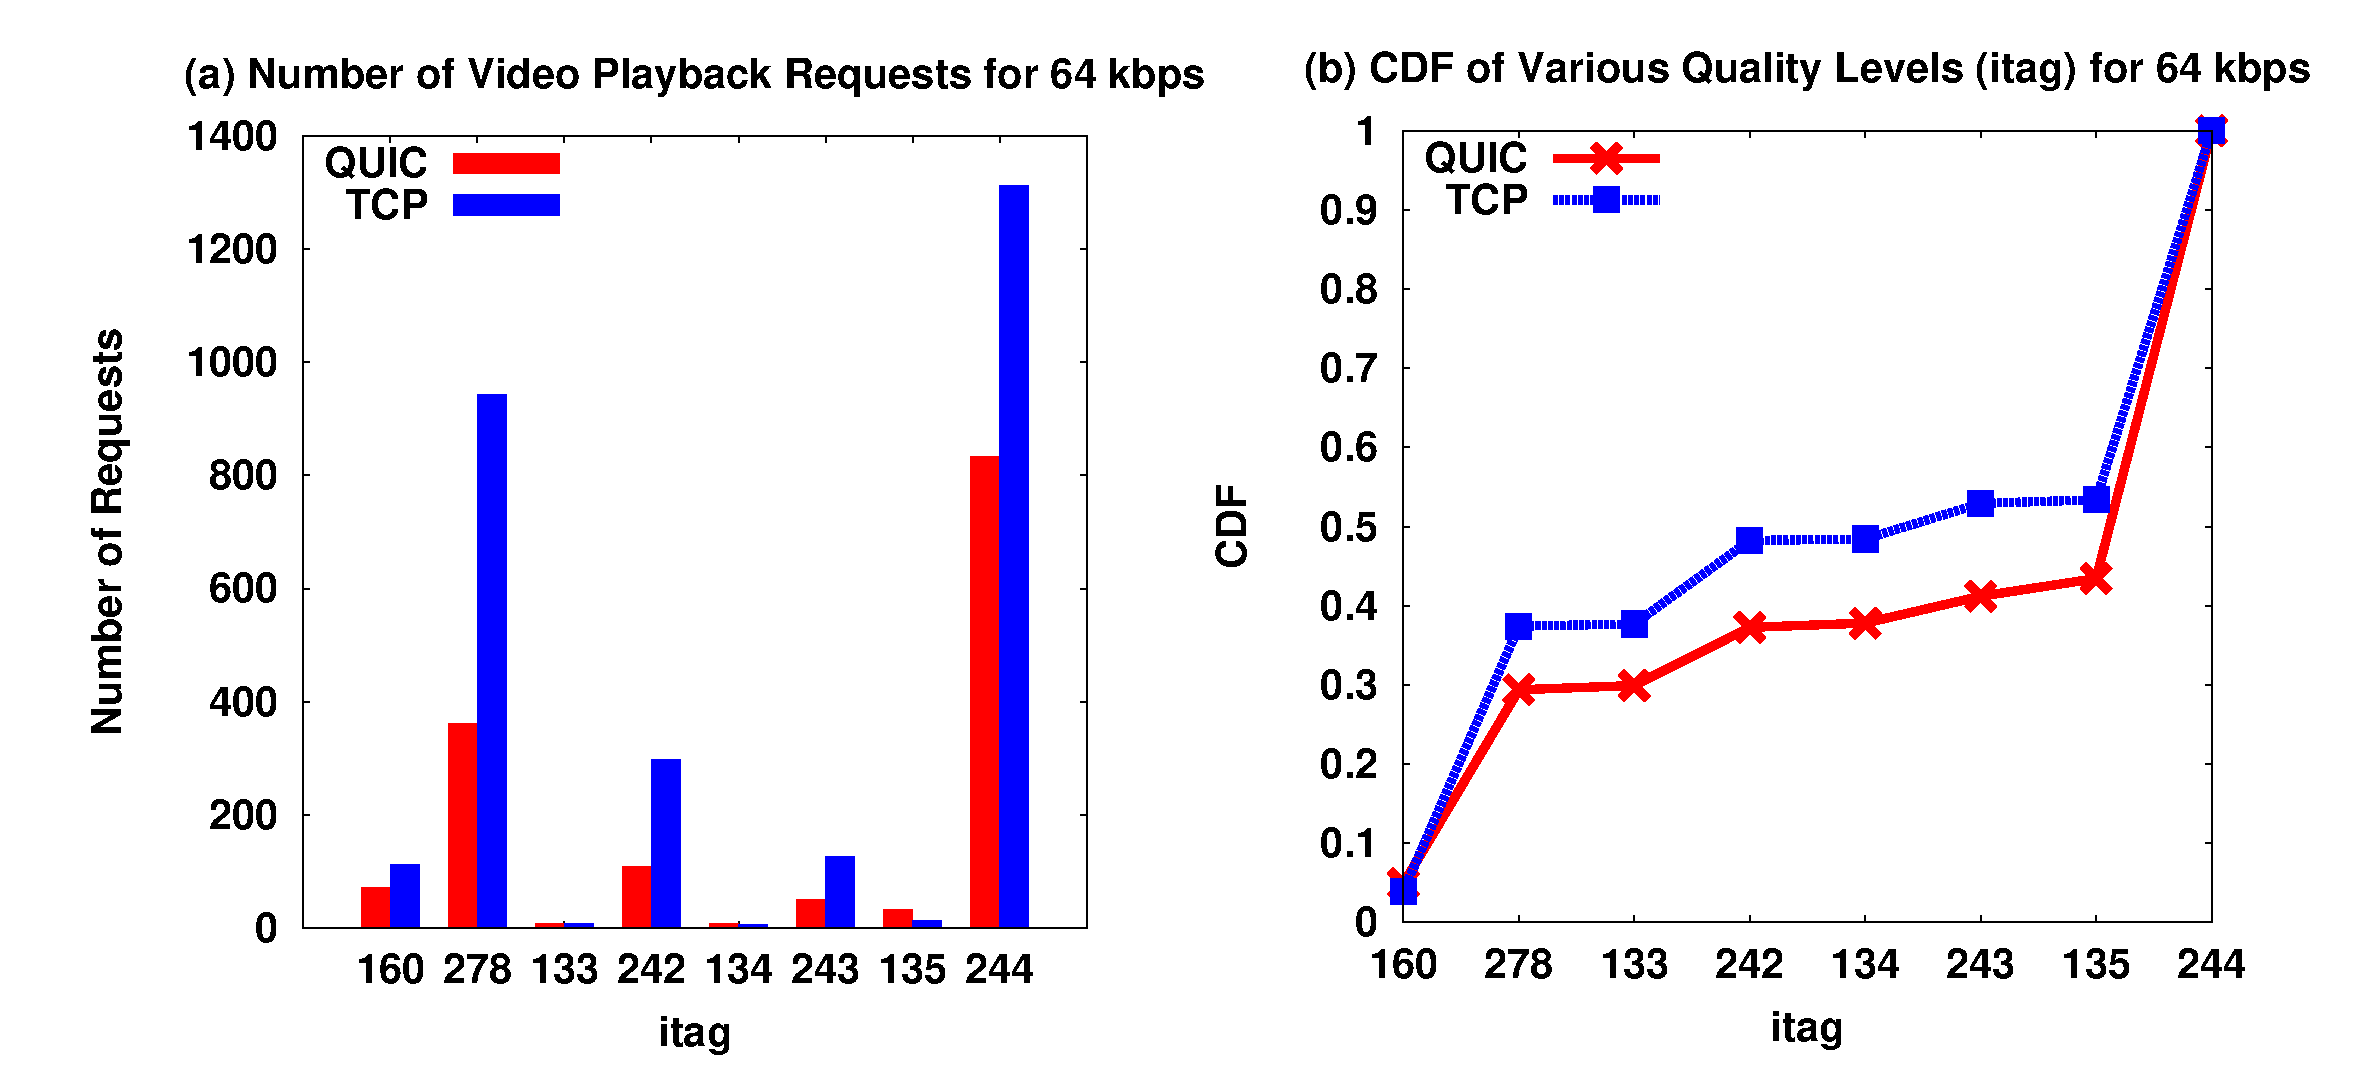
\includegraphics[width=\linewidth]{img/CDF/plot_itag_65536}
%    \caption{Number of requests and CDF of itag at 64 kbps}
%    \label{fig:itag6556}
%\end{figure}
%
%\begin{figure}[!ht]
%    \centering
%    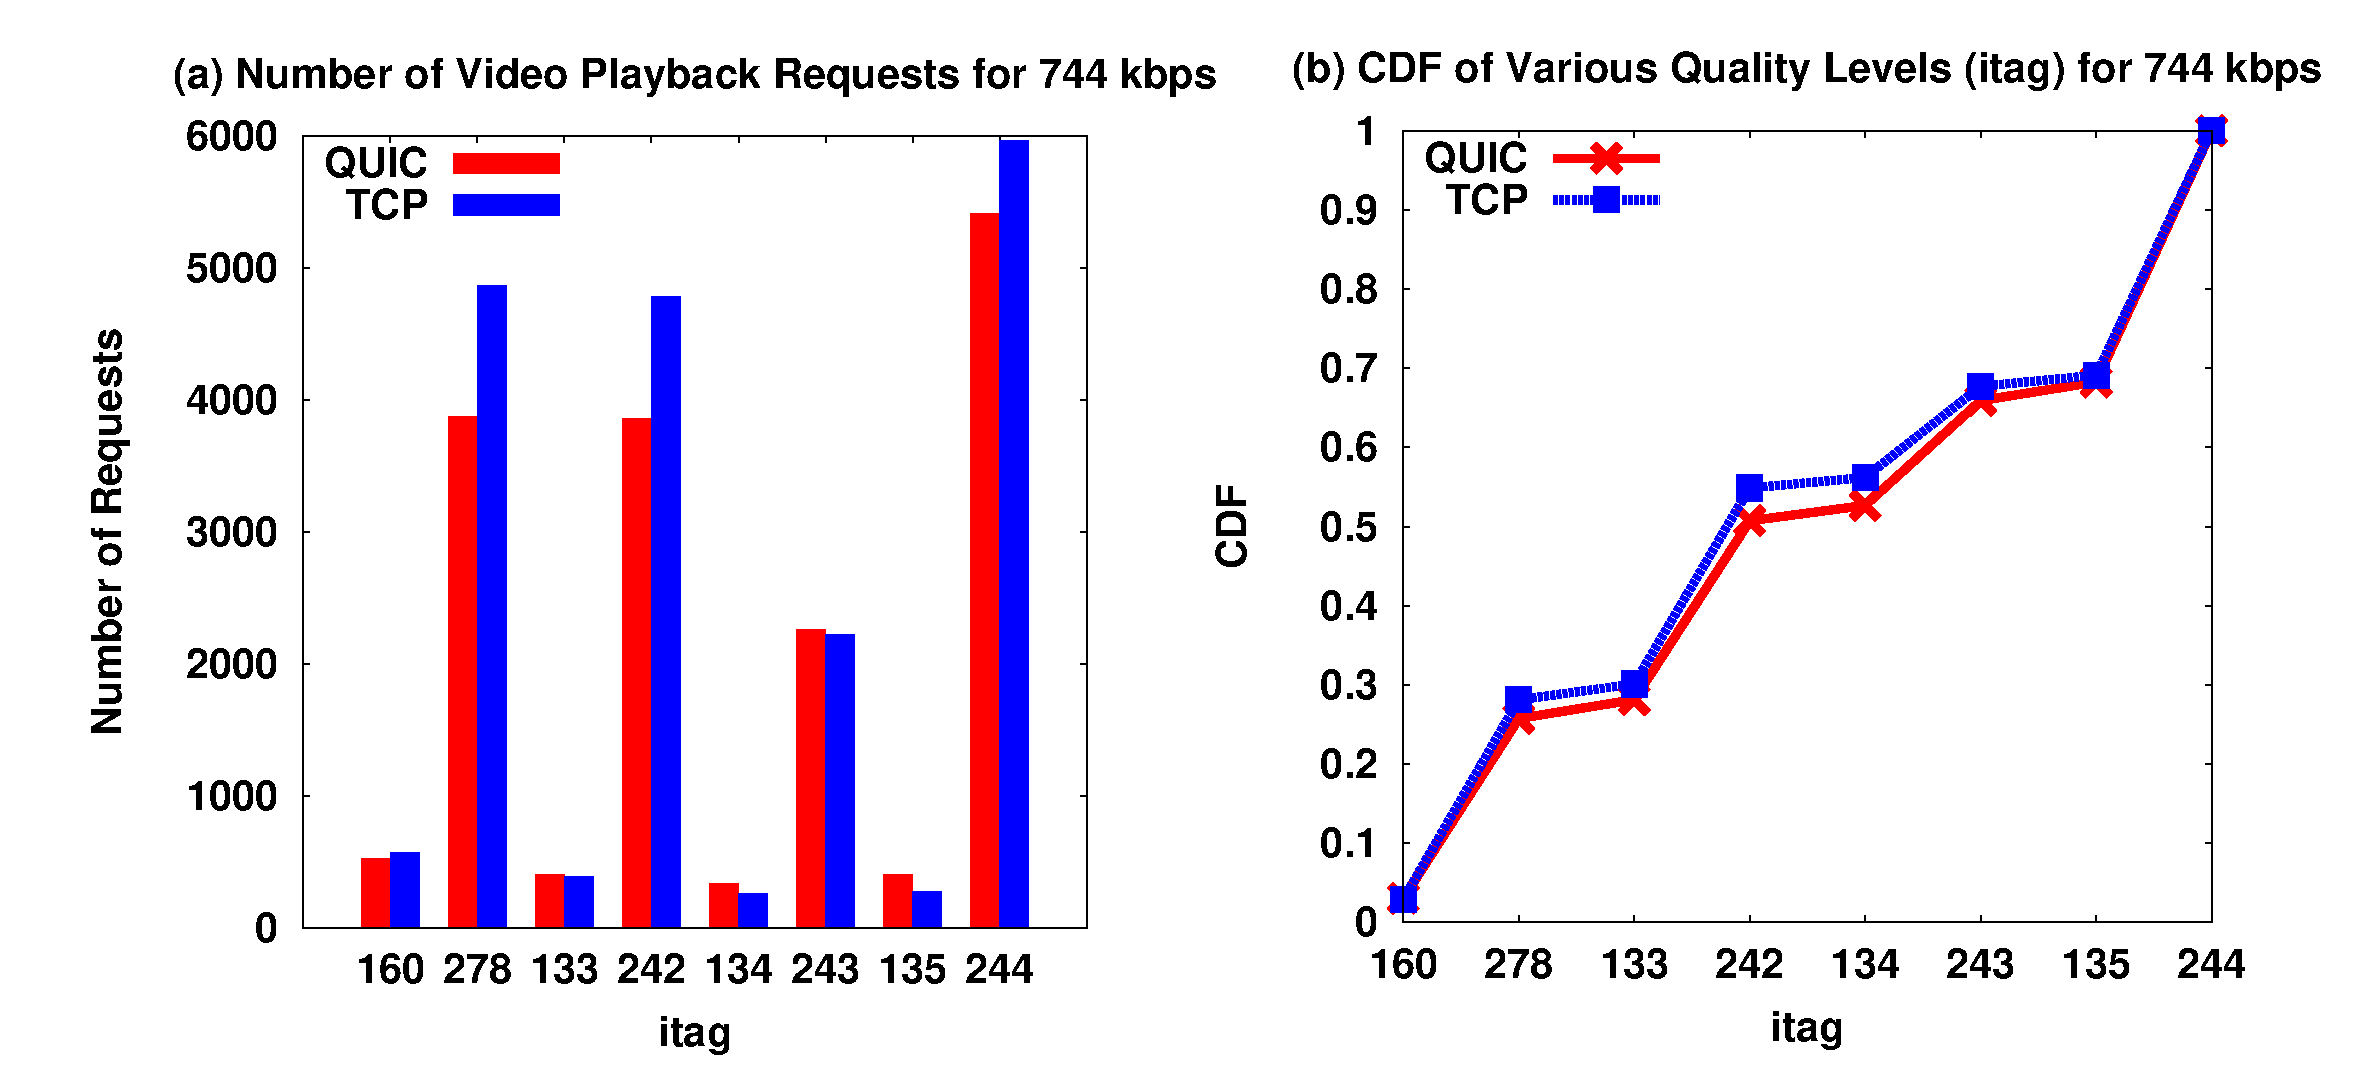
\includegraphics[width=\linewidth]{img/CDF/plot_itag_761856}
%    \caption{Number of requests and CDF of itag at 744 kbps}
%    \label{fig:itag761}
%\end{figure}
%
%
%
%\begin{figure}[h]
%    \centering
%    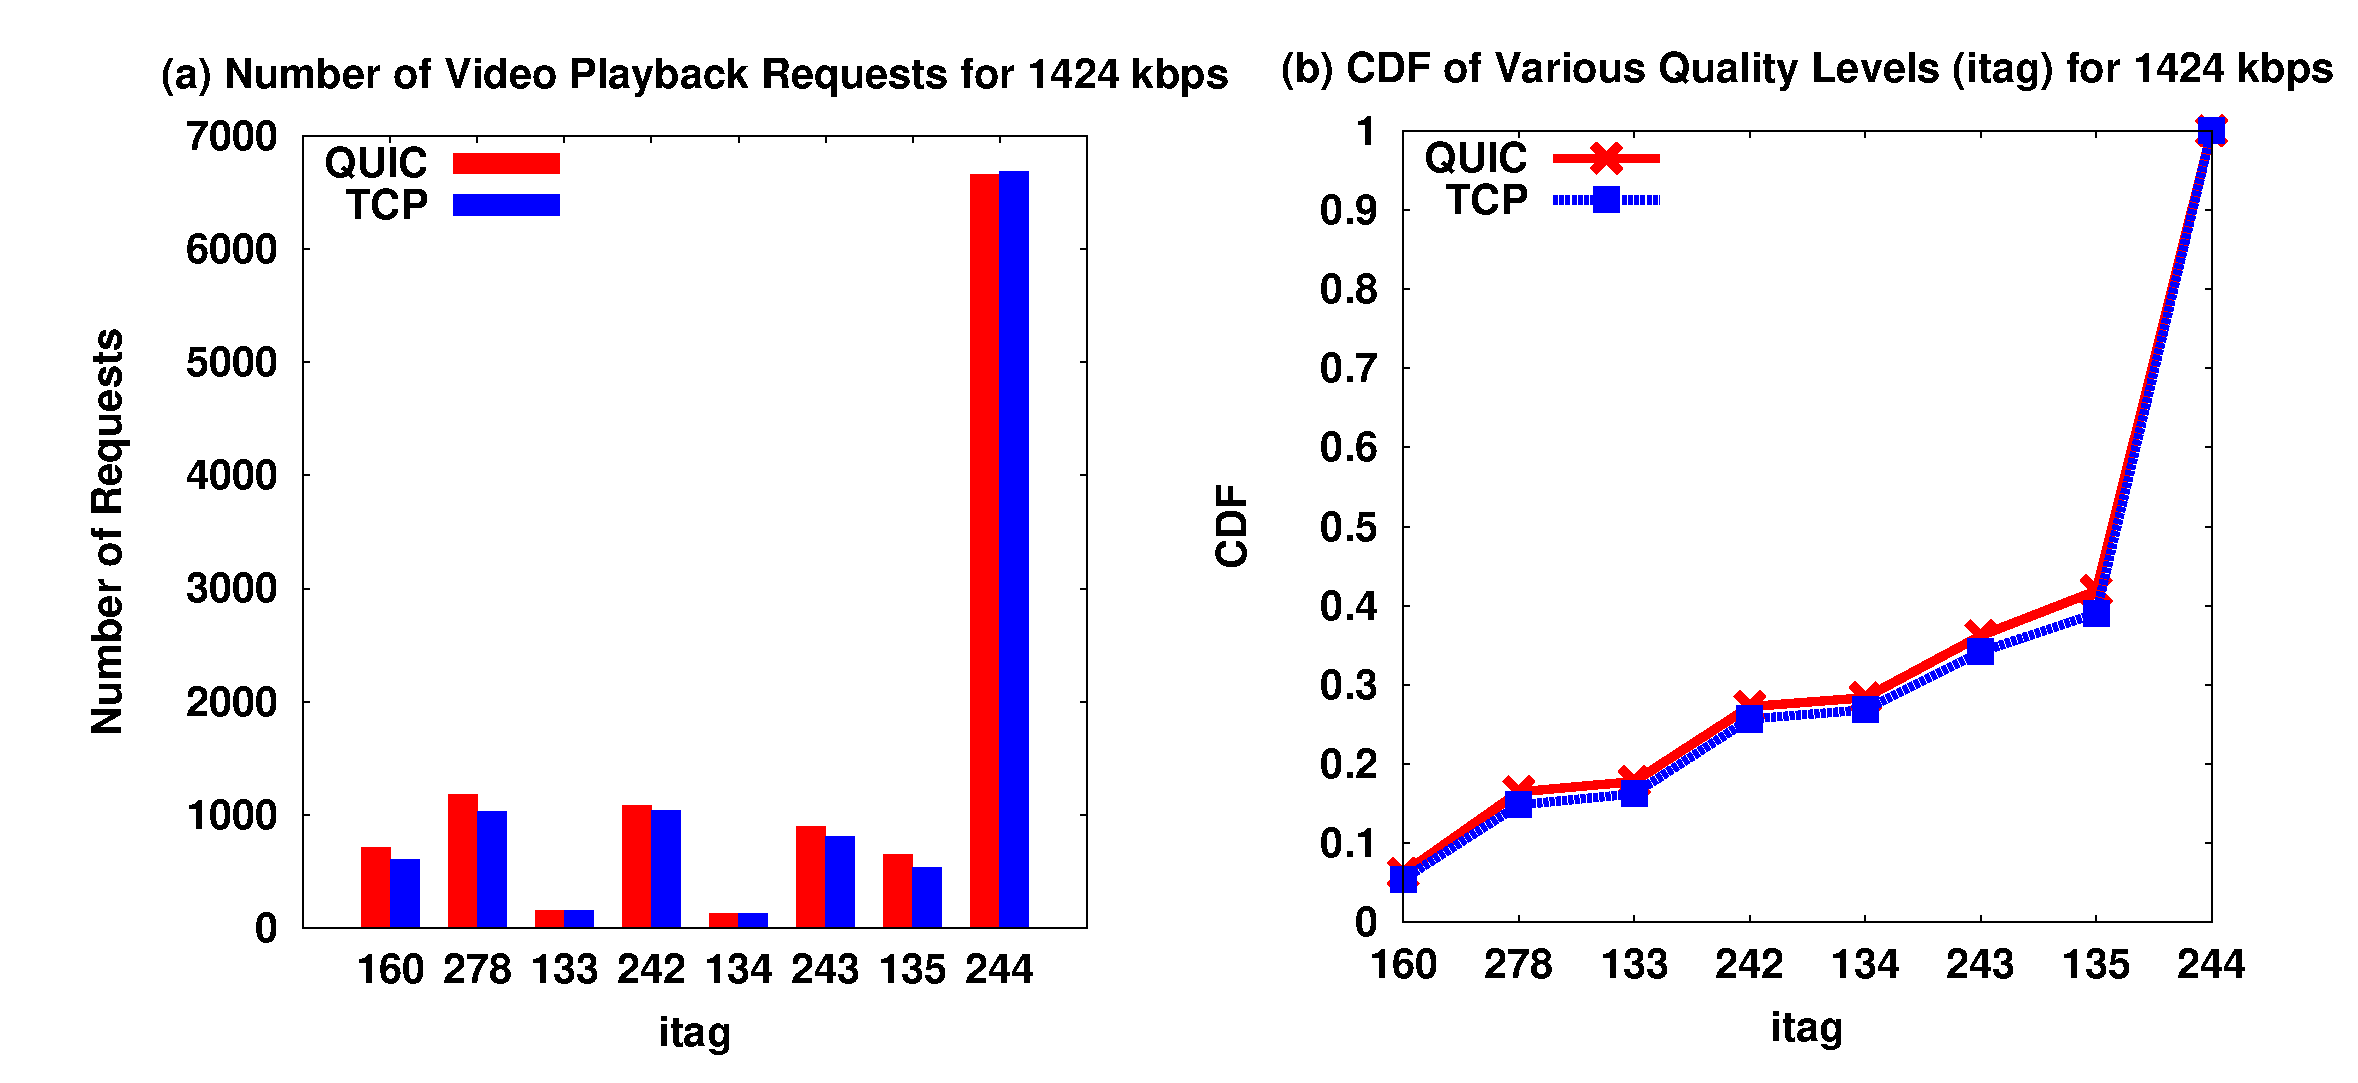
\includegraphics[width=\linewidth]{img/CDF/plot_itag_1458176}
%    \caption{Number of requests and CDF of itag at 1424 kbps}
%    \label{fig:itag76111}
%\end{figure}




We compute the \ac{PDF} for various \textit{itag} values during the video bitrate adaption procedure, as shown in \fig\ref{fig:quality_change}. 
%\begin{addmargin}[2.1cm]{2.1cm}
We observe that at poor bandwidth, \ac{QUIC} has higher tendency than \ac{TCP} towards high quality videos, but as the bandwidth increases, both \ac{QUIC} and \ac{TCP} show similar tendencies towards video quality adaptation. So, \ac{QUIC} may improve the viewing performance with a better video quality than \ac{TCP}  at poor channel connection. However, as we observed, many of these quality upgrades are not very stable, and this frequent quality upgrades result in more data waste, as we observed earlier. 
%At lower speeds QUIC does not make as many requests to the server as TCP makes but at higher speeds both the protocols makes the same number of requests. This implies that QUIC is more aware of the network conditions than TCP. In the above plots when the bandwidth is at 64Kbps TCP has made almost twice the number of requests as QUIC made. This is because at 64Kbps when almost all the packets are dropped, TCP unable to quickly recognize the change in bandwidth makes the request for the same higher itag value and when they fail it makes requests for lower itags. For the total set of 175 videos the number of requests made by QUIC are lesser in number when compared to TCP which implies that QUIC requires less number of requests to serve the same or higher quality data.
%\end{addmargin}
%\restoregeometry

\subsubsection{Buffering at the Playback Client}

\begin{figure}[!t]
	\captionsetup[subfigure]{}
	\begin{center}
%		\subfloat[\label{fig:rbuf_bucket1}Bandwidth $ \leq 64 $ Kbps]{
%			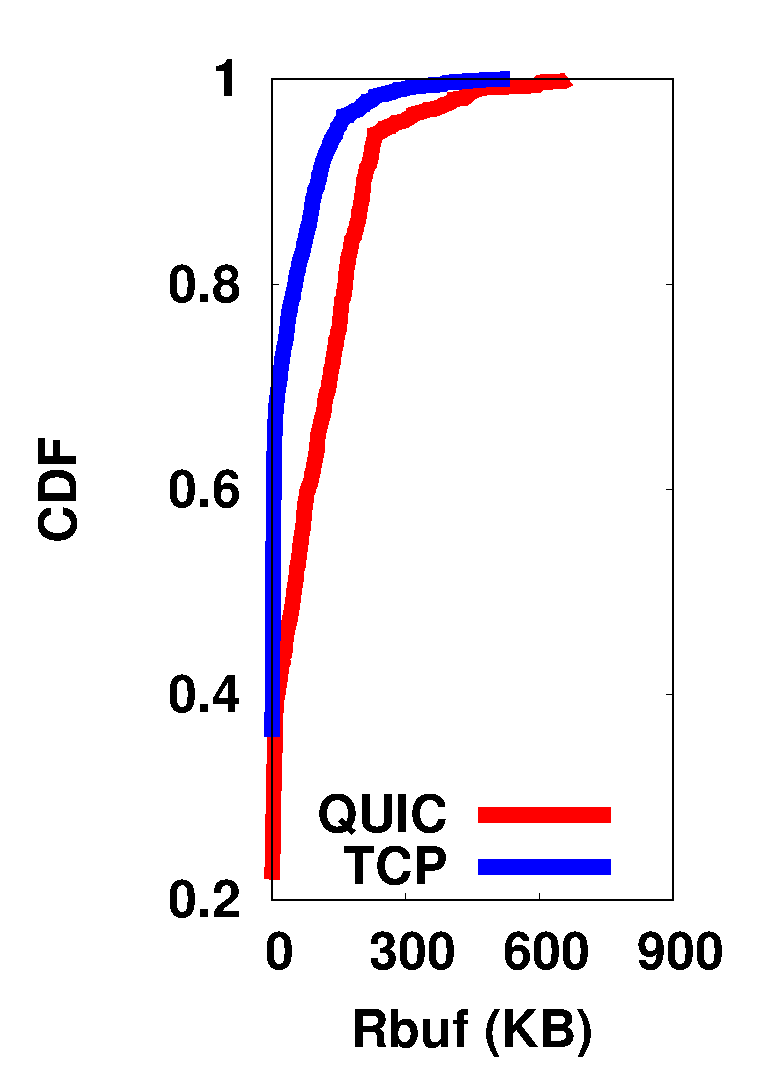
\includegraphics[width=0.32\linewidth]{img/CDF/plot_rbuf_bucket1}
%		}
%		\subfloat[\label{fig:rbuf_bucket2} $64$ Kbps $<$ Bandwidth $ \leq 1024$ Kbps]{
%			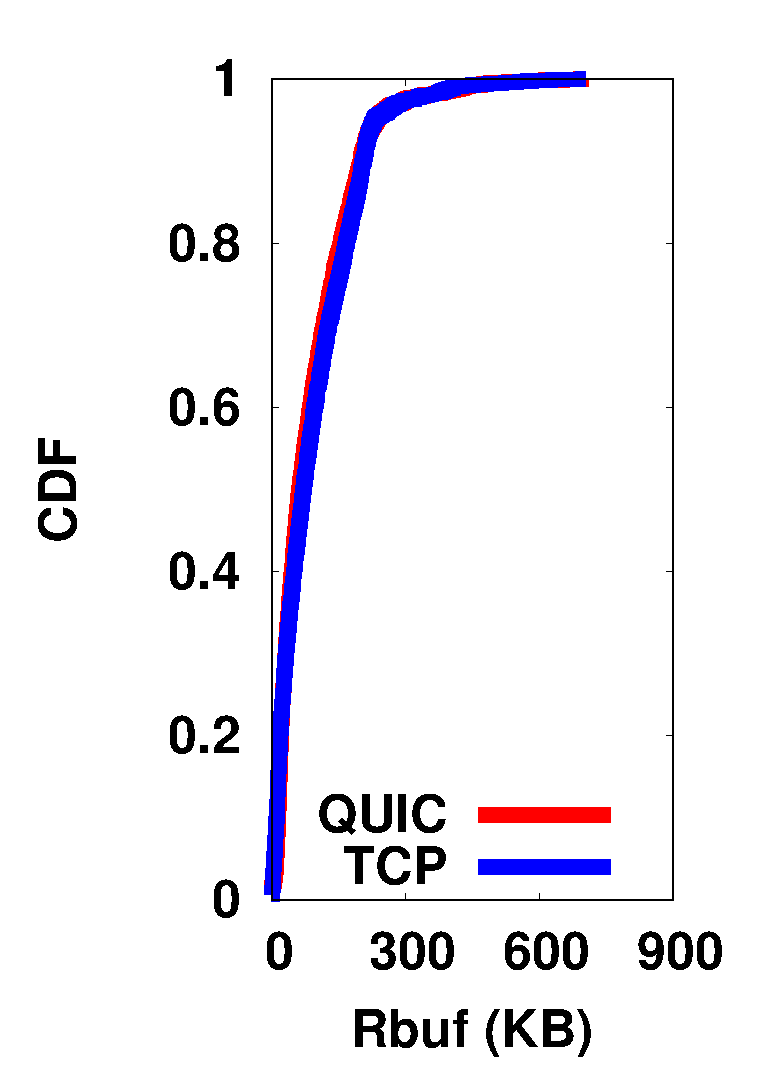
\includegraphics[width=0.32\linewidth]{img/CDF/plot_rbuf_bucket2}
%		}
%		\subfloat[\label{fig:rbuf_bucket3}Bandwidth  $> 1024$ Kbps]{
%			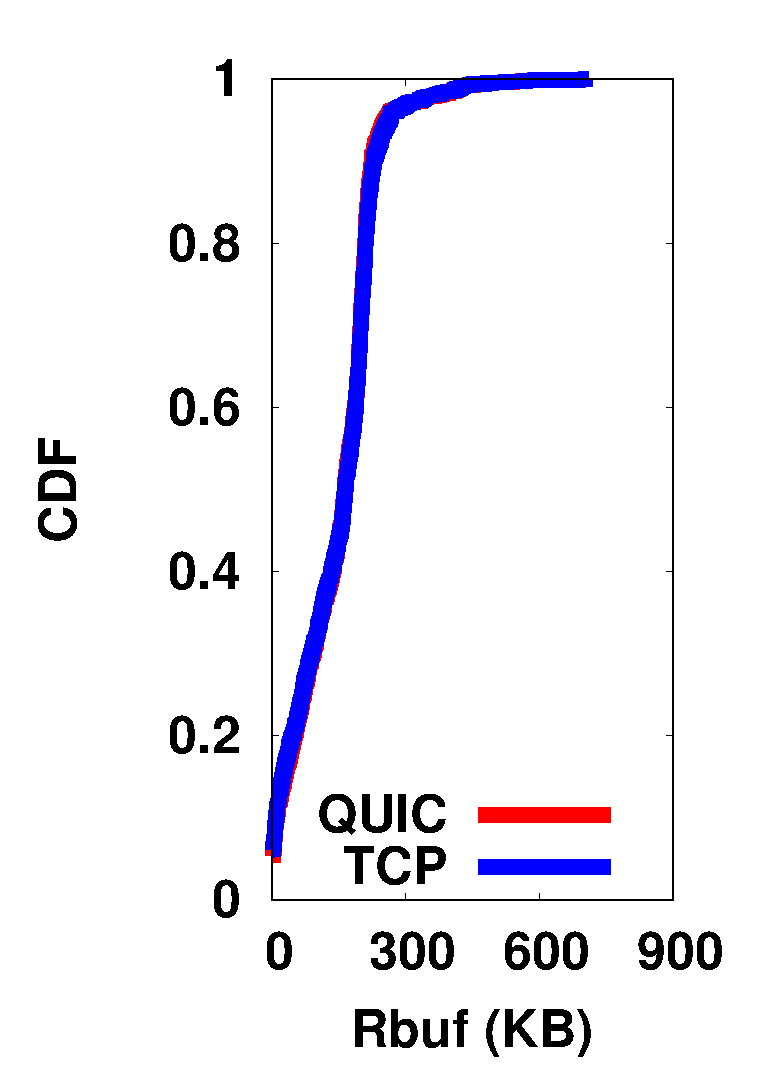
\includegraphics[width=0.32\linewidth]{img/CDF/plot_rbuf_bucket3}
%		}
        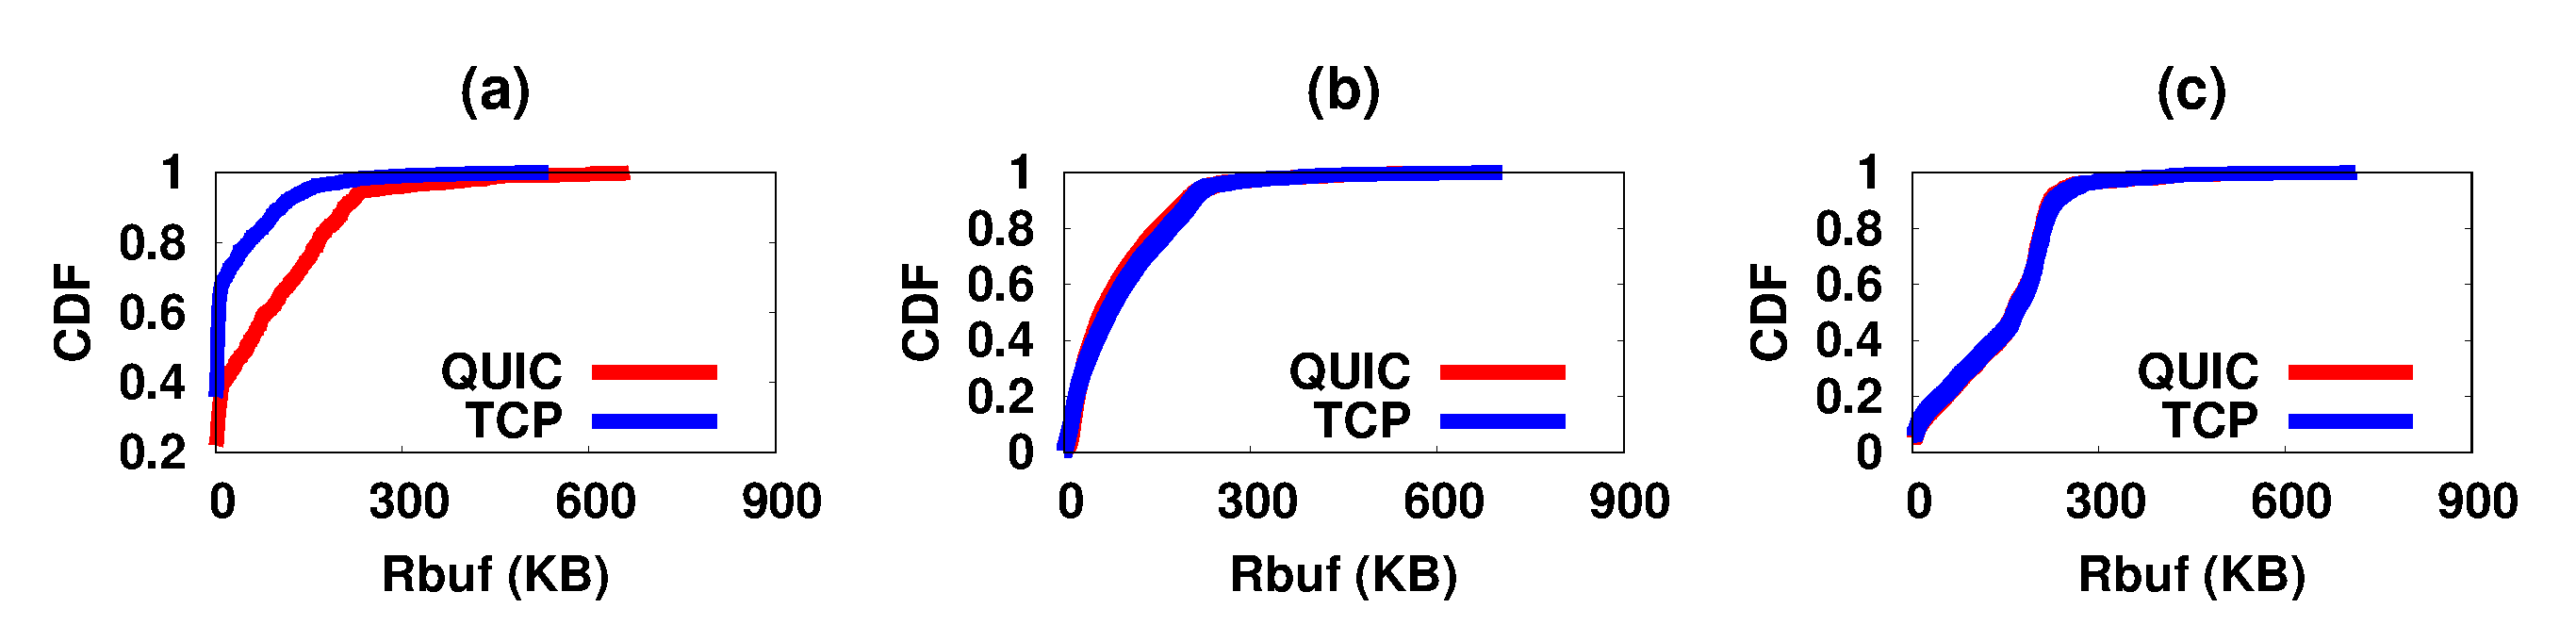
\includegraphics[width=\linewidth]{img/plotdata/CDF/Rbuf/plot_rbuf_bucket123}
		\caption{\label{fig:rbuf}Client buffer occupancy with respect to various bandwidth levels: (a) $\leq 64$ Kbps, (b)  between $64$ and $1024$ Kbps, (c) $> 1024$ Kbps}
	\end{center}
\end{figure}


\fig\ref{fig:rbuf} shows playback buffer occupancy distribution at the YouTube client in terms of \ac{CDF} for various \textit{rbuf} values extracted from the playback requests. We observe that at high bandwidth, there is not much difference between \ac{TCP} and \ac{QUIC} in terms of playback buffer occupancy. However, at low bandwidth, \ac{QUIC} fills up the playback buffer faster than \ac{TCP}, resulting in higher values of \textit{rbuf}. 
%has higher tendency towards higher \textit{rbuf} values when compared to TCP, indicating that QUIC tries to fill the client buffer fast even when the bandwidth is low. 
YouTube uses playback buffer occupancy as a feedback for video quality adaptation~\cite{mondal2017youtube,krishnappa2013dashing}
% -- if the buffer fills fast, the adaptive streaming client assumes the channel quality to be good, and switches to a high quality level for next video segment requests. However, as we have observed earlier, 
This sometime triggers a unsuccessful quality upgrade request for \ac{QUIC} enabled streaming, as the actual channel quality may not be suitable for high bitrate video streaming. This results in large number of rebuffering (\fig\ref{fig:bitrate_rebuffering}(b)) and comparatively high data waste (\fig\ref{fig:data_wasted}).

%This majorly implies that the chance for buffering is lower for QUIC when compared to TCP as buffering mainly occurs at poor Internet speeds supporting the statement made by Google that there were fewer rebuffers when QUIC is used instead of TCP.


%\notesc{Merge the three plots in a single plot -- (a) Bandwidth $ \leq 64 $ Kbps, (b) $64$ Kbps $<$ Bandwidth $ \leq 1024$ Kbps, (c) Bandwidth  $> 1024$ Kbps} \noteam{Done. \fig\ref{fig:rbuf}}
\begin{comment}
\begin{figure}[!ht]
    \centering
    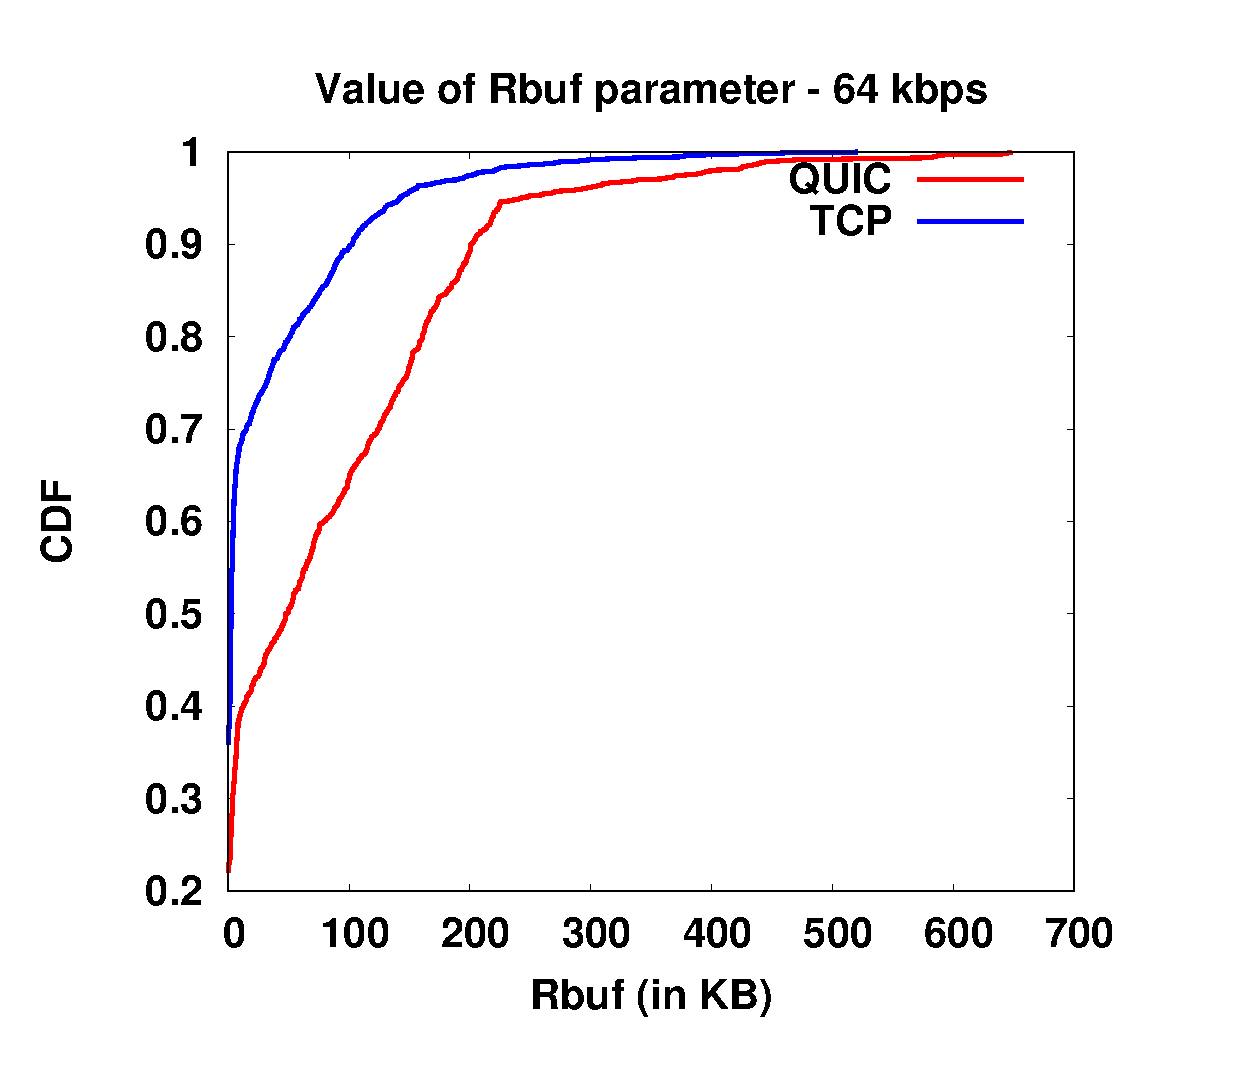
\includegraphics[width=0.9\linewidth]{img/CDF/plot_rbuf_65536}
    \caption{CDF of rbuf at 64 kbps}
    \label{fig:rbuf6556}
\end{figure}

\begin{figure}[!ht]
    \centering
    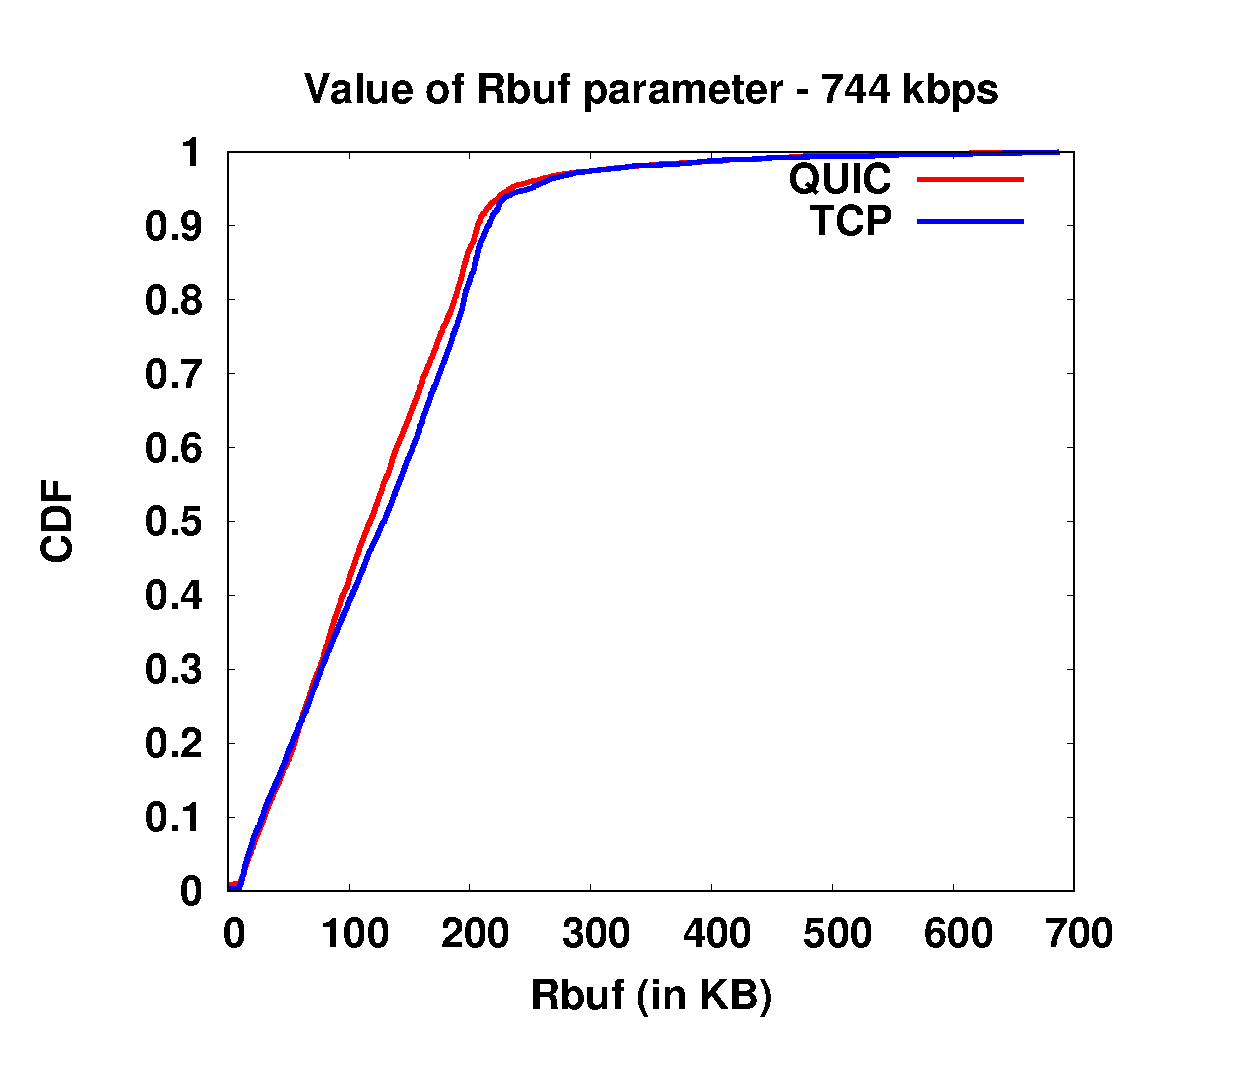
\includegraphics[width=0.9\linewidth]{img/CDF/plot_rbuf_761856}
    \caption{CDF of rbuf at 744 kbps}
    \label{fig:rbuf761856}
\end{figure}
\begin{figure}[!ht]
    \centering
    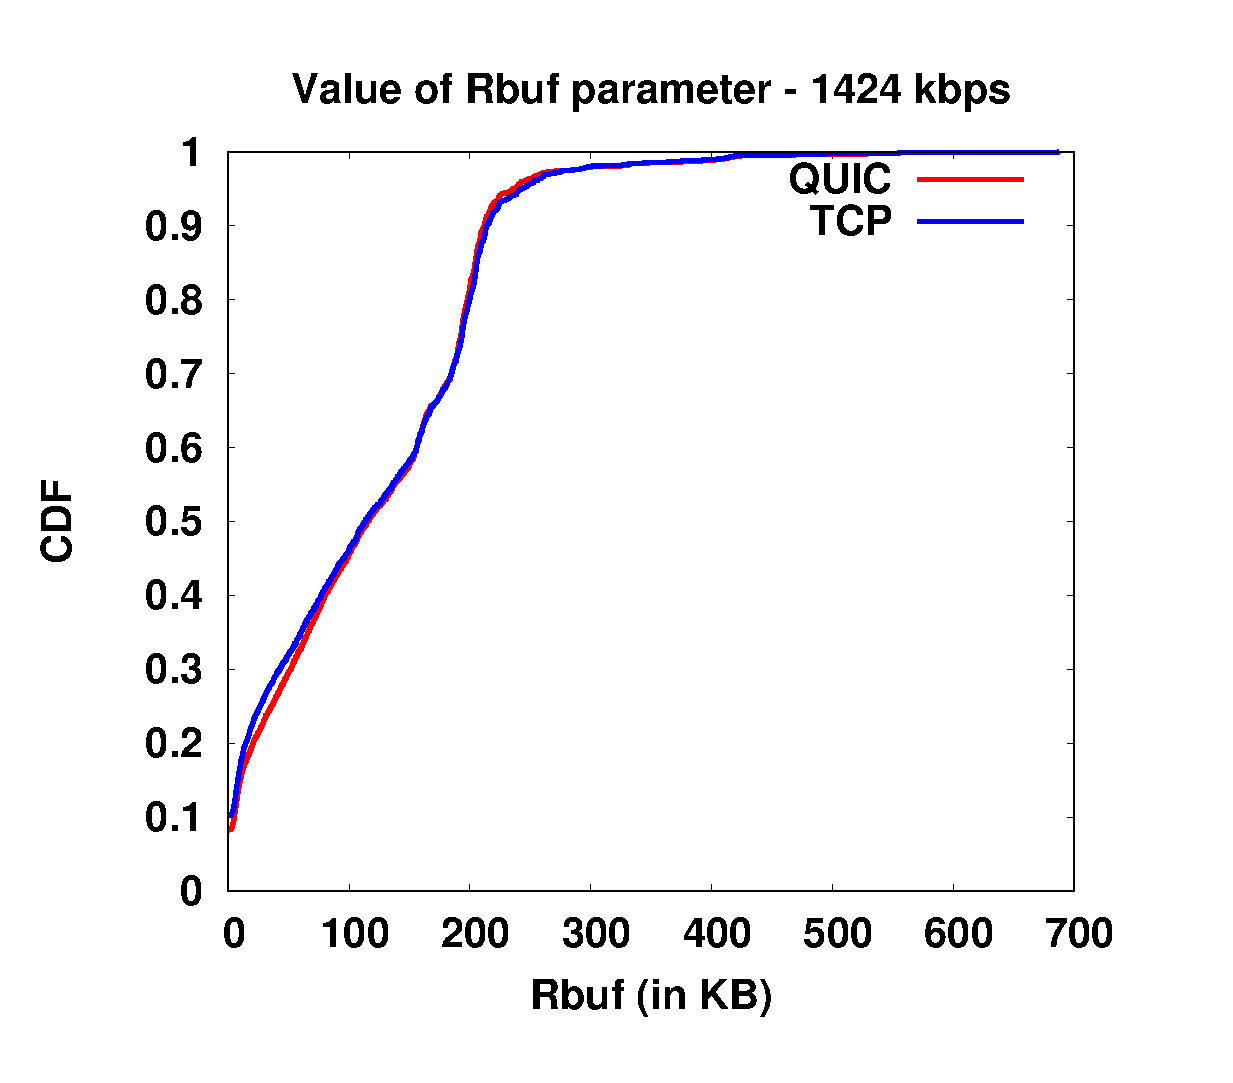
\includegraphics[width=0.9\linewidth]{img/CDF/plot_rbuf_1458176}
    \caption{CDF of rbuf at 1424 kbps}
    \label{fig:rbuf761}
\end{figure}
\end{comment}

%\subsubsection{Segment Length with respect to Various Bandwidth levels}
%As described earlier \textit{range} parameter consists of two values separated by a \\dash (-) and they define the byte range of the video for a itag value that the client requests from the server. We have taken the difference between these two values and plotted the CDF plots. At higher bandwidth levels the two protocols doesn't differ but at lower bandwidth QUIC has a greater tendency to request data in larger chunks when compared to TCP. Since QUIC is requesting in larger chunks we can estimate that it requires lesser number of requests to server to fetch data which is confirmed by the Fig. 3.8-3.10.




\begin{comment}
\begin{figure}[!ht]
    \centering
    \includegraphics[width=0.9\linewidth]{img/CDF/plot_range_65536}
    \caption{CDF of range at 64 kbps}
    \label{fig:range6556}
\end{figure}
\begin{figure}[!ht]
    \centering
    \includegraphics[width=0.9\linewidth]{img/CDF/plot_range_761856}
    \caption{CDF of range at 744 kbps}
    \label{fig:rang4761}
\end{figure}
\begin{figure}[!ht]
    \centering
    \includegraphics[width=0.9\linewidth]{img/CDF/plot_range_1458176}
    \caption{CDF of range at 1424 kbps}
    \label{fig:rang761}
\end{figure}
\end{comment}
\subsubsection{Segment Length Adaptation}

\begin{figure}[!t]
	\captionsetup[subfigure]{}
	\begin{center}
%		\subfloat[\label{fig:segment_bucket1}Bandwidth $ \leq 64 $ Kbps]{
%			\includegraphics[width=0.32\linewidth]{img/CDF/plot_segment_bucket1}
%		}
%		\subfloat[\label{fig:segment_bucket2} $64$ Kbps $<$ Bandwidth $ \leq 1024$ Kbps]{
%			\includegraphics[width=0.32\linewidth]{img/CDF/plot_segment_bucket2}
%		}
%		\subfloat[\label{fig:segment_bucket3}Bandwidth  $> 1024$ Kbps]{
%			\includegraphics[width=0.32\linewidth]{img/CDF/plot_segment_bucket3}
%		}
        \includegraphics[width=\linewidth]{img/plotdata/CDF/Segment/plot_segment_bucket123}
		\caption{\label{fig:segment}Segment length with respect to various bandwidth levels: (a) $\leq 64$ Kbps, (b)  between $64$ and $1024$ Kbps, (c) $> 1024$ Kbps}
	\end{center}
\end{figure}


Apart from video quality, YouTube also adapts the segment length~\cite{mondal2017youtube} -- to download data in larger chunks when the channel condition is good. We compare the segment length adaptation behavior for \ac{QUIC} and \ac{TCP} enabled streaming in \fig\ref{fig:segment}, which shows the \ac{CDF} of segment lengths for \ac{QUIC} and \ac{TCP} enabled streaming protocols. 
%Here we observe a behavior similar to the client buffer occupancy distribution. 
Under poor channel conditions, the YouTube client tries to download data in larger chunks for \ac{QUIC} enabled streaming. This is another factor behind the increased rebuffering and comparatively high data waste with \ac{QUIC}. The fast data download capability of \ac{QUIC} does not get converted to a proper video quality adaptation feedback for the YouTube streaming mechanism, where both the quality level and the segment size of the video chunks gets adapted dynamically. 

 
%This is another way of representing the \textit{range} parameter. From the number of bytes requested through range parameter we can convert it into duration of playback seconds using the bit-rates for the \textit{itags}. The trends will be similar to the CDF plots of \textit{range} with QUIC trying to request segments with longer duration when compared to TCP at lower bandwidths but at higher bandwidths the difference is not much.

%\notesc{Merge the three plots in a single plot. (a) Bandwidth $ \leq 64 $ Kbps, (b) $64$ Kbps $<$ Bandwidth $ \leq 1024$ Kbps, (c) Bandwidth  $> 1024$ Kbps}\noteam{Done. \fig\ref{fig:segment}}

\begin{comment}
\begin{figure}[!ht]
    \centering
    \includegraphics[width=0.9\linewidth]{img/CDF/plot_segment_65536}
    \caption{CDF of Segment Length at 64 kbps}
    \label{fig:seg6556}
\end{figure}
\begin{figure}[!ht]
    \centering
    \includegraphics[width=0.9\linewidth]{img/CDF/plot_segment_761856}
    \caption{CDF of Segment Length at 744 kbps}
    \label{fig:seg7621}
\end{figure}
\begin{figure}[!ht]
    \centering
    \includegraphics[width=0.9\linewidth]{img/CDF/plot_segment_1458176}
    \caption{CDF of Segment Length at 1424 kbps}
    \label{fig:seg761}
\end{figure}
\end{comment}


\begin{comment}
%\begin{addmargin}[2.1cm]{2.1cm}
\subsubsection{CDF for \textit{itag} with respect to various \textit{rbuf} ranges(buckets) }
The two protocols does not differ much with respect to \textit{rbuf}. When the buffer is smaller in amount they fetch all the itags but when the buffer is sufficiently large both the protocols fetch data only for higher itags as it is evident in the last two plots. QUIC makes more number of requests than TCP when the client has buffered large amount of data. This can be interpreted as QUIC's estimation that since buffer has large amount of data the rate of data consumption is less when compared to data fetched so bandwidth is sufficiently good and it can make further requests. It is also evident that most of the requests to server were made when the buffer is low in data as both the protocols interpret this as data depletion at a faster rate so they try to fetch data at a faster rate which means more number of requests made.

%\end{addmargin}

\begin{figure}[!ht]
    \centering
    \includegraphics[width=0.9\linewidth]{img/CDF/plot_itag_142367}
    \caption{Number of requests and CDF of itag for rbuf $<$139 KB}
    \label{fig:itag761121}
\end{figure}

\begin{figure}[!ht]
    \centering
    \includegraphics[width=0.9\linewidth]{img/CDF/plot_itag_284734}
    \caption{Number of requests and CDF of itag for rbuf 139-278 KB}
    \label{fig:itag65526}
\end{figure}
\begin{figure}[!ht]
    \centering
    \includegraphics[width=0.9\linewidth]{img/CDF/plot_itag_427101}
    \caption{Number of requests and CDF of itag for rbuf 278-417 KB}
    \label{fig:itag7612}
\end{figure}

\begin{figure}[!ht]
    \centering
    \includegraphics[width=0.9\linewidth]{img/CDF/plot_itag_569468}
    \caption{Number of requests and CDF of itag for rbuf 417-556 KB}
    \label{fig:itag65561}
\end{figure}
\begin{figure}[!ht]
    \centering
    \includegraphics[width=0.9\linewidth]{img/CDF/plot_itag_711837}
    \caption{Number of requests and CDF of itag for rbuf 556-695 KB}
    \label{fig:itag7611}
\end{figure}

\subsubsection{CDF for \textit{range} with respect to various \textit{rbuf} ranges(buckets) }
The behaviour of both the protocols is similar when the buffer is quite low or quite high but when the buffer is in the medium range QUIC and TCP show a different pattern. When the buffer is low both the protocols take a conservative approach and request the data in smaller chunks but QUIC requests the data in a slightly larger chunks. When the buffer is above a threshold value QUIC and TCP differ in that QUIC tries to download the data in larger chunks when compared to TCP. When the buffer is sufficiently high both the protocols doesn't differ much.
\begin{figure}[!ht]
    \centering
    \includegraphics[width=0.9\linewidth]{img/CDF/plot_range_142367}
    \caption{CDF of range for rbuf $<$ 139KB}
    \label{fig:rabuf6556}
\end{figure}

\begin{figure}[!ht]
    \centering
    \includegraphics[width=0.9\linewidth]{img/CDF/plot_range_284734}
    \caption{CDF of range for rbuf 139-278KB}
    \label{fig:rabuf761856}
\end{figure}
\begin{figure}[!ht]
    \centering
    \includegraphics[width=0.9\linewidth]{img/CDF/plot_range_569468}
    \caption{CDF of range for rbuf 417-556KB}
    \label{fig:rabuf761}
\end{figure}
%\clearpage
\end{comment}




\subsection{Summary}
In this section, we developed a systematic analysis of web based adaptive streaming performance over \ac{QUIC} and compared it with \ac{TCP} enabled video streaming. We developed a testbed to automatically download $175$ YouTube videos with different quality levels and of different sizes using both \ac{QUIC} enabled and \ac{TCP} enabled streaming. From thorough analysis, we observed that although \ac{QUIC} improves data download performance even at poor network condition, the benefits do not get directly translated to adaptive video streaming over the web, when \ac{QoE} metrics are considered. 

This section primarily analyzed the performance from the context of YouTube \ac{ABR} streaming. In the next section, we discuss about a more generalized analysis, where we consider various recent \ac{ABR} streaming algorithms. 

\renewcommand{\relpath}[1]{Chapters/033.QUIC/}
\graphicspath{{Chapters/033.QUIC/}}
%\clearemptydoublepage

\begin{appendix}
\chapter[Extended results of Chapter]
\noindent


\end{appendix}

\renewcommand{\bibname}{References}
\bibliographystyle{abbrv}
%\bibliography{survey}


\addcontentsline{toc}{chapter}{Dissemination}
\chapter*{Dissemination}
\vspace*{0.5cm}
% \noindent
\renewcommand{\chaptermark}[1]{\markboth{}{\sffamily #1}}
\chaptermark{Dissemination}
\begin{center}
\textbf{\underline{Journals}}
\end{center}
\begin{enumerate}
\item journal 1
\end{enumerate}

\begin{center}
{\textbf{\underline{Conferences}}}
\end{center}
% \subsection*{Conferences}

\begin{enumerate}
\item conf 1

\end{enumerate}
% \endgroup
\noindent
% \rule{0.49\textwidth}{0.75pt} $_{\Diamond}$ \rule{0.49\textwidth}{0.75pt}\\

% \end{onehalfspacing}





\clearemptydoublepage

\end{document}
